% \newcommand{\region}[1]{\texttt{#1}}
\newcommand{\region}[1]{#1}


The Pore Pressure experiment (\cite{tz_monitoring}) was conducted during the excavation of the experimental chambers \region{ZK5-1J} and \region{ZK5-1S}. The experiment consisted of the following phases: 

\begin{enumerate} 
\item {\it Dec., 2023.} 
The system of 8 boreholes and 24 measurement cells, with 3 cells in each borehole, was designed via sensitivity-based design optimization under technical constraints, using a predictive 3D model (\cite{tz_design}).
The boreholes were designed with a minimum distance of 1~m from the planned excavations. 
\item {\it Jan., 2024.} The boreholes were drilled from the \region{L5} tunnel. 
\item {\it Feb., 2024.} Each borehole was inspected using video inspection, inclinometry, and OBI/ABI methods. 
A preliminary water-pressure test was conducted to identify exceptionally high permeability zones and to ensure sufficiently slow pressure changes in the measurement cells. 
\item The boreholes were instrumented with multipacker systems consisting of three pressure sensors installed in three hydraulically sealed cells using 2~MPa packers. 
\item Each measurement cell was pressurized to an initial pressure exceeding the expected pore pressure in the rock mass, and equilibration with the in-situ pore pressure was recorded by continuous pressure monitoring. 
\item {\it Mar., 2024.} Drill-and-blast excavation of the \region{ZK5-1S} and \region{ZK5-1J} chambers was performed in a total of 12 blasts of approximately 2~m each. 
\item {\it Sep., 2024.} A simple water-pressure test was conducted in each measurement cell. 
\item {\it Apr., 2025.} A water-pressure test with measurement of water flux was conducted in each measurement cell. 
\end{enumerate}

\begin{figure} 
\centering 
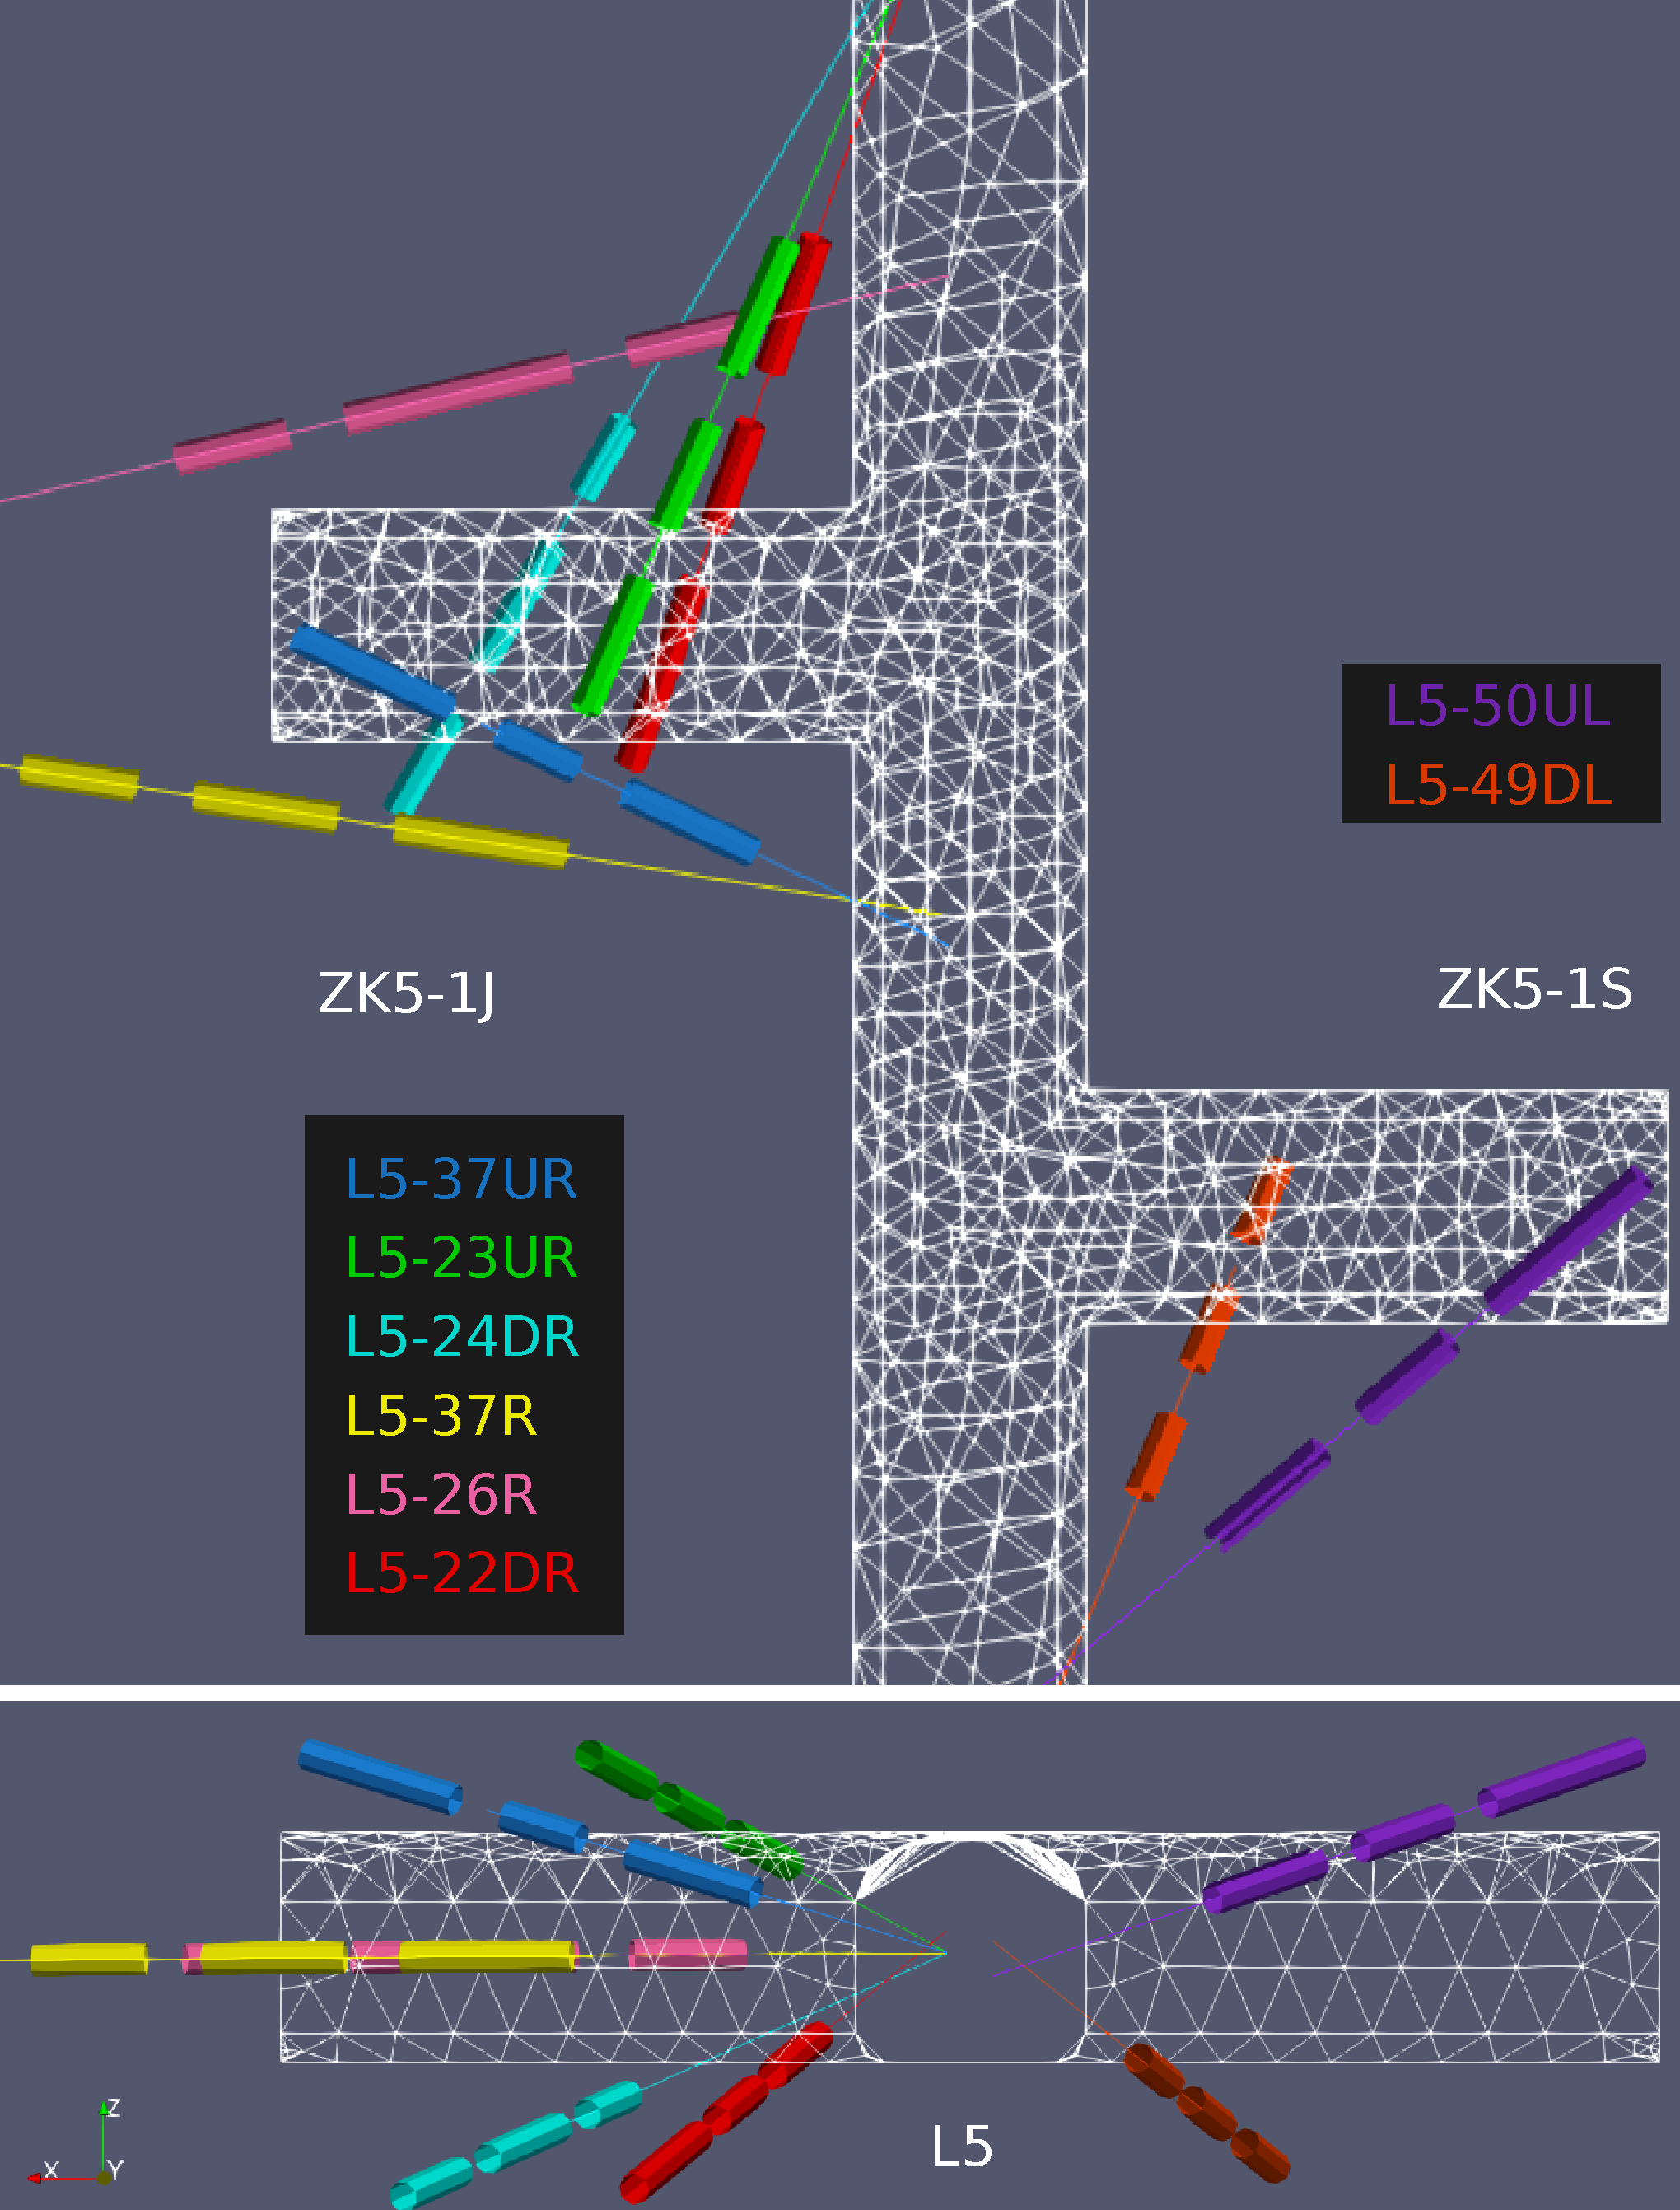
\includegraphics[width=0.65\linewidth]{PP_figs/boreholes_yz.pdf} 
\caption{Top and side views of the \region{ZK5-1S} and \region{ZK5-1J} chambers with borehole placement and measurement cells.} \label{fig:boreholes_yz} 
\end{figure} 

\begin{figure} 
\begin{center} 
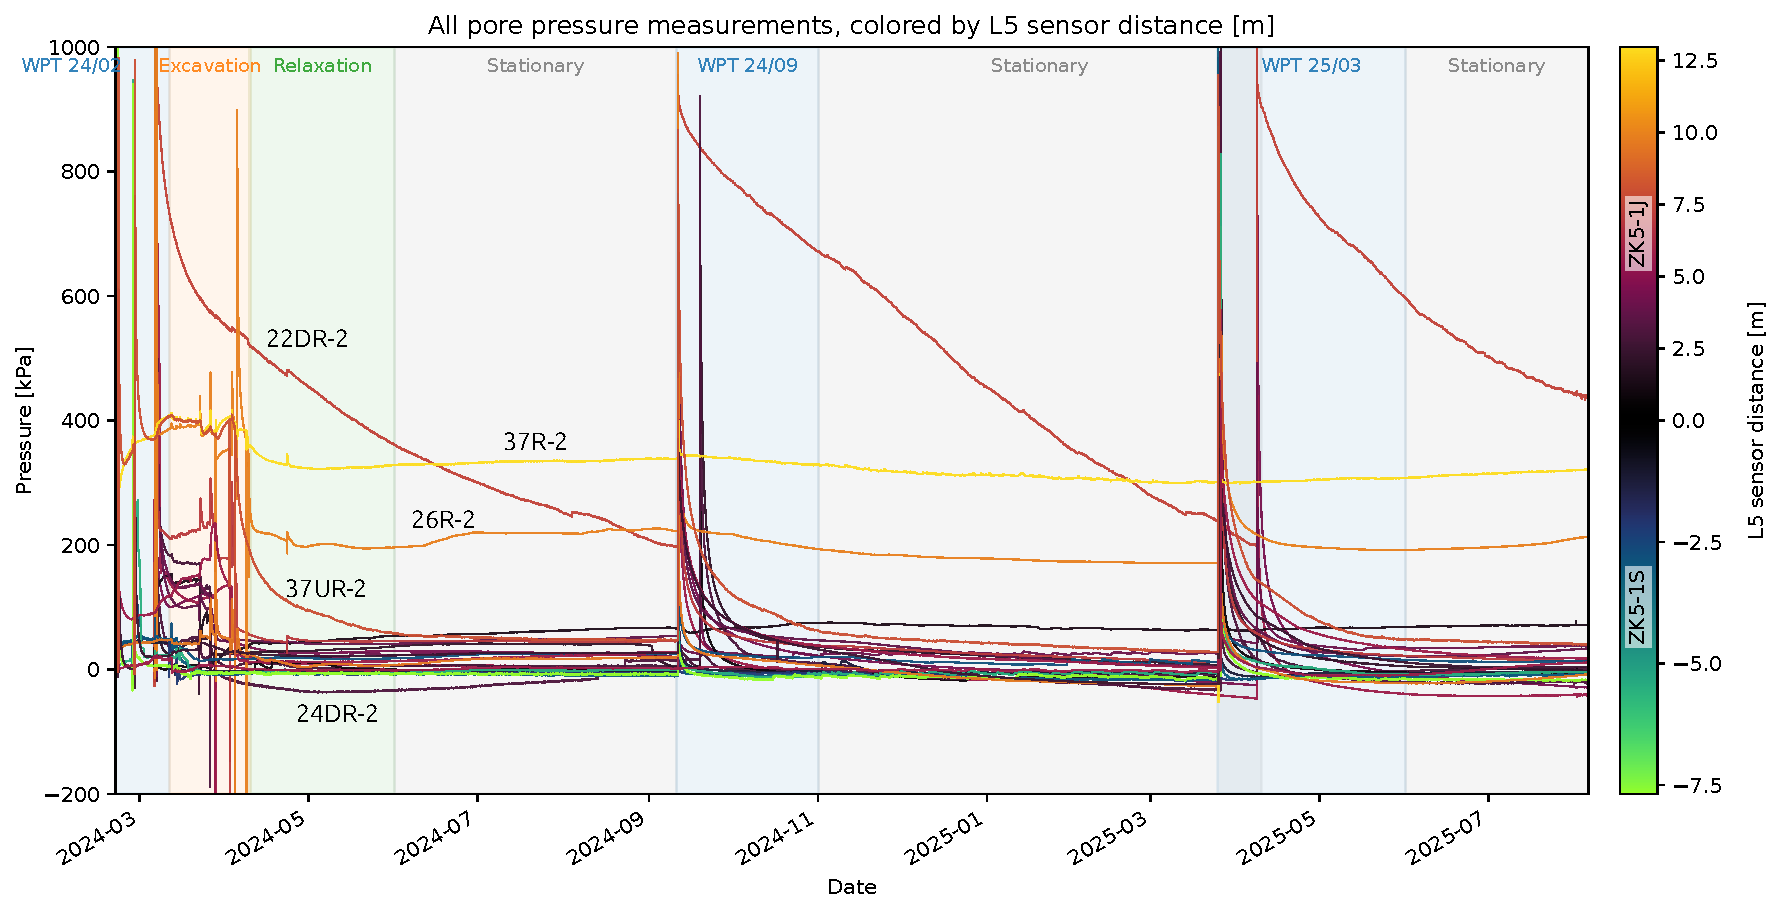
\includegraphics[width=\textwidth]{PP_figs/overview_plot_labels.pdf} 
\end{center} 
\caption{Overview of all pore-pressure measurements, colored by the distance of the sensor from the \region{L5} tunnel.} 
\label{fig:pp_overview} 
\end{figure}

The locations of the boreholes and measurement cells with respect to the \region{L5} tunnel and the excavated chambers are shown in Fig.~\ref{fig:boreholes_yz}. Only two boreholes are placed around the northern chamber \region{ZK5-1S}, where lower rock quality was expected. Six boreholes are located around the southern chamber \region{ZK5-1J}: two upward (\region{UR}), two downward (\region{DR}), and two horizontal (\region{R}) on the chamber sides. The placement was strongly constrained by technical limitations. Three pressure-measurement cells per borehole, depicted as colored cylinders, were delimited by rubber packers.

Throughout this chapter, pressure sensors are denoted by the borehole name (with the leading '\region{L5-}' omitted) followed by the position index. For example, \region{22DR-0} denotes the sensor closest to the \region{L5} tunnel in borehole \region{L5-22DR}.

An overview of all collected measurements up to August~2025, together with the essential experimental phases, is shown in Fig.~\ref{fig:pp_overview}. Each line corresponds to a single installed sensor and is colored by the distance of the sensor from the \region{L5} tunnel. The positive direction is toward the south for sensors around \region{ZK5-1J}. Measurements from several distinct pressure sensors are labeled. As expected, these correspond to sensors located in the outermost cells, at least 5~m from the \region{L5} tunnel.

The initial \Gls{WPT}s were completed only one week before the first excavation, leaving insufficient time for the measured pressures to return to equilibrium with the background pore pressure. This effect is most evident for sensor \region{22DR-2}, which was unable to relax to equilibrium even after six months. Other sensors that were slightly affected include \region{37R-0}, \region{26R-0}, \region{22DR-0}, \region{23UR-0}, and \region{24DR-2}.

\subsection{Overview of excavation}

We divided the 24 pressure sensors into two groups based on the amplitude of their pressure changes. 
The pore-pressure response to excavation for the twelve most responsive sensors is shown in Fig.~\ref{fig:large_p}, 
while the sensors with smaller responses are shown in Fig.~\ref{fig:small_p}.

All sensors exhibiting large responses are located in the southern boreholes; therefore, their response to the first 
six blasts in the northern chamber is minimal. A significant response is observed during the last six blasts, 
corresponding to the progressive advance of the southern chamber excavation face to distances of 1.6~m, 3.5~m, 5.5~m, 7.2~m, 9.3~m, and 10~m.


\begin{figure}[h]
    \begin{center}
    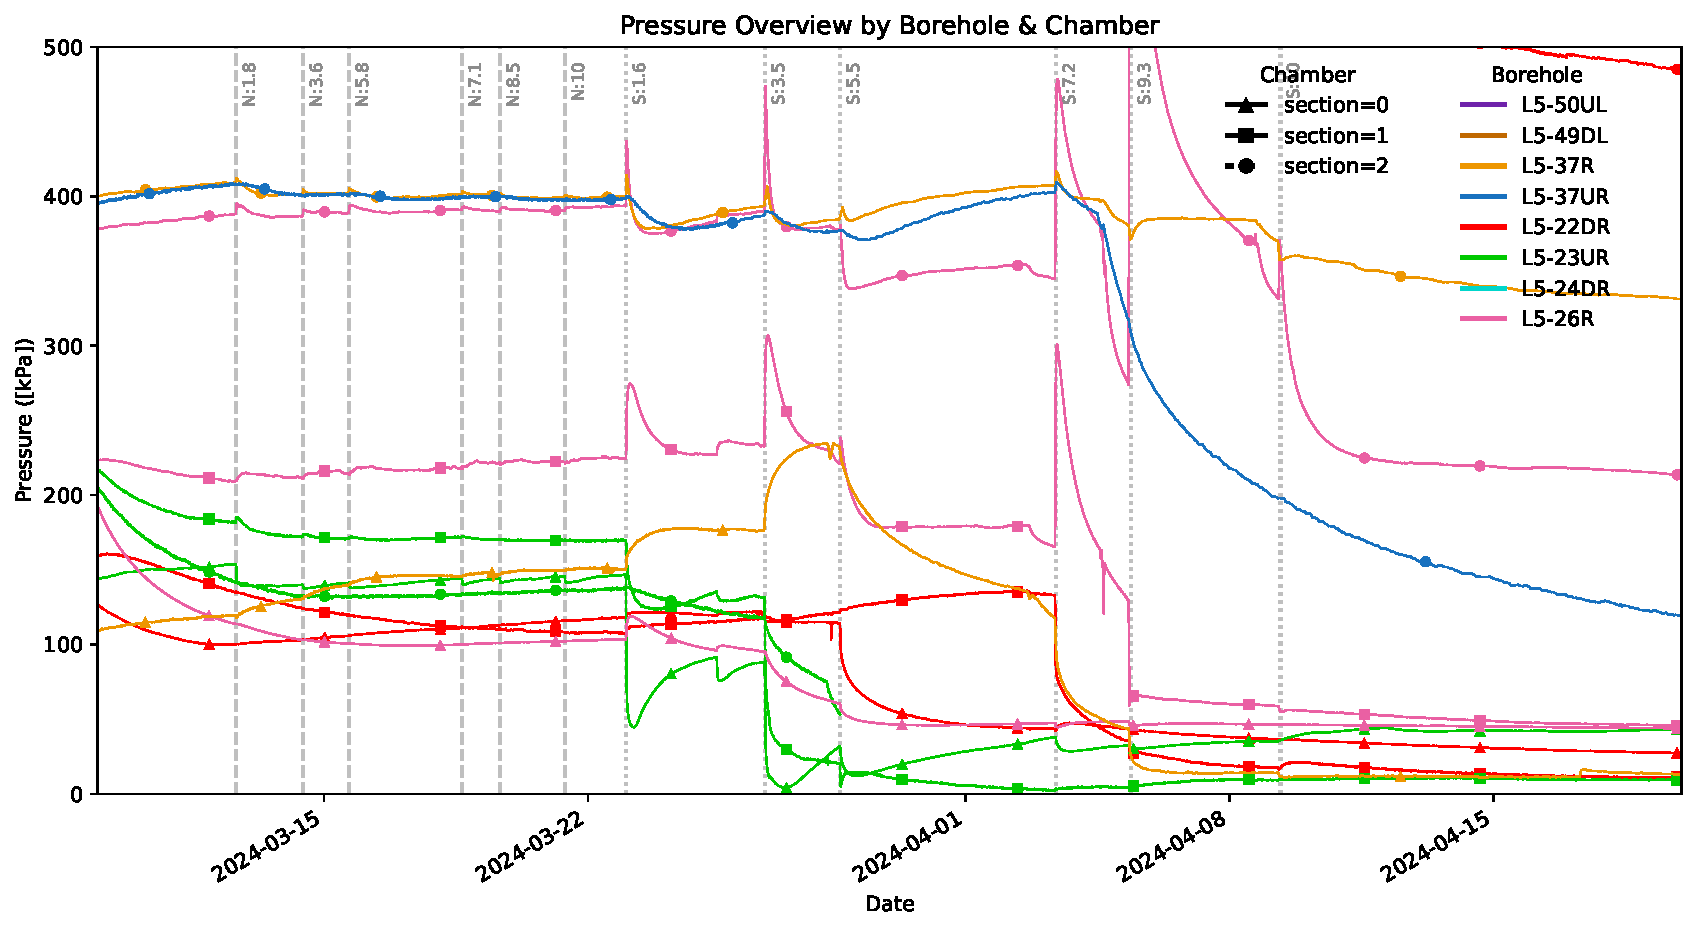
\includegraphics[width=\textwidth]{PP_figs/excavation_large_p.pdf}
    \end{center}
    \caption{Pore-pressure monitoring during excavation for sensors exhibiting the largest pressure response. 
    Blast times are indicated by vertical lines.}
    \label{fig:large_p}
\end{figure}

The pressure record of sensor \region{22DR-2} lies outside the plotted range. Its response to excavation is negligible and, unfortunately, cannot be recovered by simple subtraction of the long-term trend. This measurement cell effectively behaves as a closed cavity pressurized to approximately 600~kPa. 
Changes in external pressure do not directly affect the internal pressure unless the external pressure exceeds the internal pressure; they only influence the deformation of the cell. However, the excavation-induced pressure changes remain below 500~kPa, with the exception of a short pressure peak observed in sensor \region{26R-2}.



The majority of jumps in the pressure values, or in their time derivatives, are associated with blasting and the resulting immediate changes in the stress field. However, less pronounced changes, synchronized across all sensors, appear prior to each blast. As most of these events correspond to drops in the pressure derivative, they may be attributed to drilling of the blast boreholes and the associated drainage of hydraulically active fractures. An exception is the event occurring shortly after 2024/03/25, which consists of a downward jump in \region{23UR-0} and \region{23UR-2}, but also, surprisingly, of upward jumps in \region{26R-1} and \region{26R-0}. These upward jumps cannot be explained by plain Darcy flow in a heterogeneous medium. A plausible explanation is that drainage of a nearby fracture releases compressive stress acting on a subparallel fracture, causing it to open and hydraulically connect the affected measurement cells to a region of higher pore pressure.

A hydro-mechanical model assuming homogeneous rock-mass properties predicts positive pressure peaks 
in locations above and below the excavated chamber, and pressure drops on the lateral sides. 
The observed response, however, is markedly different, most likely due to the fracture network, 
with a possible contribution from foliation-induced anisotropy. 
The most significant positive pressure peaks are observed in cells~1 and~2 of the lateral borehole 
\region{26R}, whereas typical pressure drops appear in cells~0 and~1 of the upward borehole \region{23UR}. 
Curved signal tips, particularly visible in \region{23UR}, indicate that the dominant source of these 
pressure changes is hydraulically located farther away from the directly measured water volume.

All blasting events are accompanied by significant pressure jumps, with a single exception. 
During the third blast, with the excavation face located 5.5~m from \region{L5}, a sudden pressure drop 
is observed in \region{26R} and less pronounced drops occur in other sensors. 
This suggests that the rock mass affected by this blast is hydraulically connected to a highly 
conductive fracture. This interpretation is consistent with subsequent geological mapping, 
which indicates the presence of a conductive zone at this location. 
The third blast has also damaged the sensor \region{23UR-2} indicating direct hydraulic connection to the 
excavation through a major fracture.


The pressure readings from sensor \region{37R-0}, located approximately 5~m from \region{L5}, are anomalous. 
The pressure increases monotonically up to the third blasting event, even during excavation of the 
northern chamber. This behavior suggests a hydraulic connection to a large fracture that lost pressure 
during drilling of the measurement boreholes, followed by a slow recovery toward the initial state. 
This recovery is ultimately interrupted by the third blast, during which the fracture becomes 
connected to atmospheric pressure, causing the measured pressure to decay toward zero.

\begin{figure}[h]
    \begin{center}
    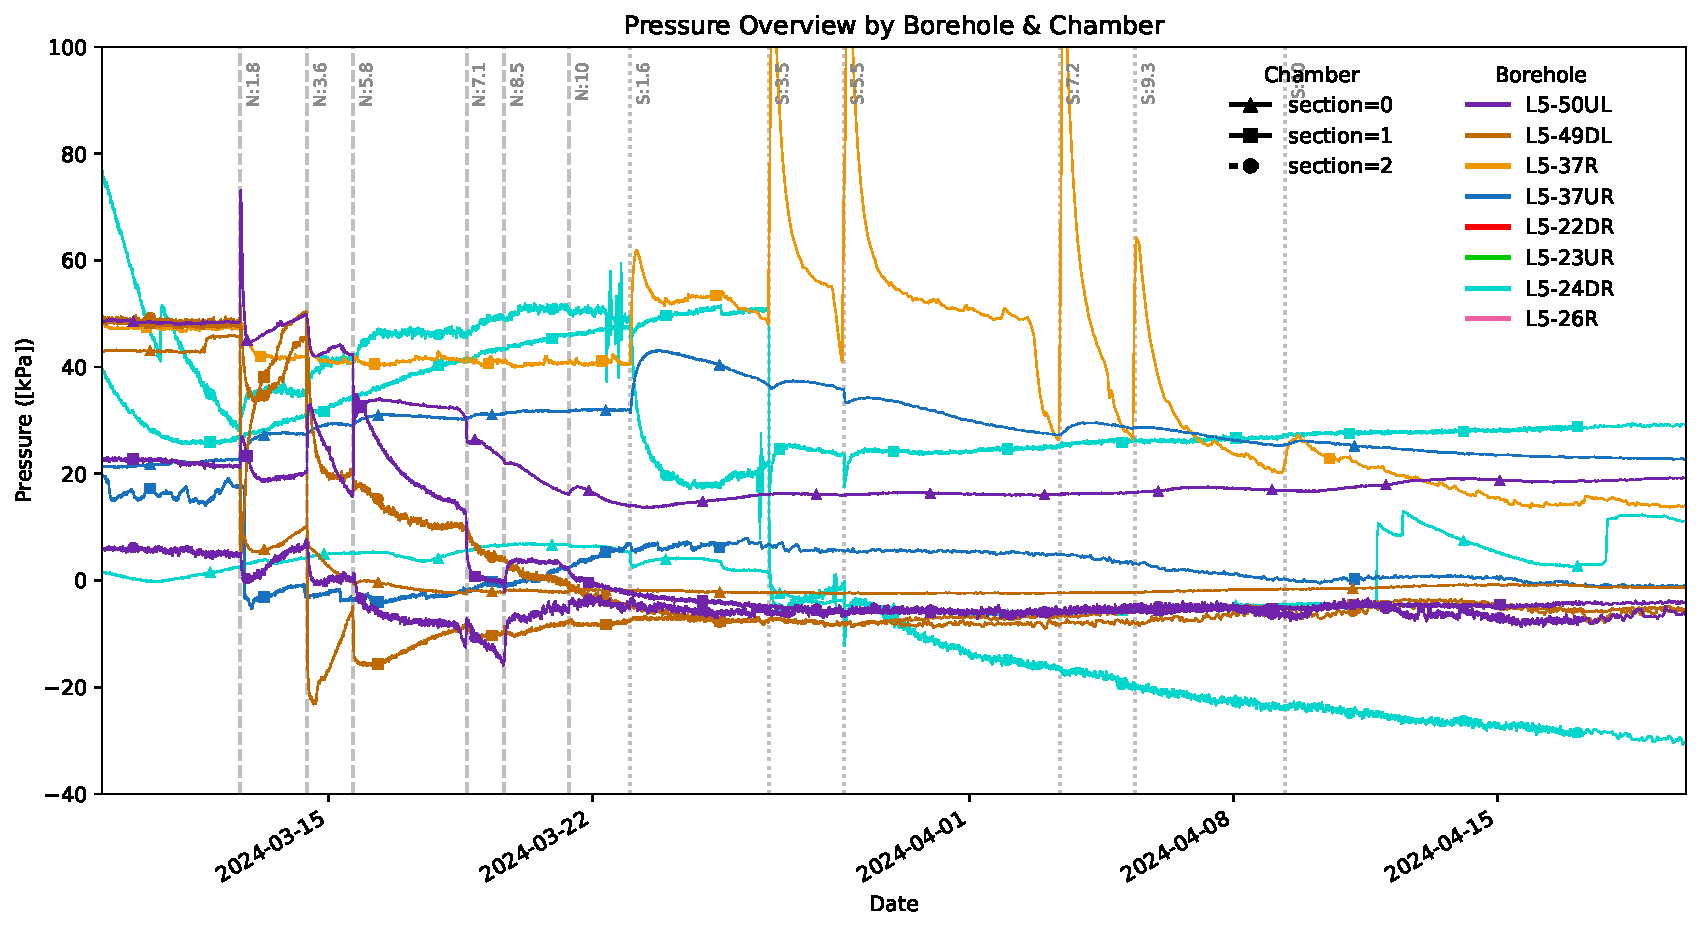
\includegraphics[width=\textwidth]{PP_figs/excavation_small_p.pdf}
    \end{center}
    \caption{Pore pressure monitoring during excavation - small pressure cells.}
    \label{fig:small_p}
\end{figure}

The small pressure readings are summarized in Fig.~\ref{fig:small_p}.
The signal from sensor \region{37R-1} exhibits characteristic peaks, 
but they are approximately one order of magnitude smaller 
than those observed in sensors~0 and~2 within the same borehole. 
This suggests a fracture connection to a zone with low initial pressure, 
possibly to the \region{L6} tunnel. 
Although this measurement cell is located relatively close to the 
excavated chamber, there appears to be no highly conductive connection 
to the new excavation: all blast-induced peaks are present, and the 
subsequent pressure decay is slow, approaching a value slightly above zero.

Sensor \region{37UR-0} exhibits behavior similar to that of \region{37R-0}. 
The remaining southern readings are for the sensors located in borehole \region{24DR}, 
which follows the expected conductive zone. 
A surprising \textquote{reconnection} effect is observed during the second 
southern blast, when the pressure in \region{24DR-1} drops to the level of 
\region{24DR-2}, while the latter subsequently decreases further, falling 
below the pressure recorded in \region{24DR-0} and reaching values below 
zero (atmospheric pressure).

The northern sensors respond to the northern blasting events with 
patterns similar to those observed in the southern boreholes, but with 
much smaller amplitudes. This behavior is attributed to overall higher 
hydraulic conductivity and reduced rock stiffness in the northern part 
of the excavation.





\subsection{Water pressure test model}

Observed pressure relaxation following water pressure tests often does not
correspond to the response of a homogeneous material. We therefore employ a
simple heterogeneous hydraulic model to characterize rock heterogeneity in the
vicinity of the measured borehole cells.

\begin{figure}[h]
    \centering
    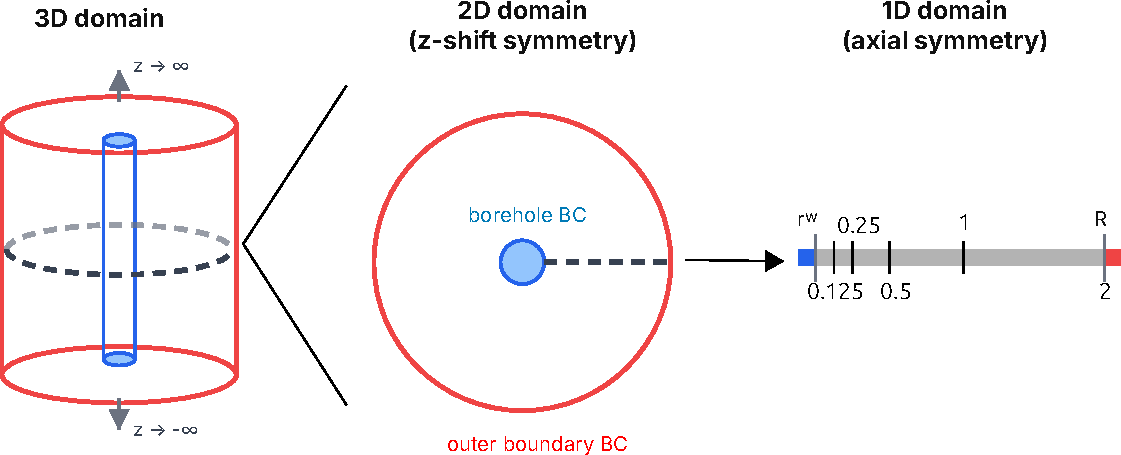
\includegraphics[width=0.8\linewidth]{PP_figs/conceptual_model_schema.pdf}
    \caption{Schematic illustration of the model simplifications.}
    \label{fig:model_simple}
\end{figure}

Starting from a three-dimensional Darcy flow model with storativity, we first
assume the measuring cell to be infinitely long with constant properties
along the borehole axis (see Fig.~\ref{fig:model_simple}). This allows the
problem to be reduced to two dimensions. Rewriting the resulting model in polar
coordinates and assuming axial symmetry, we further reduce it to a one-
dimensional radial Darcy flow model with a heterogeneous storativity (or specific storage) field
$S = S(r)$ $\bunit{1/m}$ and hydraulic conductivity field $k = k(r)$ $\bunit{m/s}$:
\[
S(r)\,\partial_t p(t,r)
= \frac{1}{r}\,\partial_r\!\left(
r\,k(r)\,\partial_r p(t,r)
\right)
\quad \text{in } (0,T)\times(r_w,R).
\]

Here, $p$ denotes the pressure head $\bunit{m}$, $r_w$ is the borehole radius $\bunit{m}$,
and $R$ is the outer radius of the computational domain $\bunit{m}$. 
To recover physically meaningful volumetric
fluxes, we consider a finite slab of thickness $L$ $\bunit{m}$ in the axial ($z$)
direction, representing the length of the measuring cell.

For a compact isotropic rock, the storativity is modeled as a combination of
water and rock compressibility,
\[
S(r) = \rho_w g\left(\phi c_f + (\alpha - \phi)c_s(r)\right),
\]
where $\rho_w$ $\bunit{kg\,m^{-3}}$ is the fluid density, $g$ $\bunit{m\,s^{-2}}$ is
gravitational acceleration, $\alpha$ $[-]$ is the Biot's coefficient , $\phi$ $[-]$ is porosity, $c_f$ $\bunit{Pa^{-1}}$ is the
compressibility of water, and $c_s$ $\bunit{Pa^{-1}}$ is the compressibility of the
dry rock skeleton. The latter is expressed in terms of the heterogeneous
Young’s modulus $E(r)$ $\bunit{Pa}$ and Poisson’s ratio $\nu$ $[-]$ as
\[
c_s(r) = \frac{3(1-2\nu)}{E(r)}.
\]
These relations primarily represent microscale storativity mechanisms and
serve to link the effective storativity, which is not directly measurable, to
elastic rock properties. Macroscopic poroelastic effects may also be captured
through this formulation, albeit with an effective (possibly nonphysical)
Young’s modulus.

\paragraph{Boundary conditions.}
\begin{itemize}
    \item At the borehole wall $r = r_w$, we assume a linear relationship
    between the volume change of the measuring cell and pressure head
    through a compliance factor:
    \[
        \frac{dV}{dt} = L\,\rho_w g\,c_b\,\partial_t p,
        \qquad
        c_b = \pi r_w^2 \left(
        c_f + \frac{2(1-\nu)(1-\nu^2)}{E(r_w)}
        \right),
    \]
    where $V$ $\bunit{m^3}$ is the cell volume and $c_b$ $\bunit{m^2\,Pa^{-1}}$ is the
    compliance per unit length.

    Conservation of volume requires that the rate of volume change equals the
    radial flux at the borehole wall,
    \[
        \rho_w g\,c_b\,\partial_t p(t,r_w)
        = q(t)
        := 2\pi r_w k(r_w)\,\partial_r p(t,r_w),
    \]
    where $q$ $\bunit{m^2\,s^{-1}}$ denotes the radial flux from the borehole cell
    into the surrounding domain, defined according to the sign convention
    adopted here. The corresponding volumetric flux is given by
    $Q(t) = L\,q(t)$ $\bunit{m^3\,s^{-1}}$.

    \item At the outer boundary $r = R$, the pressure head is prescribed as
    \[
        p(t,R) = p_R,
    \]
    where $p_R$ $\bunit{m}$ is the \emph{equilibrium pressure head}. 
  
\end{itemize}

The equilibrium pressure is the only Dirichlet condition in the model and therefore sets the
unique long-time limit of the solution: for $t \to \infty$, the pressure field
relaxes toward a spatially uniform state with $p(t,r) \to p_R$.

Physically, $p_R$ represents the ambient formation pressure head in the
vicinity of the measuring cell. In the absence of hydraulically connected
large-scale features, it can be interpreted as a local background level, i.e.,
a representative average over the neighborhood of the borehole cell. If,
however, the cell is connected to a far-reaching conductive fracture or
network, the relaxation may be controlled by that feature and the effective
equilibrium level may reflect a more distant hydraulic boundary.

The problem is discretized using linear (P1) finite elements with radially
distributed nodes following a geometric progression, as illustrated in
Fig.~\ref{fig:model_simple}. The initial condition is defined by setting the
pressure head in the domain to $p_R$, while the initial pressure head at the
borehole wall, $p(r_w)=p_w$, is set to the maximum pressure reached during the
water pressure test.

\subsection{Bayesian inversion for water pressure tests}

The WPT model was parameterized by the equilibrium pressure $p_R$
(\verb|p_far| in the plots) and by spatially varying hydraulic conductivity
and Young’s modulus. Both $k$ and $E$ were represented by values defined on
five finite elements, resulting in 11 inversion parameters in total.

A normal prior distribution was prescribed for the equilibrium pressure,
$p_R \sim \mathcal{N}(\mu = 60,\sigma = 25)$~$\bunit{kPa}$, for the majority of the
measured cells. These values were adapted where necessary to reflect the expected long-term  limit of the observed pressure at individual locations.

Lognormal prior distributions were assumed for the material parameters. In
logarithmic space, the priors were defined as
\[
\log_{10} E \sim \mathcal{N}\!\left(\mu = \log_{10}(5\times10^{9}),
\sigma = 1.2\right), \qquad
\log_{10} k \sim \mathcal{N}\!\left(\mu = \log_{10}(1\times10^{-9}),
\sigma = 2\right),
\]
with $E$ expressed in pascals $\bunit{Pa}$ and $k$ in meters per second $\bunit{m/s}$.
Spatial variability of each parameter was modeled using an exponential
correlation structure with correlation length $\lambda = 0.1 \munit{m}$. The
$p_R$, $k$, $E$ variables were treated as
statistically independent, resulting in a block-diagonal covariance
structure.

All remaining parameters were kept fixed during the inversion:
$r_w = 0.039 \munit{m}$, $R = 2 \munit{m}$, $\alpha = 0.2$, $\phi = 0.02$, $\nu = 0.25$, and
$c_w = 4.5\times10^{-10} \munit{Pa^{-1}}$.

The initial pressure was taken from the first measured pressure value. The
remaining pressure time series was used for model calibration assuming
independent Gaussian measurement errors with a standard deviation of
$3 \munit{kPa}$. 

The inversion was conducted for both the initial WPTs performed prior to
excavation and for the final WPTs carried out in autumn~2025. For the latter
tests, measurements of the water flux at the initial peak pressure were
available and incorporated in the inversion, assuming a relative standard
deviation of $2~\%$. Pressure and flux observations were combined additively in the
likelihood function. Inclusion of the flux information significantly reduced
the ambiguity between explaining the observed pressure evolution by
variations in hydraulic conductivity or by variations in rock stiffness.

Bayesian inference was carried out using a parallel implementation of the
DREAM algorithm (\cite{Vrugt_Markov_2016}), employing 20 Markov chains with
30\,000 samples per chain. The parallel DREAM sampler was implemented using
the \texttt{TinyDA} library.

\subsection{Interpretation of water pressure tests}
We performed the Bayesian inversion for each measurement cell in two stages. First,
only the pressure time series from the WPTs conducted before excavation were used.
Second, the pressure measurements were combined with the water-flux data obtained
during the WPTs in 2025. One of the main objectives was to estimate the equilibrium
pressure before and after excavation.


Figure~\ref{fig:pressure_summary} summarizes the posterior distributions of the
equilibrium pressure $p_R$ using boxplots for individual cells. Outliers were removed
using the standard 1.5~IQR rule. For comparison, the last pressure values recorded
before excavation (2024) and at the end of the available data in 2025 are also shown.
In some cases, the inversion yields very noisy predictions, mainly due to short data
intervals or non-monotonic pressure time series.

A comparison of water fluxes at the peak pressure for the 2024 and 2025 WPTs is shown
in Fig.~\ref{fig:flow_summary}. The predicted fluxes for both 2024 (blue, two independent runs) 
and 2025 (red) were computed solely from the pressure time series. For 2025, the directly
measured fluxes and their estimated uncertainties are shown in green. In many cells,
the predicted and measured fluxes differ significantly according to the Welch test;
these cells are highlighted in red. For such cases, the inversion based solely on the
initial WPTs provides little useful information.

Overall, the Bayesian inversion provides mainly qualitative insights. The simplistic 1D model cannot reproduce several behaviours observed during and after the initial WPTs (Fig.~\ref{fig:init_wpts}). These include non-monotonic pressure evolution in some 
 measurement cells (e.g., \region{L5-37R}), possibly reflecting a partially drained initial state; apparent interactions between neighbouring cells (e.g., \region{L5-37R} and \region{L5-37UR}); and anomalous responses in \region{L5-50UL} that may even be influenced by the WPT performed in \region{L5-37UR} on the opposite side of \region{L5}.

Despite these limitations, the inversion remains useful in specific cases. It can yield more precise estimates of the equilibrium pressure, and it clearly highlights the added value of direct water-flux measurements during WPTs. Although the model can reproduce strongly non-monotonic signals (e.g., sensor \region{37R-2}), it does so only by inferring highly heterogeneous hydro-mechanical parameters that fall outside a physically plausible range.


In the following sections, we describe notable features of the twelve cells showing
the most significant responses. We then provide a summary for the remaining six south
cells and the six north cells. For each sensor, we compare the WPT responses using
stitched plots and comment on the corresponding inversion results.

\begin{figure}[t]
  \centering
  \begin{subfigure}[t]{0.49\textwidth}
    \centering
    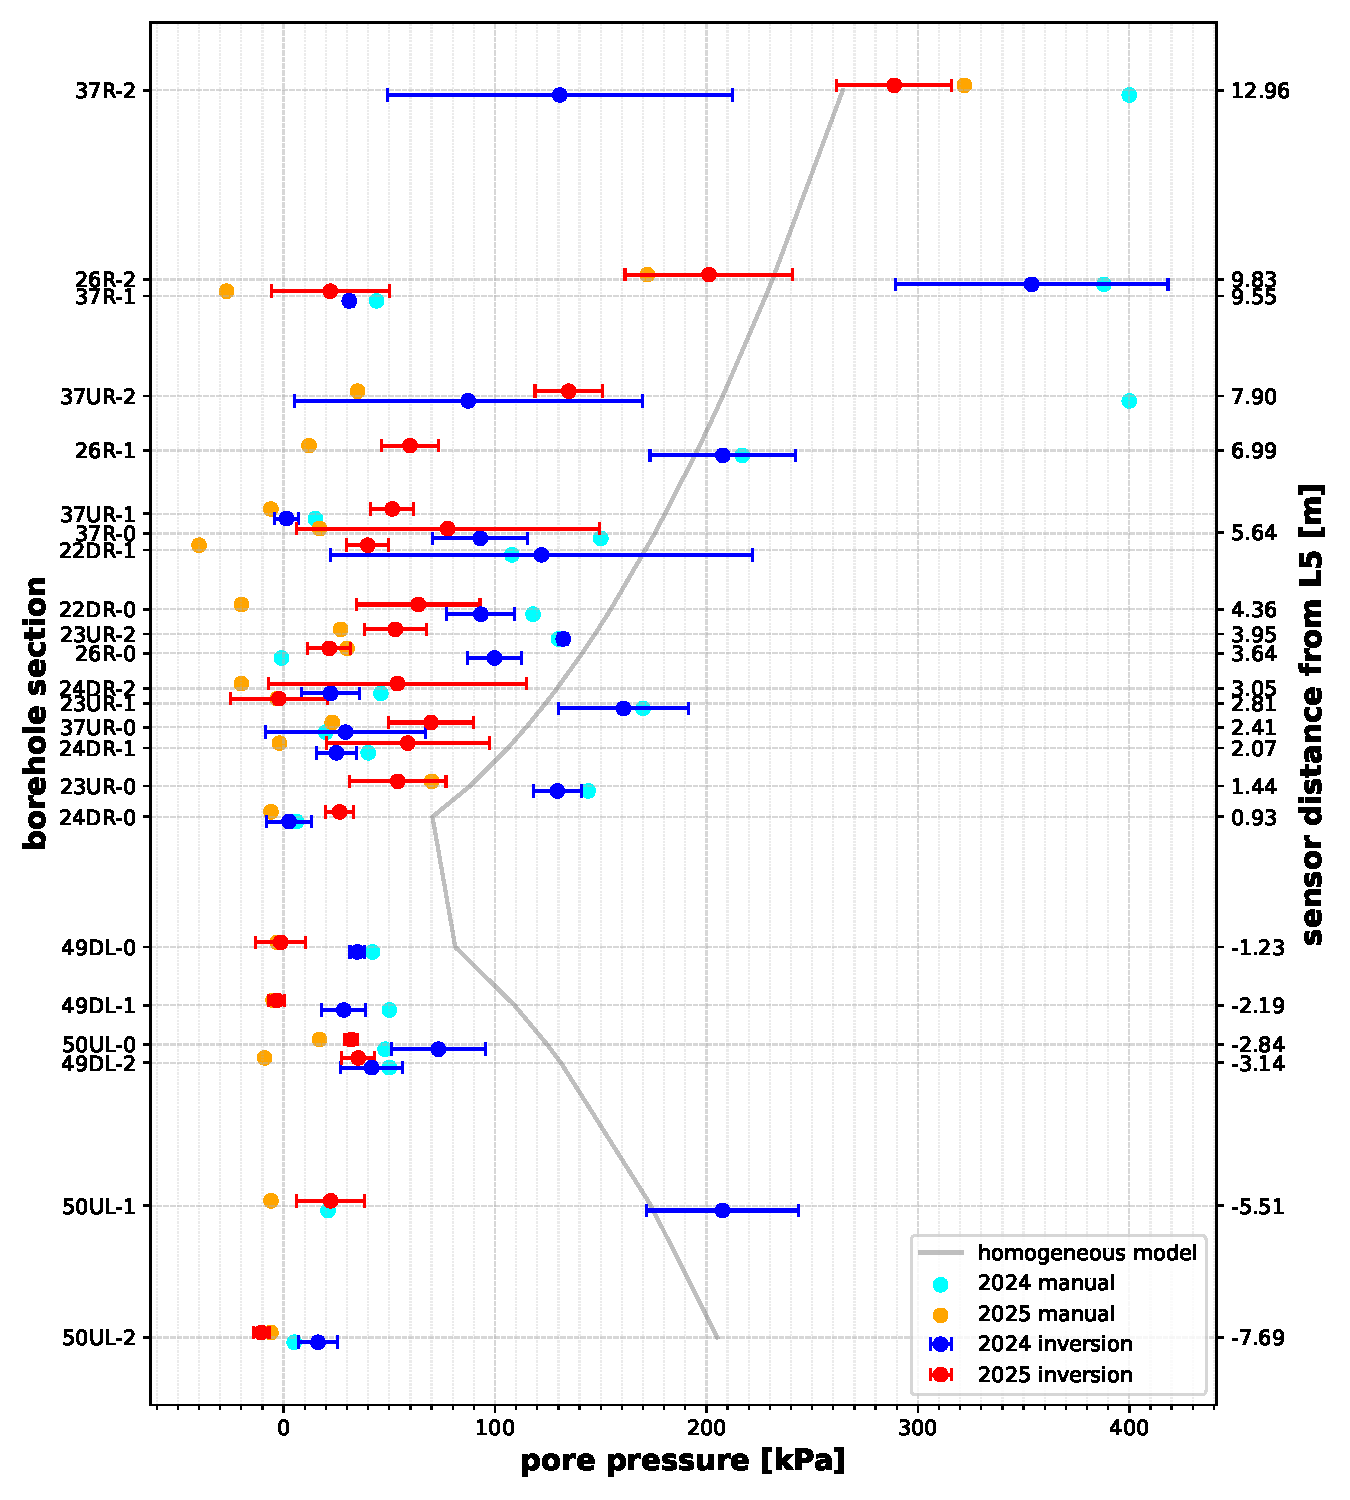
\includegraphics[width=\linewidth]{PP_figs/pressure_summary.pdf}
    \caption{Equilibrium pore pressure measured and extrapolated from Bayesian inversion.}
    \label{fig:pressure_summary}
  \end{subfigure}
  \hfill
  \begin{subfigure}[t]{0.49\textwidth}
    \centering
    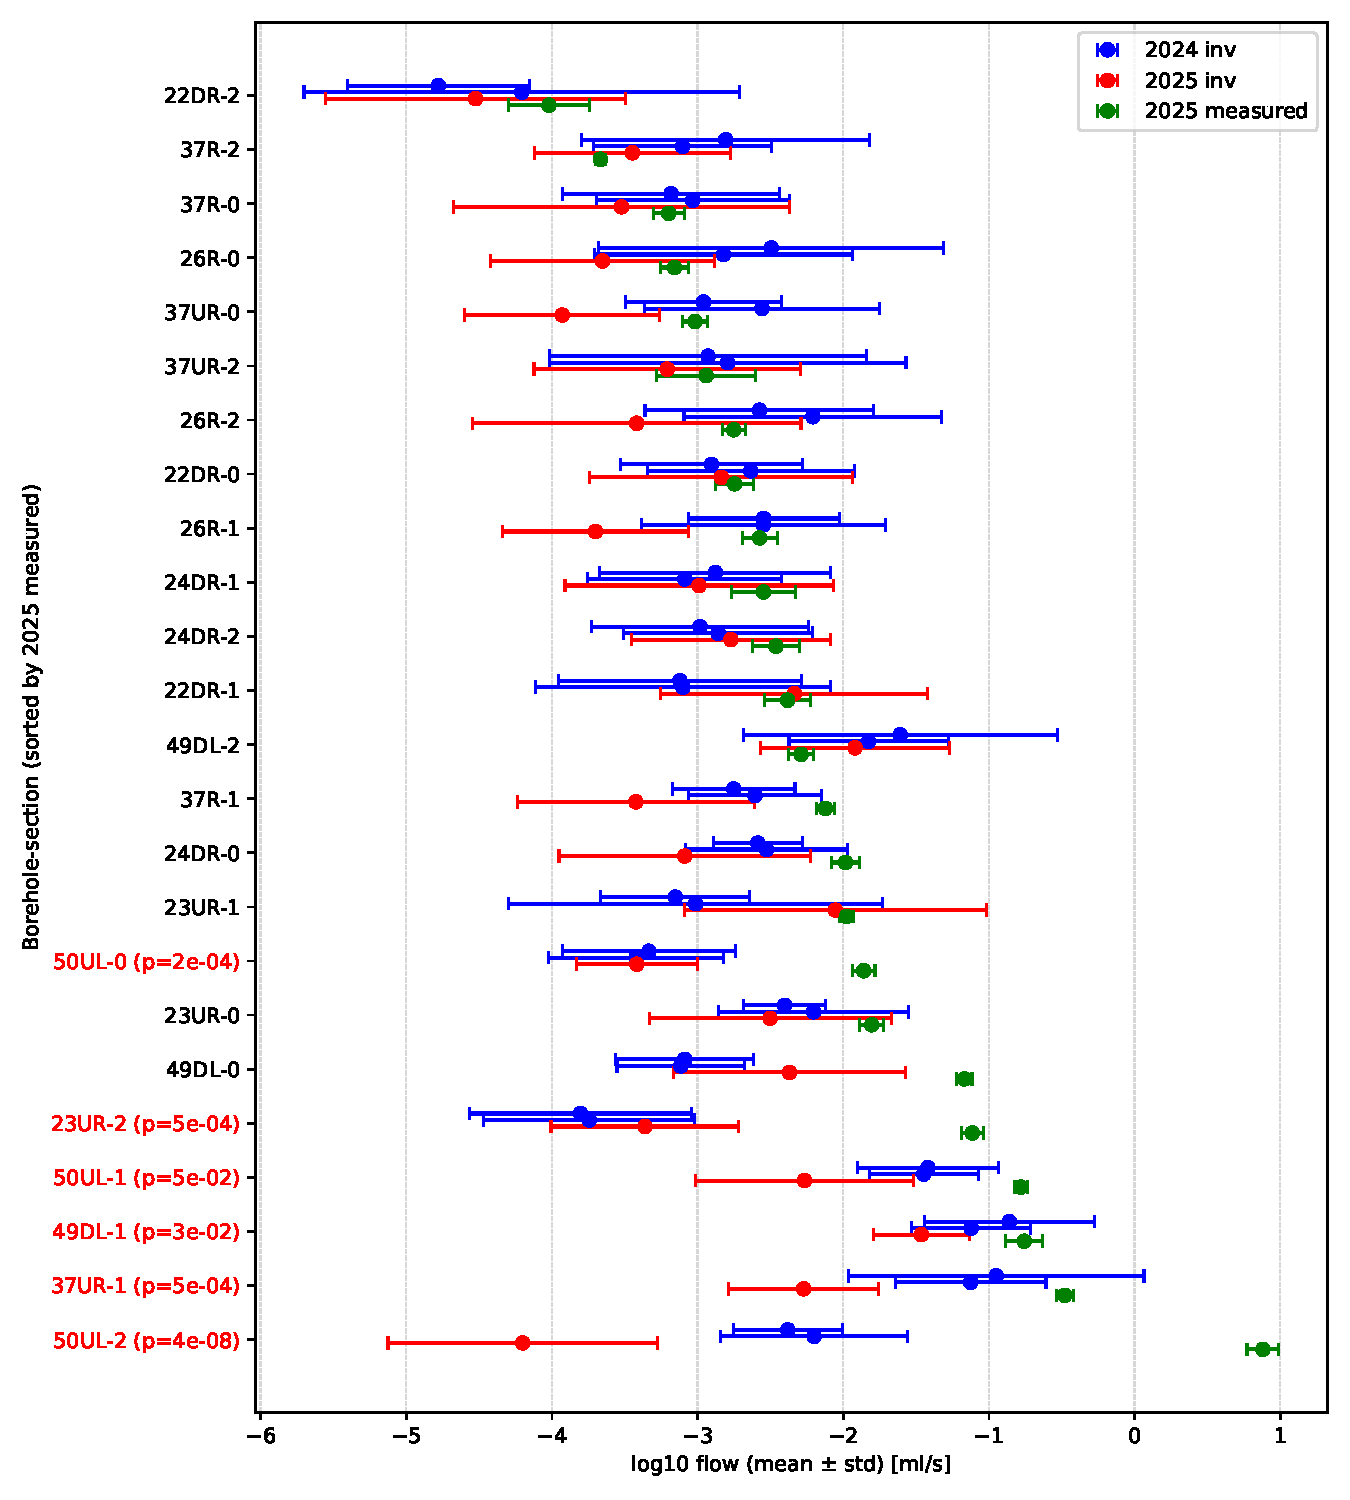
\includegraphics[width=\linewidth]{PP_figs/flow_summary.pdf}
    \caption{Measured and estimated water flux at the WPT peak pressure.}
    \label{fig:flow_summary}
  \end{subfigure}

  \caption{Equilibrium pore pressures (left) and water flux before (2024) and after excavation (2025), measured and extrapolated from Bayesian inversion.}
  \label{fig:flow_two_panel}
\end{figure}

\begin{figure}
    \begin{center}
    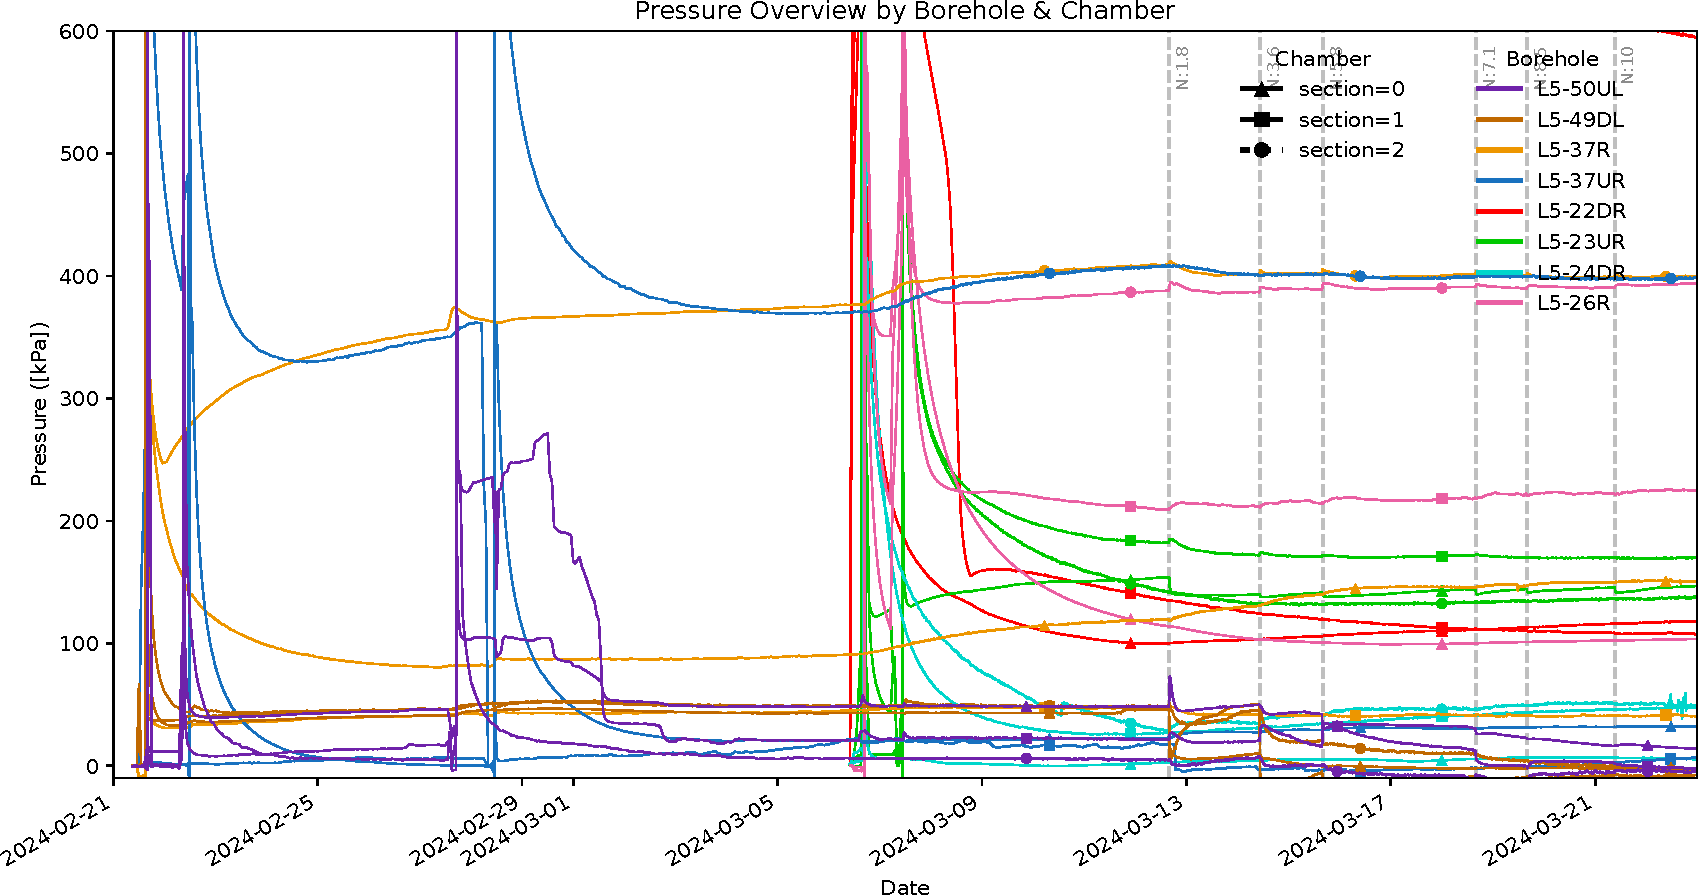
\includegraphics[width=\textwidth]{PP_figs/init_wpts_crop.pdf}
    \end{center}
    \caption{Pressure readings during initial water pressure tests in 2024. }
    \label{fig:init_wpts}
\end{figure}


% Group 1 ======================================================================
\FloatBarrier
\newpage

% \sts{[Nektere z nize popsanych vysledku a obrazku bych doporucil presunout do Apendixu uvedeneho na konci zaverecne zpravy. Text mi zde prijde prilis zdlouhavy.]}

\subsubsection{22DR-2}
This borehole cell exhibits an exceptionally slow pressure decrease. The initial short, rapid decay is followed by a long, almost linear decrease in pressure
(Fig. \ref{fig:wpts_cases_01_06}). This indicates that the measured cell is connected to a local fracture that is separated from a more conductive
zone (or the excavation) by compact rock. Note that a linear decrease corresponds to the 1D Darcy problem, while the kernel solution is $p(t) \sim -\ln(t)$
for the 2D case and $p(t) \sim t^{-1}$ for the 3D case. Thus, flow through the compact rock has an almost 1D character, so the boundary of the inner,
unconnected fracture is either short or remains at an almost constant distance from the target, more conductive zone. The much shorter initial decay
for both WPTs following the excavation may be caused by closure of the inner fracture, or more likely by its partial desaturation due to drilling of the measurement borehole.
The Bayesian inversion (Fig. \ref{fig:bayes_22DR_2}), as well as the comparison of the WPT curves
(Fig. \ref{fig:wpts_cases_01_06}), indicates an increase in the equilibrium pressure, but the uncertainty is rather high.


\subsubsection{37UR-2}
Two pressurizations were conducted before the excavation, both with rapid decay toward the pressure curve of \region{37R-2}, indicating a
possible connection (Fig. \ref{fig:init_wpts}). Moreover, a mild but significant pressure rise is observed after the WPTs in boreholes
\region{22DR} and \region{23UR}. The same pattern appears in \region{37R-2} and, at lower pressure levels, also in \region{37R-0} and \region{23UR-0}. Moreover, similar response to the north blasts appears in \region{37UR-2} and \region{26R-2}.
The post-excavation WPTs (Fig. \ref{fig:wpts_cases_01_06}), as well as the inversion (Fig. \ref{fig:bayes_37UR_2}),
suggest no change in conductivity or stiffness, only a drop in the equilibrium pressure.

\subsubsection{26R-2}
The readings exhibit a similar reaction to the north blasts as in \region{37R-2}, and the pre-excavation pressure level was also similar.
The reaction to the excavation was the largest observed, followed by a substantial drop in the equilibrium pressure
(Fig. \ref{fig:wpts_cases_01_06}). Although the last WPT exhibits a slightly slower pressure decrease, the inversion
(Fig. \ref{fig:bayes_37UR_2}) suggests no change in conductivity or stiffness.

\subsubsection{26R-1}
The initial WPT shows no anomalies. Excavation causes a substantial drop in the equilibrium pressure, and we observe slower decay during both
post-excavation WPTs (Fig. \ref{fig:wpts_cases_01_06}). The inversion points to possibly decreased stiffness
(Fig. \ref{fig:bayes_37UR_2}).

\subsubsection{37R-2}
The response to the initial WPT is anomalous (Fig. \ref{fig:wpts_cases_01_06}): the initial pressure drop is followed by a substantial rise in pressure
that is not associated with any perturbation. A plausible explanation is rapid filling of a drained fracture, allowing an initial pressure decrease and subsequent
recovery toward an equilibrium pressure that seems to be largely preserved after excavation. The equilibrium pressure appears to be unaffected by the excavation,
and the long-term behavior exhibits a kind of seasonal variability. Surprisingly, the 1D model with an almost constant initial pressure $p_R$ was able to fit this
non-monotone behavior, at the cost of unrealistic conductivity values and large stiffness heterogeneity (Fig. \ref{fig:bayes_37UR_2}).
% \jb{TODO: inspect evolution of the best fit simulation}

\subsubsection{37R-0}
There is a slight pressure increase in reaction to the second WPT in \region{37UR} (Fig. \ref{fig:wpts_cases_01_06}), which, together with other similarities,
suggests a weak connection. The sustained tendency of increasing pressure before and during the early phase of excavation, together with the very smooth long-term evolution,
is consistent with the idea of a relatively large fracture weakly communicating with the new excavation. A large fracture area helps to smooth out disturbances.
The much faster pressure relaxation after the first WPT could be partially caused by drainage after borehole drilling. The inversion (Fig. \ref{fig:bayes_37R_0})
also suggests a slight increase in conductivity. This could be compatible with the expected decrease in compressive stress on the lateral sides of the excavation
and the implied fracture opening.
\newpage
\begin{figure}[H]
    \begin{center}
    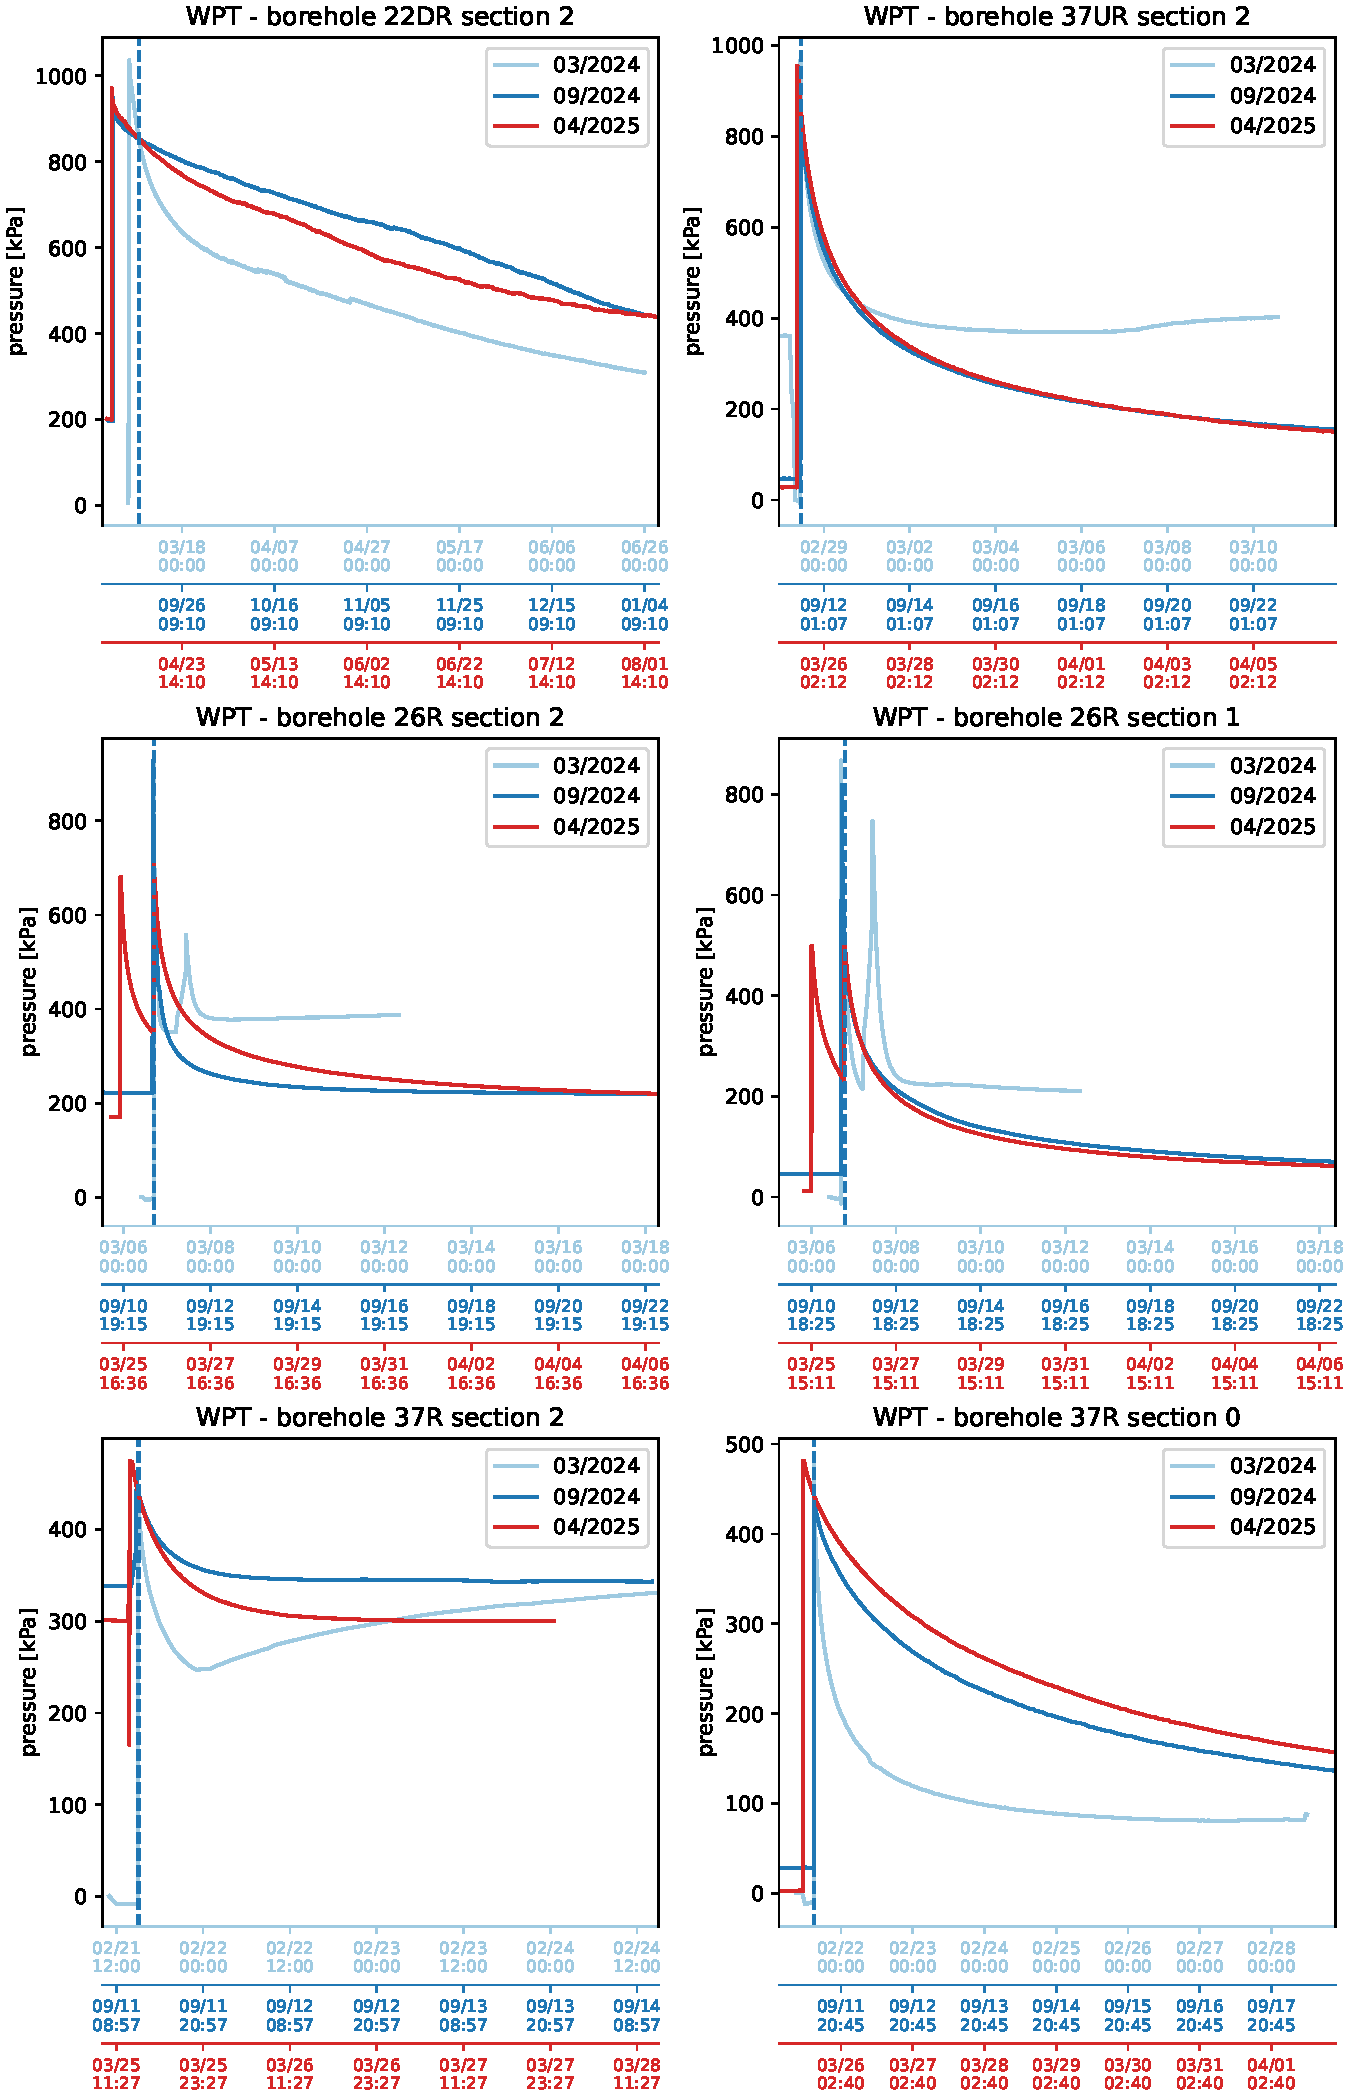
\includegraphics[width=0.9\textwidth]{PP_figs/wpt_grid_01.pdf}
    \end{center}
    \caption{Stitched water pressure test plots.}
    \label{fig:wpts_cases_01_06}
\end{figure}
\FloatBarrier
\newpage
\begin{figure}
    \begin{center}
    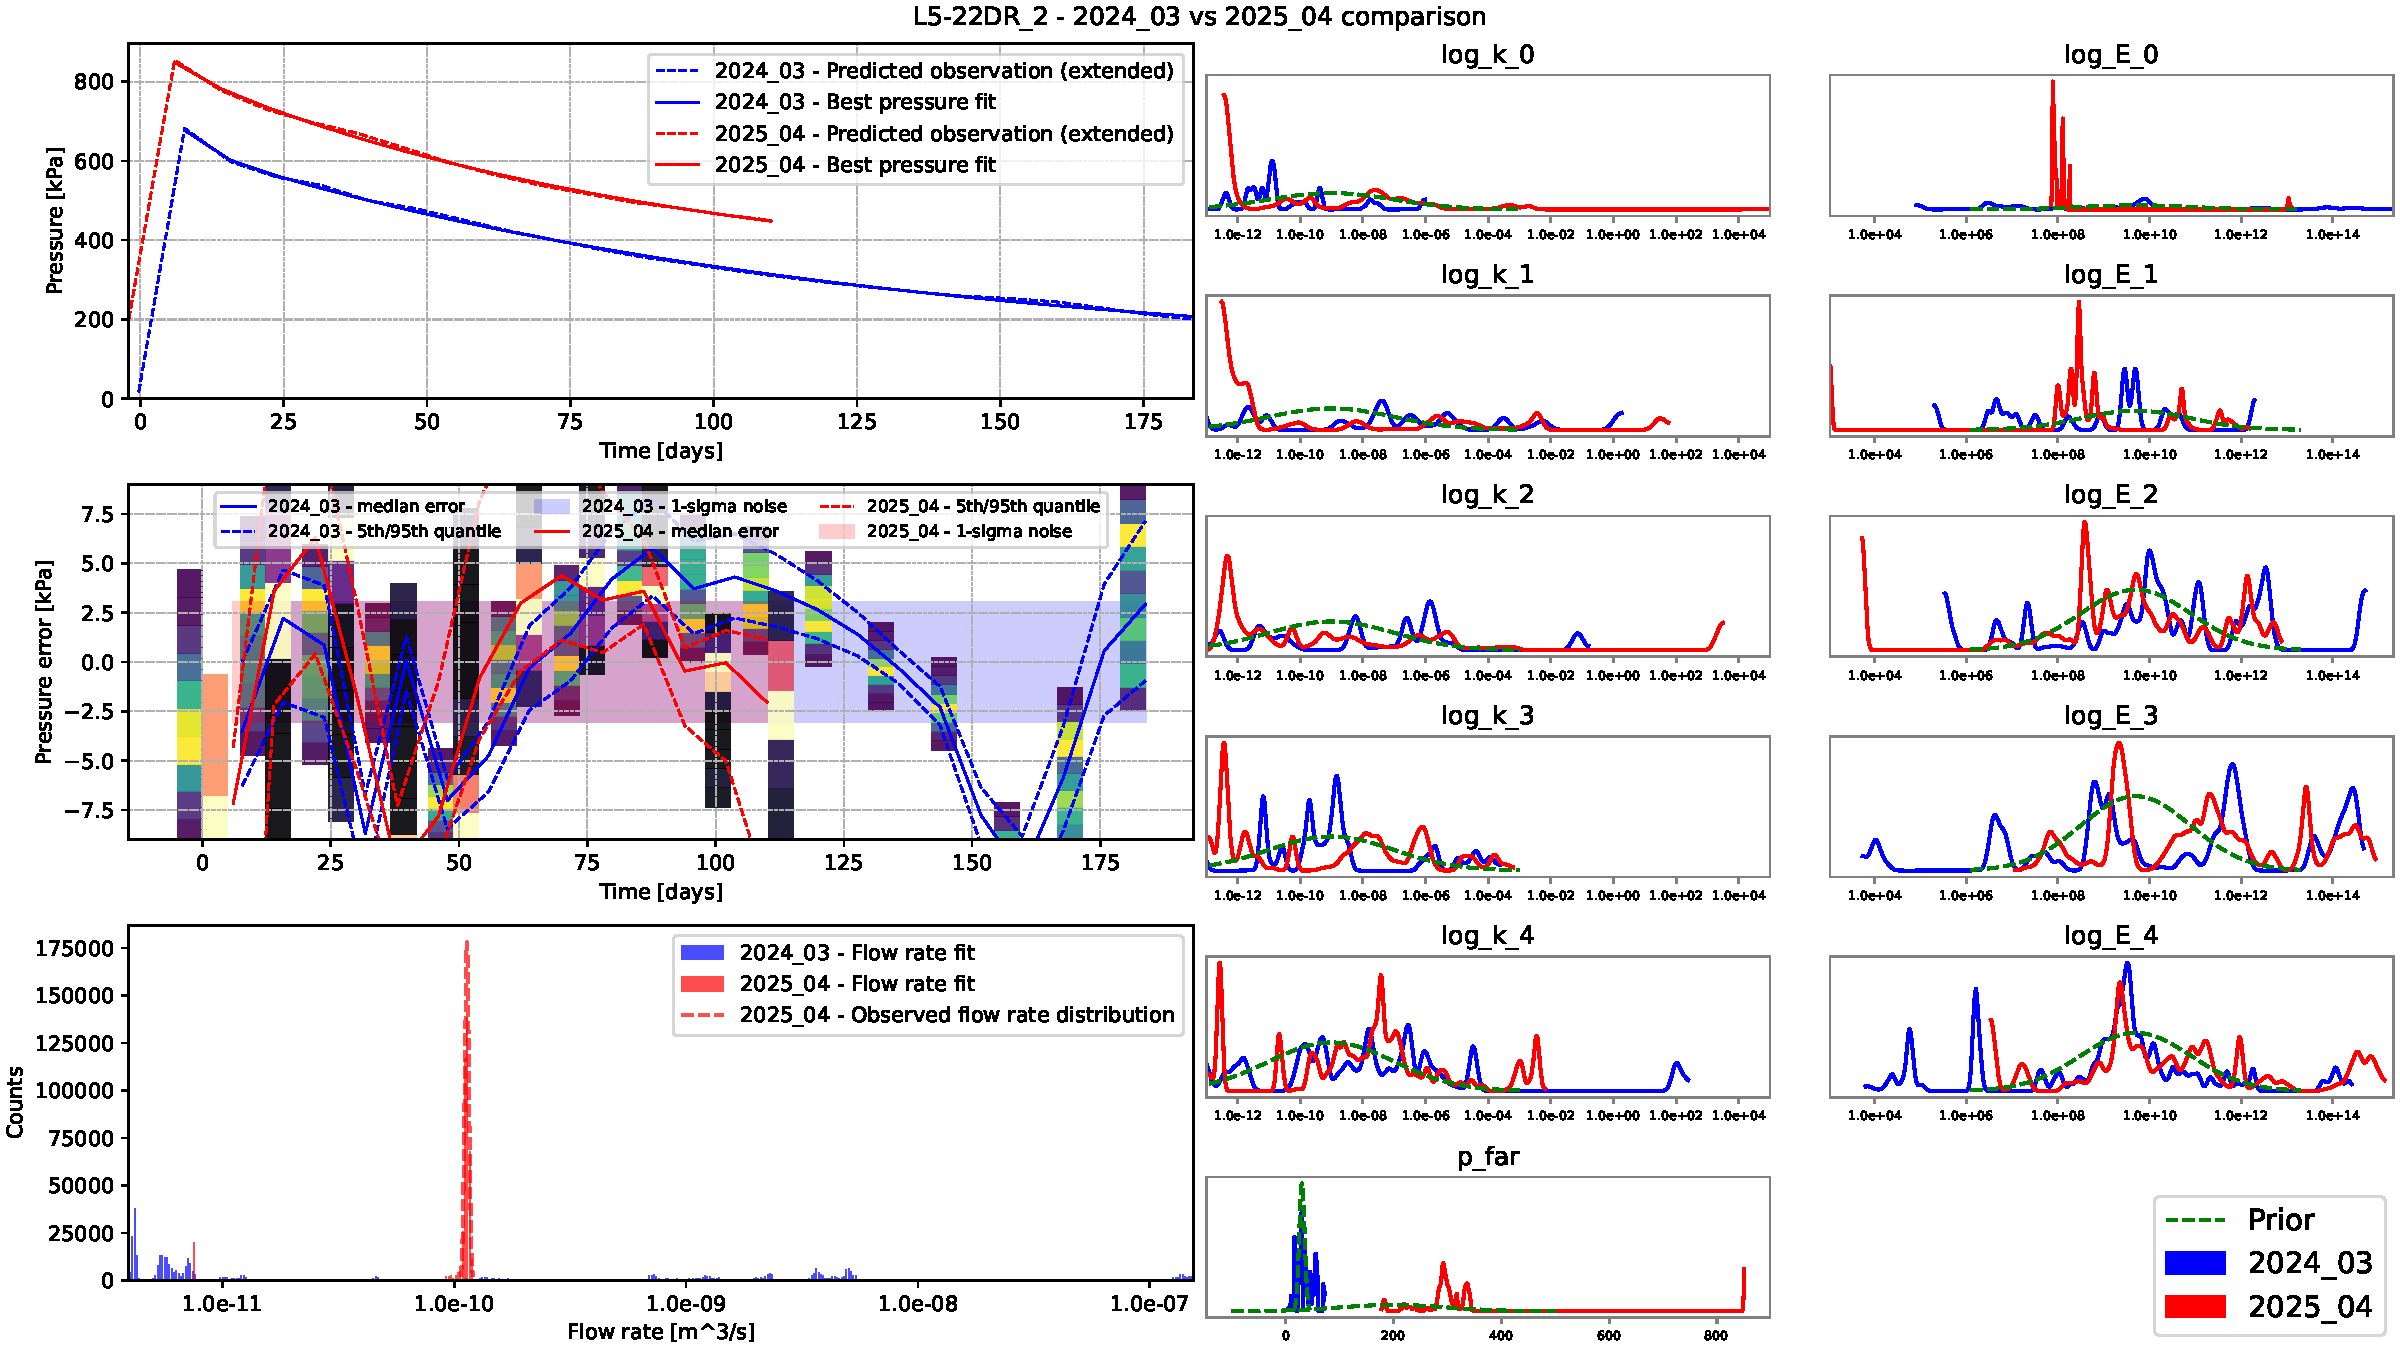
\includegraphics[width=0.8\textwidth]{PP_figs/22DR_2_compareplot.pdf}
    \end{center}
    \caption{Bayesian inversion summary for cell 22DR-2.}
    \label{fig:bayes_22DR_2}
\end{figure}
\begin{figure}
    \begin{center}
    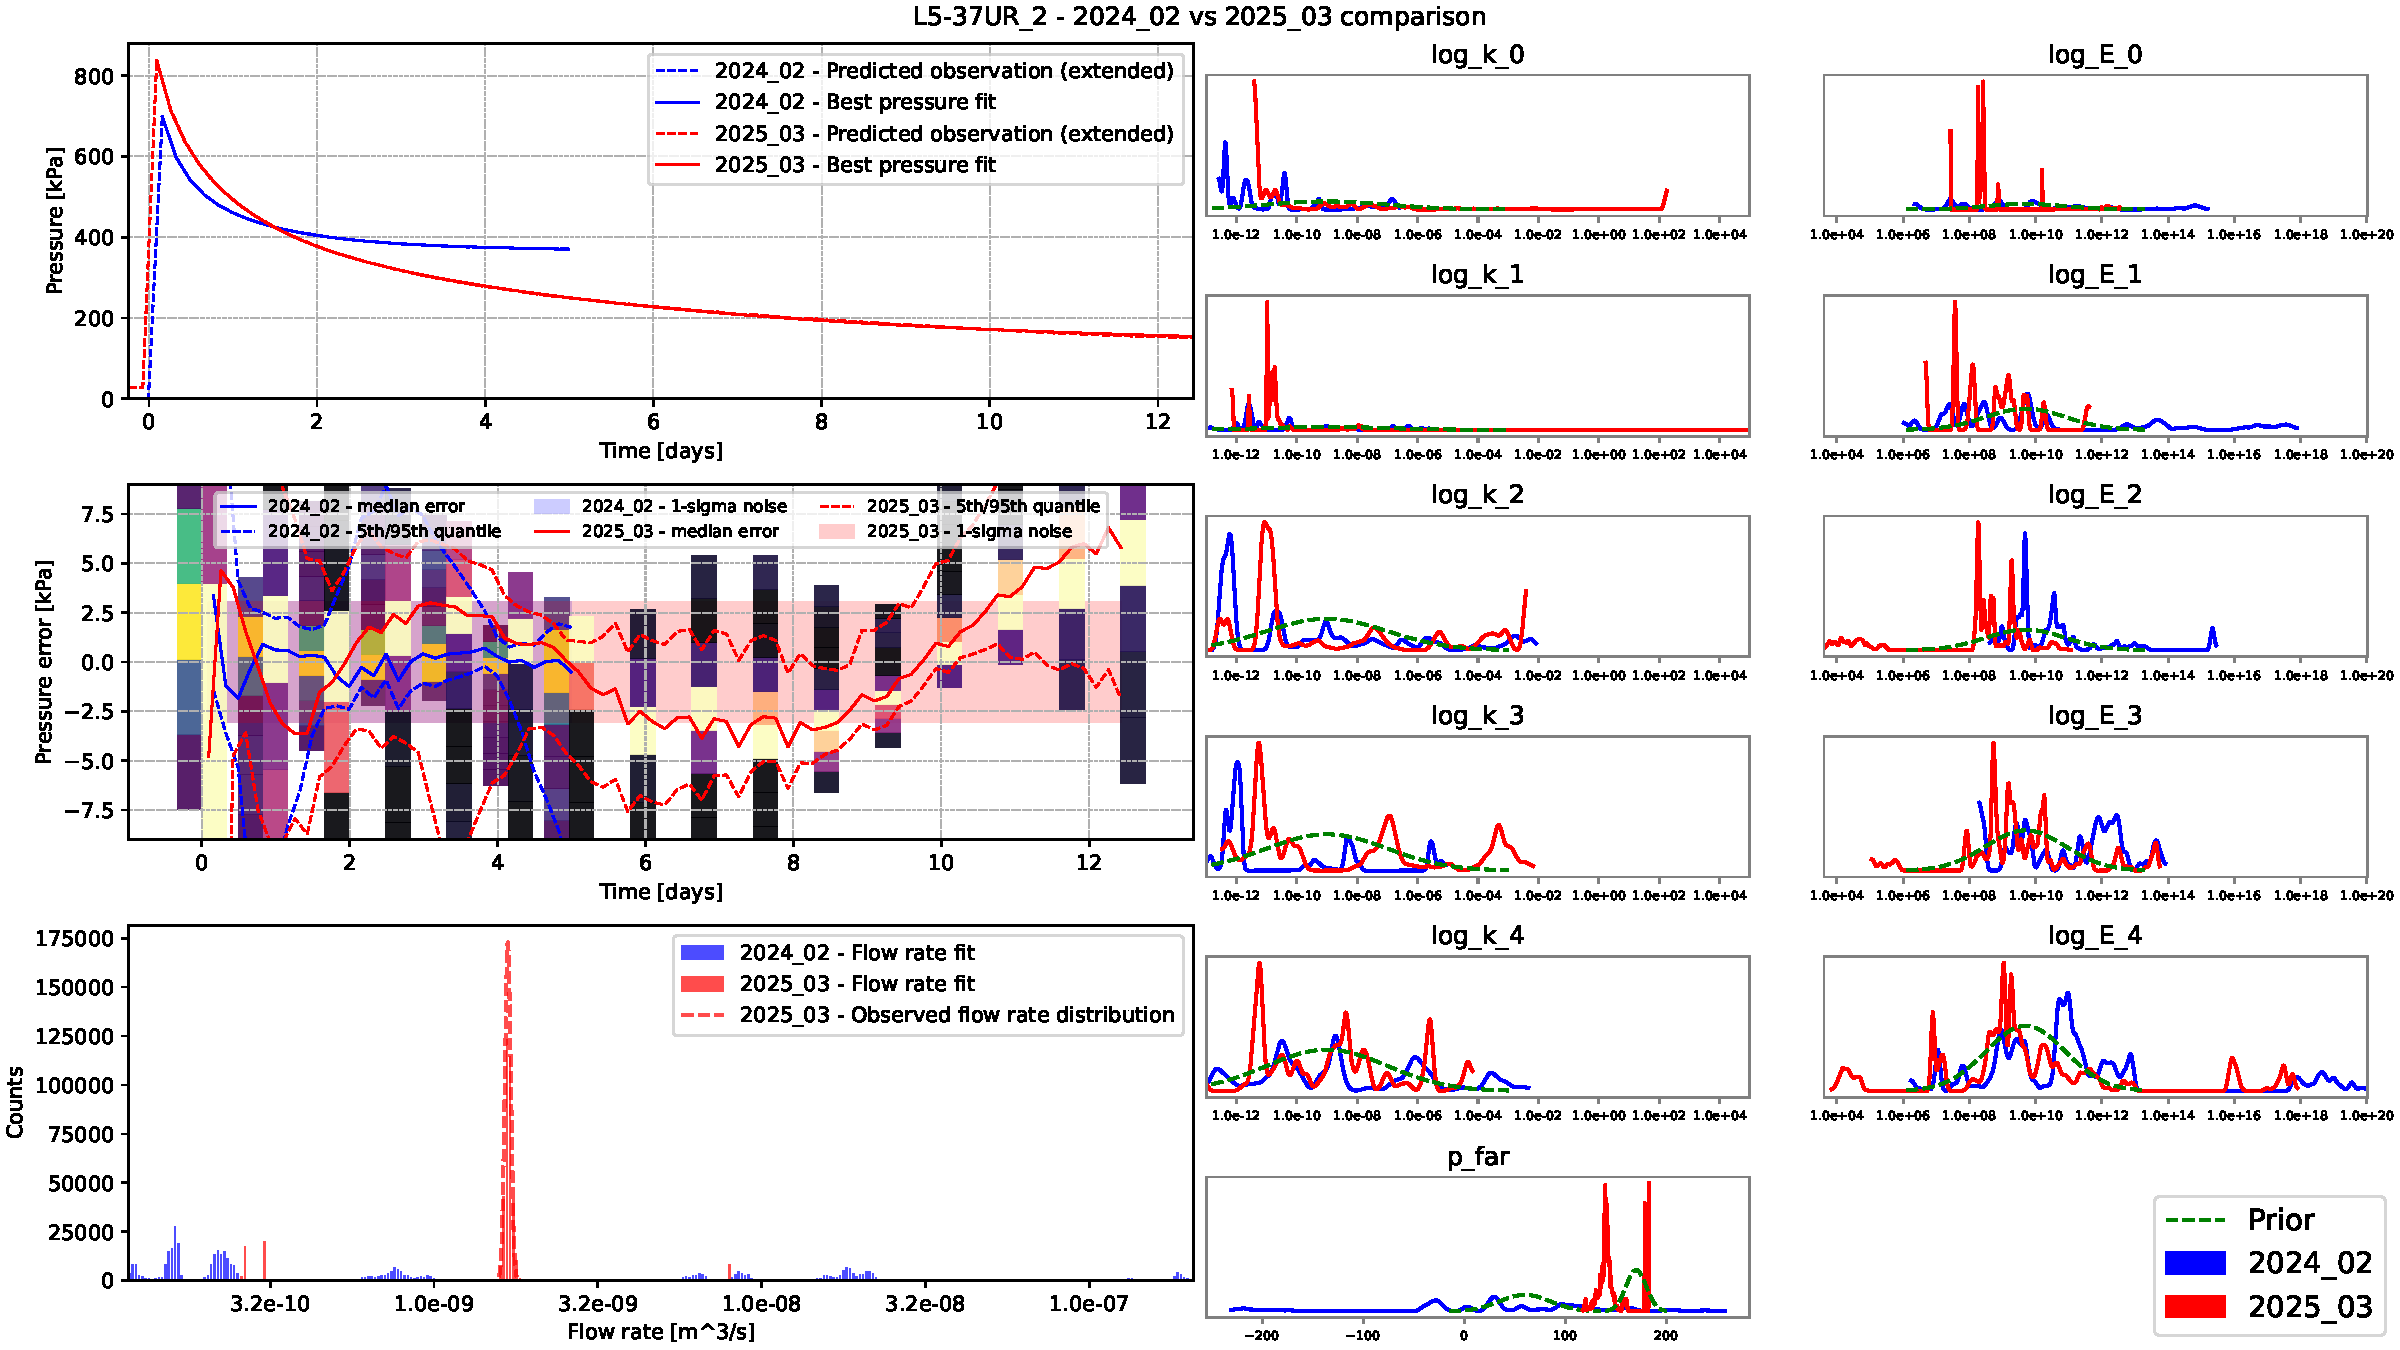
\includegraphics[width=0.8\textwidth]{PP_figs/37UR_2_compareplot.pdf}
    \end{center}
    \caption{Bayesian inversion summary for cell 37UR-2.}
    \label{fig:bayes_37UR_2}
\end{figure}
\begin{figure}
    \begin{center}
    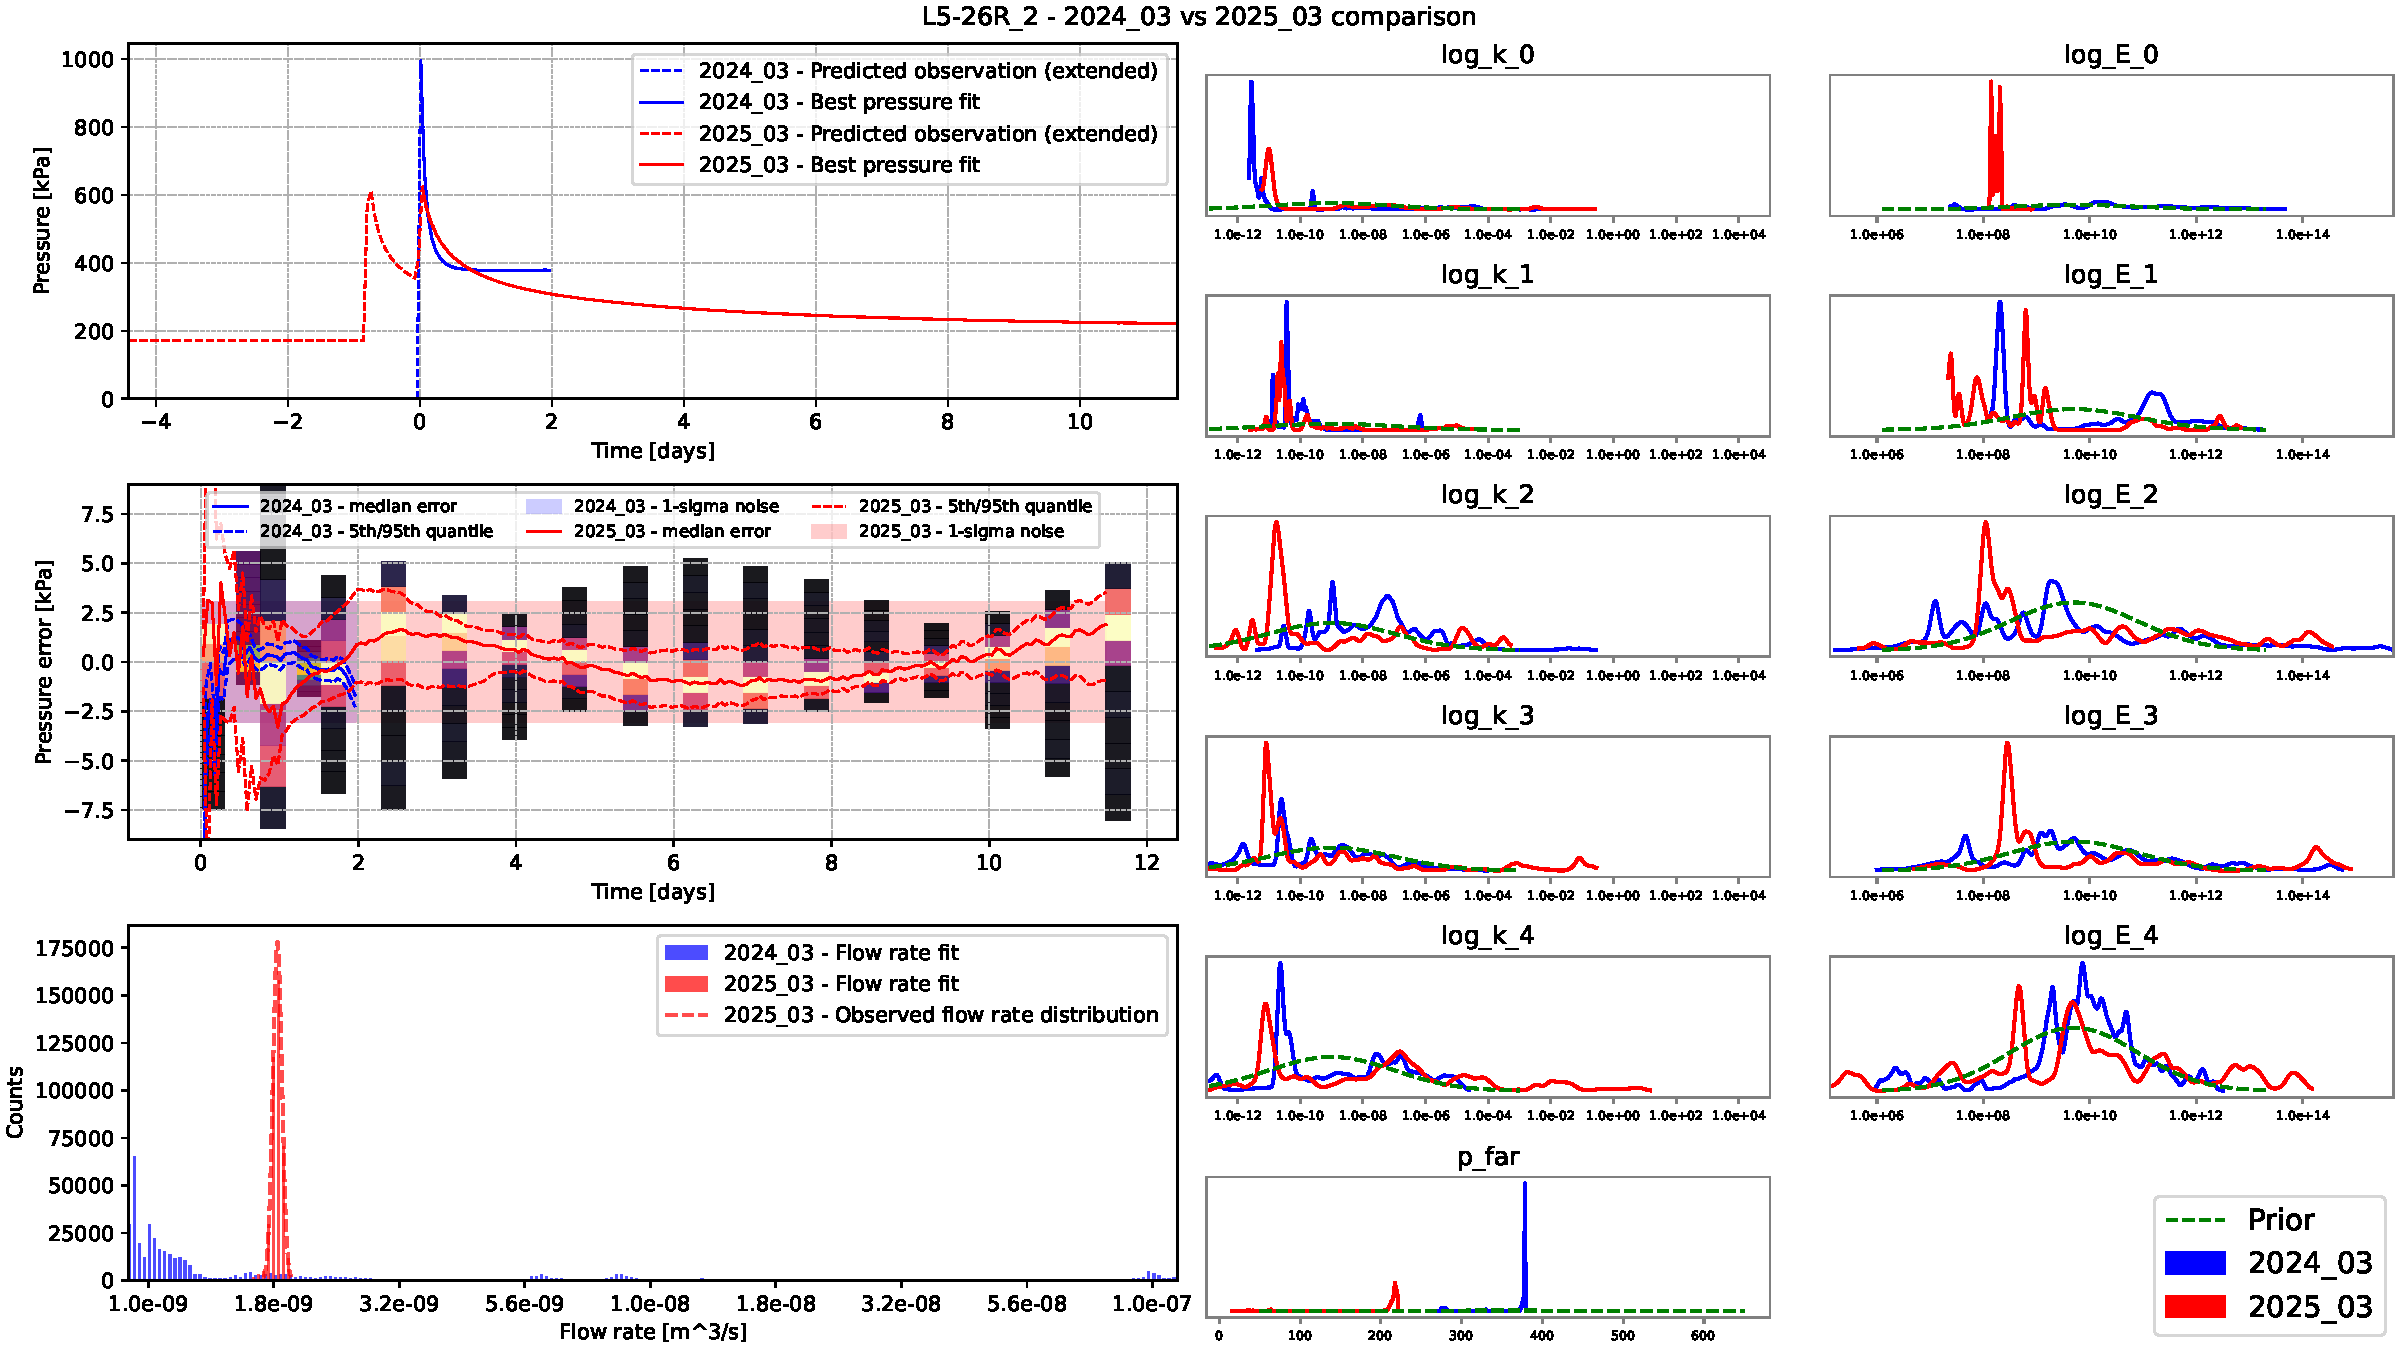
\includegraphics[width=0.75\textwidth]{PP_figs/26R_2_compareplot.pdf}
    \end{center}
    \caption{Bayesian inversion summary for cell 26R-2.}
    \label{fig:bayes_26R_2}
\end{figure}
\FloatBarrier
\newpage
\begin{figure}
    \begin{center}
    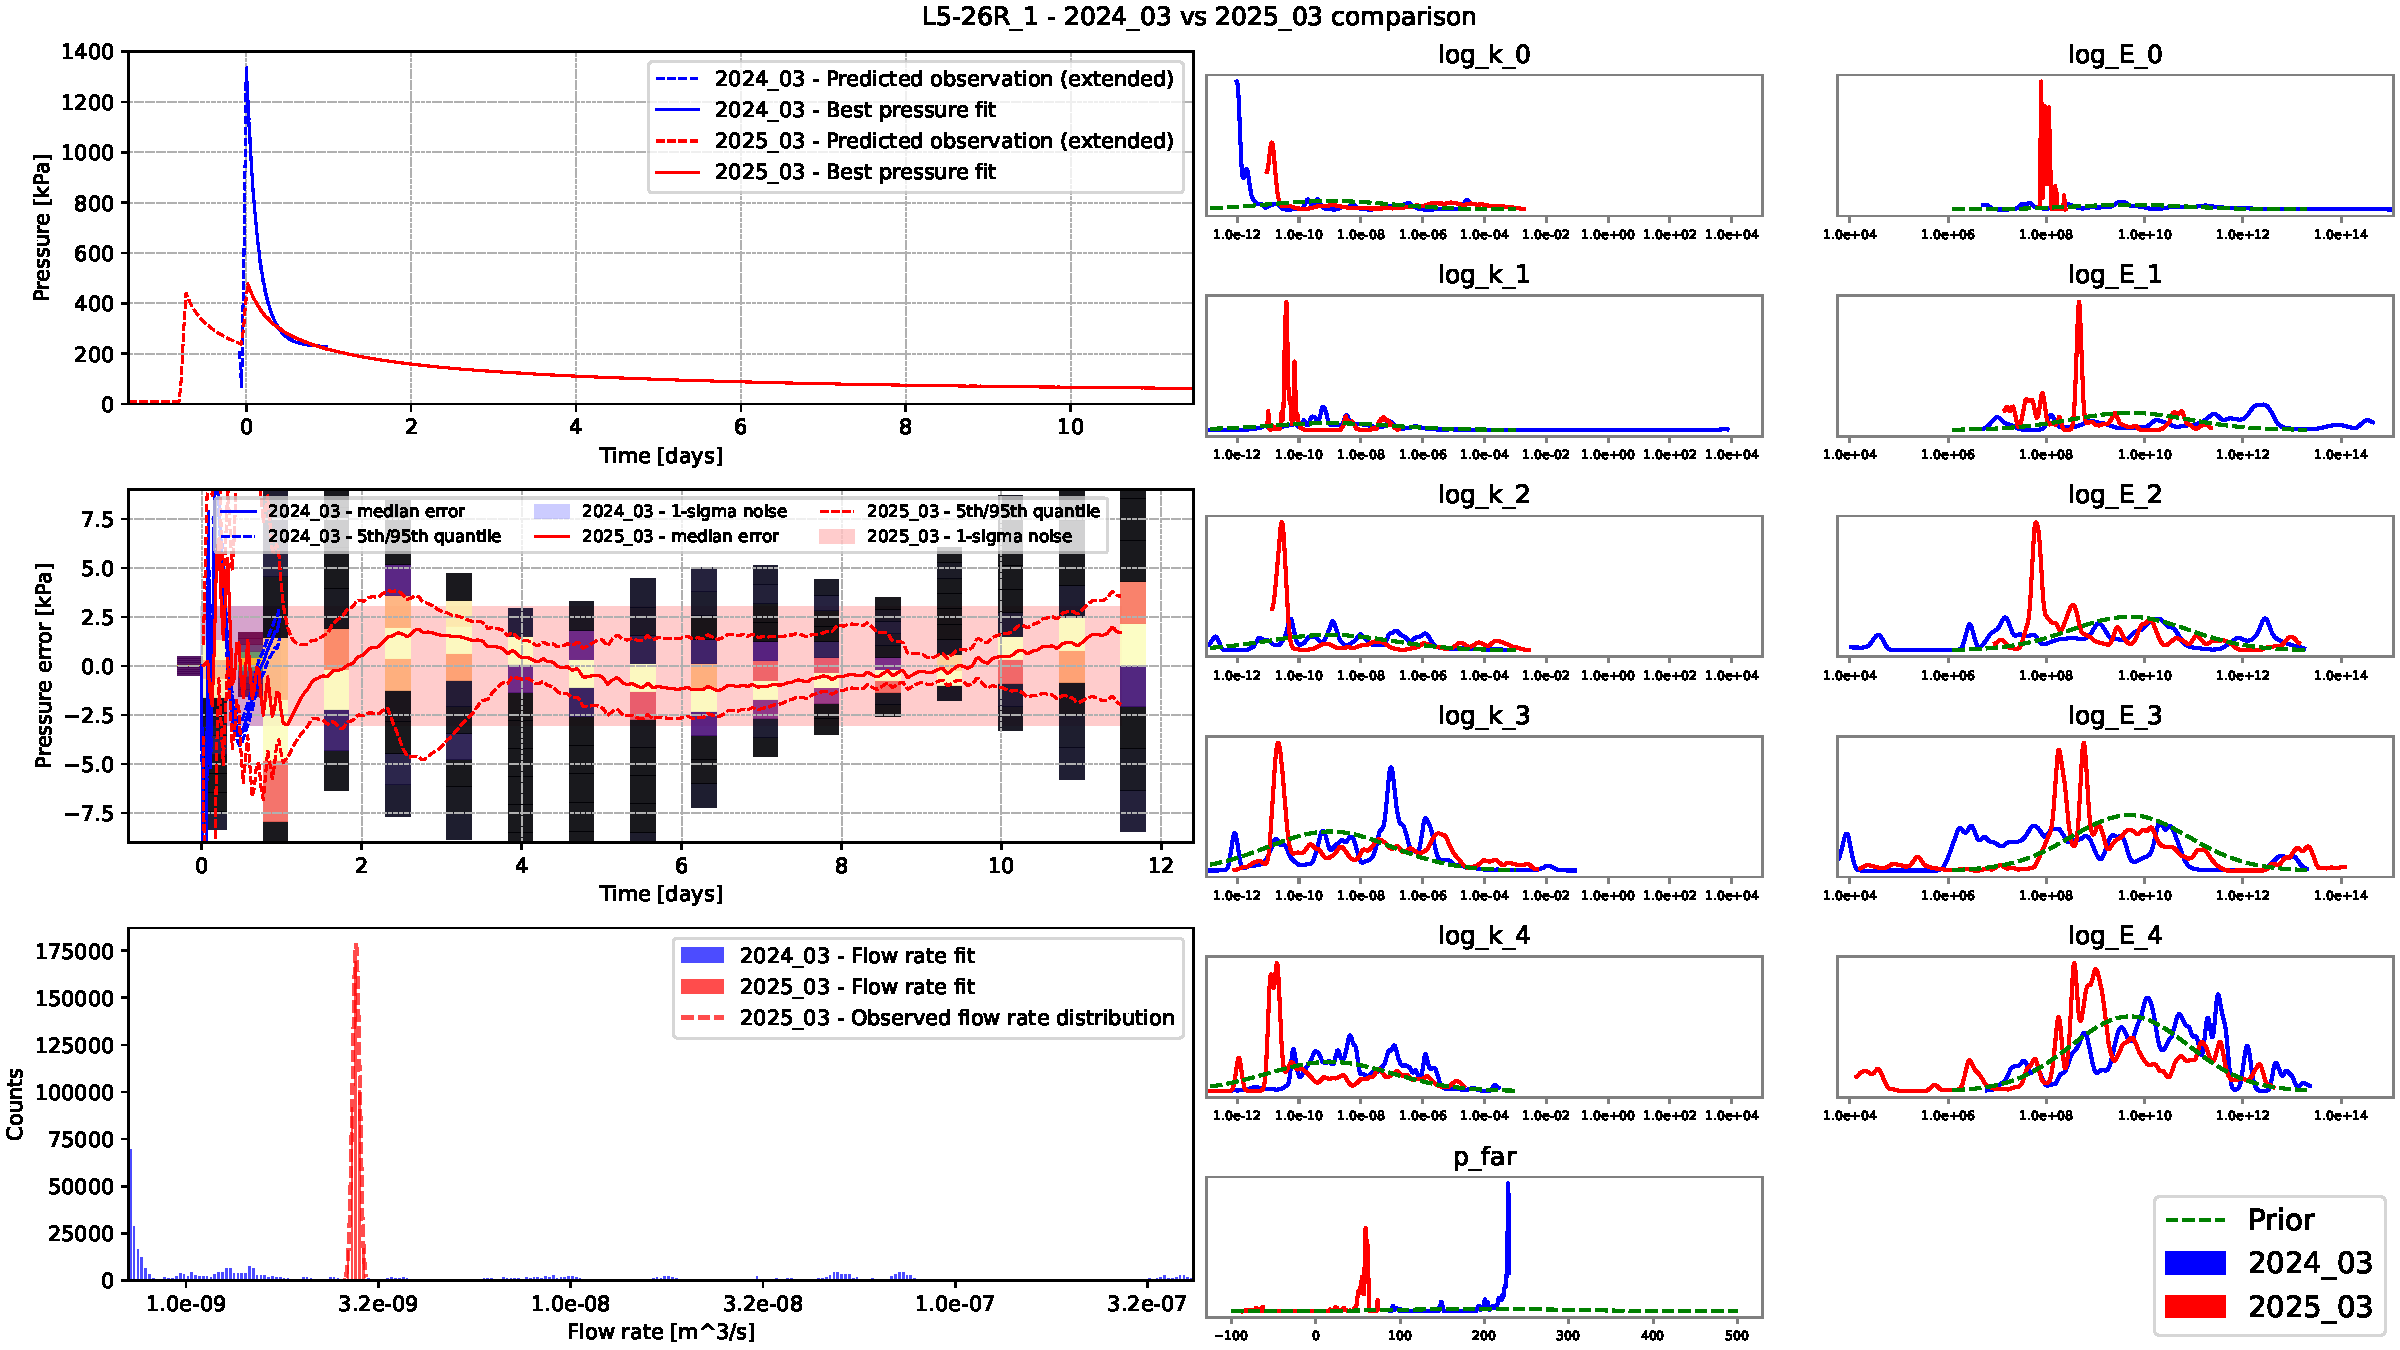
\includegraphics[width=0.75\textwidth]{PP_figs/26R_1_compareplot.pdf}
    \end{center}
    \caption{Bayesian inversion summary for cell 26R-1.}
    \label{fig:bayes_26R_1}
\end{figure}
\begin{figure}
    \begin{center}
    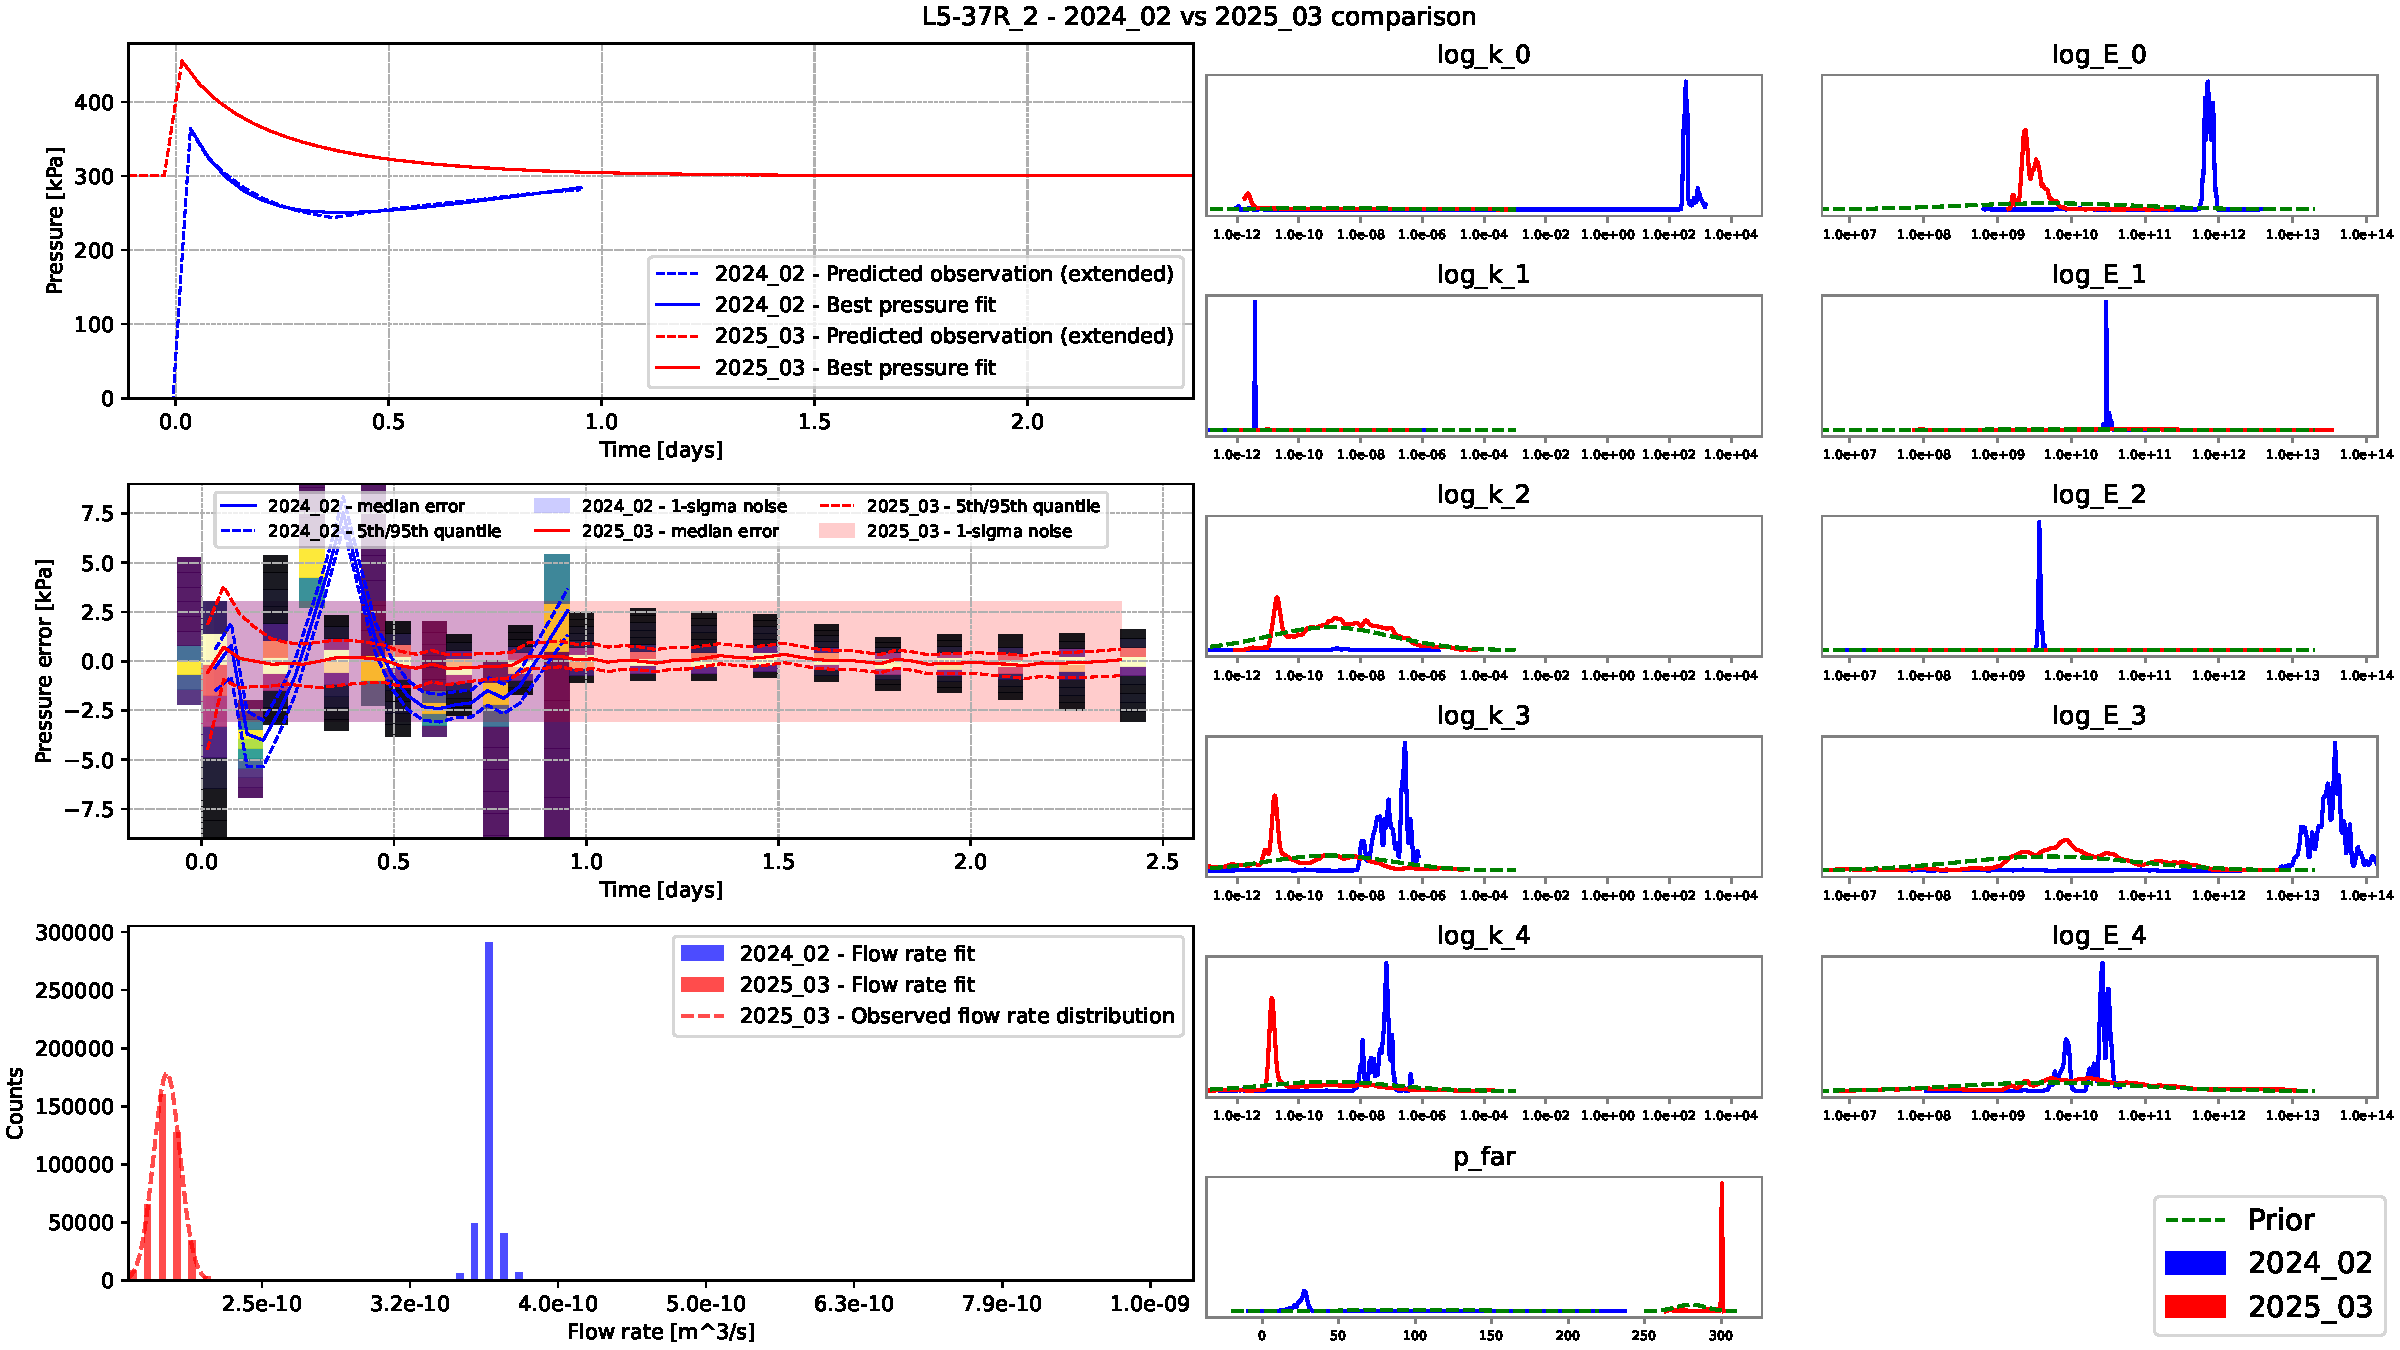
\includegraphics[width=0.75\textwidth]{PP_figs/37R_2_compareplot.pdf}
    \end{center}
    \caption{Bayesian inversion summary for cell 37R-2.}
    \label{fig:bayes_37R_2}
\end{figure}
\begin{figure}
    \begin{center}
    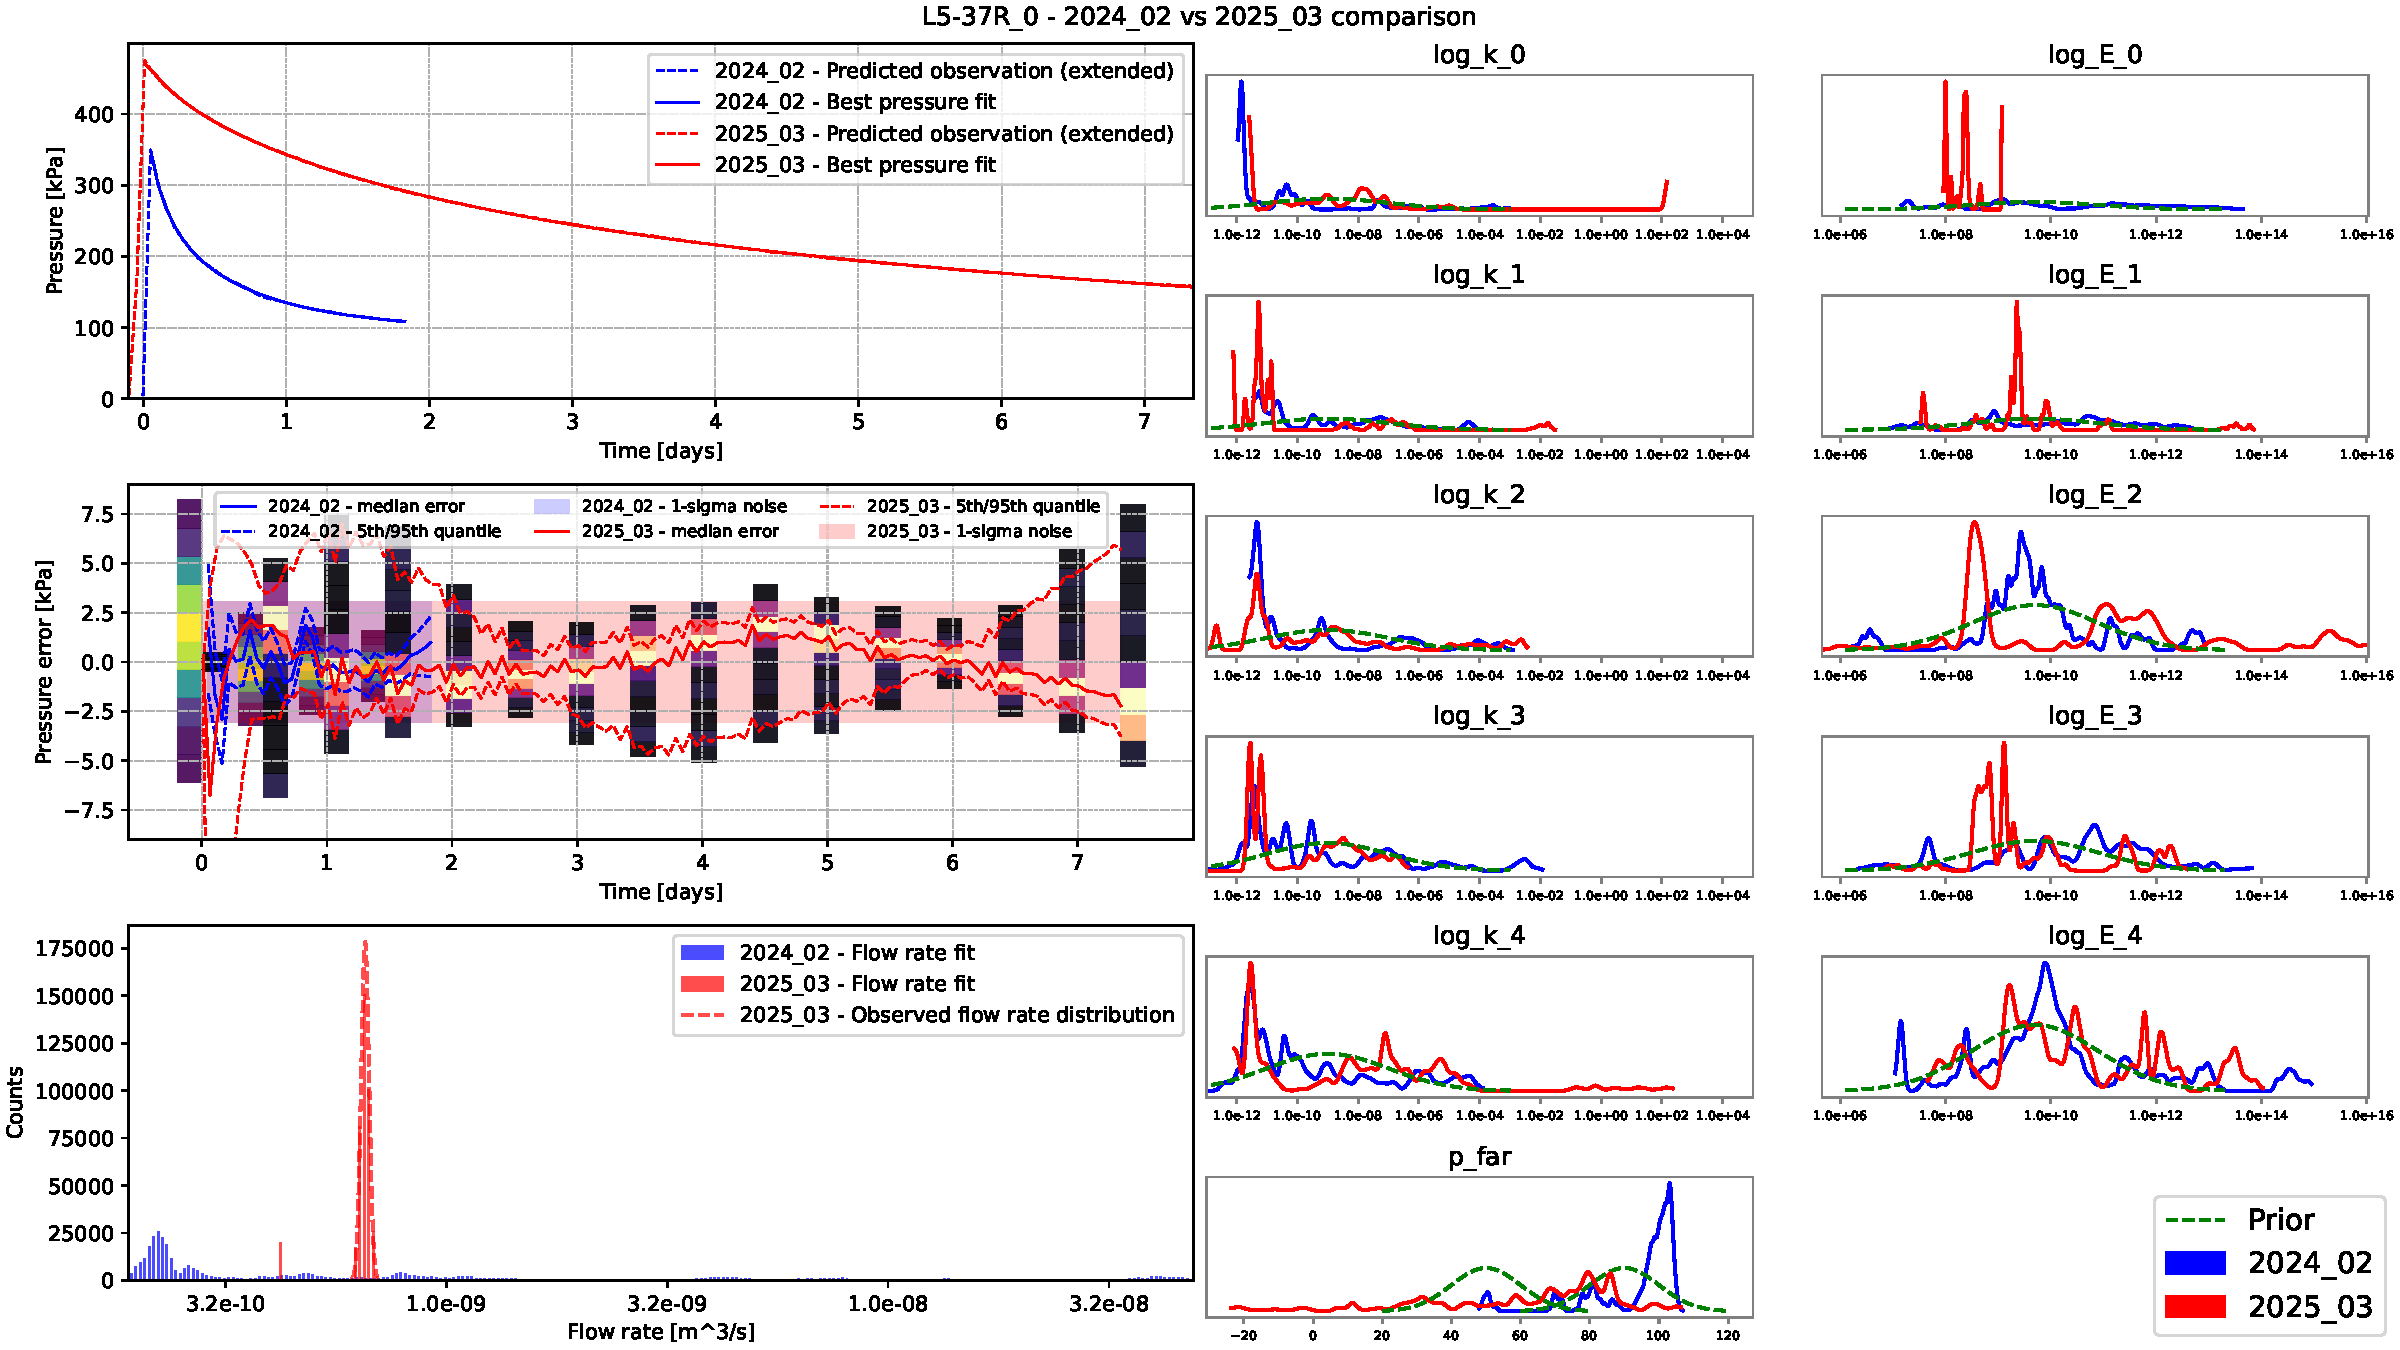
\includegraphics[width=0.75\textwidth]{PP_figs/37R_0_compareplot.pdf}
    \end{center}
    \caption{Bayesian inversion summary for cell 37R-0.}
    \label{fig:bayes_37R_0}
\end{figure}
\FloatBarrier
\newpage
% Group 2 ======================================================================
\subsubsection{23UR-0}
The response to the initial WPT (Fig. \ref{fig:init_wpts}) exhibits a
similar drop--raise pattern as in \region{37R-2}, but with a shape similar
to \region{37R-0}. The sensor shows a pressure-drop response to the north
blast events, unique among the south sensors. While the response appears
to be an instantaneous pressure drop, it is in fact a classical
exponential transition to a lower pressure over about 1--2 hours after
the blast, pointing to a slight change in the stress field close to the
sensor. The south blasts cause a much more dramatic pressure drop, but
the long-term post-excavation trend is still increasing, reaching the new
equilibrium by the time of the second round of WPTs, about 7 months after the
excavation. The immediate WPT response (Fig. \ref{fig:wpts_cases_07_012})
does not change, and the inversion does not suggest any change in
material parameters.

\subsubsection{22DR-1}
Abnormal reaction to the first WPT (Fig. \ref{fig:wpts_cases_07_012}).
The initial pressure decrease was much slower than what was observed
after the excavation. However, after about two days, a pressure decrease
similar to the rate of the post-excavation WPTs was observed for about
10 hours. The trend then suddenly changed to a slow pressure increase,
which within about one day shifted to an even slower decrease that
continued up to the first south blast. This suggests activation of a
more conductive path that remains active after the excavation. A
substantial decrease in equilibrium pressure readings occur during
2025. The inversion (Fig. \ref{fig:bayes_22DR_1}) indicates a substantial
increase in conductivity in close to the sensor (about 1~m), consistent with
this activation explanation.

\subsubsection{23UR-1}
Small but significant reaction to the first 2--3 north blasts. During
the initial WPTs, there are many cross-reactions, but none were observed
during later WPTs; \region{23UR-1} is the only exception, exhibiting a pressure increase
in reaction to the 2025 WPT on \region{23UR-2}. The response to all WPTs
(Fig. \ref{fig:wpts_cases_07_012}) is consistent, with only a decreased
equilibrium pressure. The inversion (Fig. \ref{fig:bayes_23UR_1})
indicates increased conductivity and decreased stiffness; however, this
is more likely due to the true water flux measured in 2025 being
significantly higher than the predicted flux in 2024.

\subsubsection{26R-0}
No sudden events. The long-term pattern is a slow increase after
excavation until the second round of WPTs, followed by a much faster
long-term decay between the last two WPT rounds, and then a significant
pressure rise in mid-2025. This long-term pattern is similar to that of
\region{37R-1}. Comparison of WPTs (Fig. \ref{fig:wpts_cases_07_012})
indicates a small decrease in equilibrium pressure and a slightly slower
pressure decay in 2025. The inversion (Fig. \ref{fig:bayes_26R_0}),
however, shows no significant change in the material parameters.

\subsubsection{23UR-2}
After the initial WPT, the reading decays below \region{23UR-1} and even
below \region{23UR-0}. During the first month of 2025, a sawtooth pattern
appears on sensors \region{23UR-2}, \region{50UL-0}, and \region{50UL-1} in particular.
The sensor was destroyed on 2024/03/28 16:30 by
the third south blast, and later replaced by external measurement
through the pressurization tube. Comparison of WPTs
(Fig. \ref{fig:wpts_cases_07_012}) shows the same decay rate, but toward
a somewhat decreased equilibrium pressure. The change in material
parameters indicated by the inversion (Fig. \ref{fig:bayes_23UR_2}) is
most likely due to missing flow measurements and incorrect flow estimation in 2024.

\subsubsection{22DR-0}
The later two WPTs exhibit slower decay than the initial one
(Fig. \ref{fig:wpts_cases_07_012}), while the short-term equilibrium pressure is
unaffected. However, the long-term equilibrium pressure exhibits
remarkably large variations, in the range of about $-25$ to $25$~kPa
relative to the atmospheric pressure. The inversion
(Fig. \ref{fig:bayes_22DR_0}) indicates possibly decreased stiffness in
2025.
\newpage
\begin{figure}
    \begin{center}
    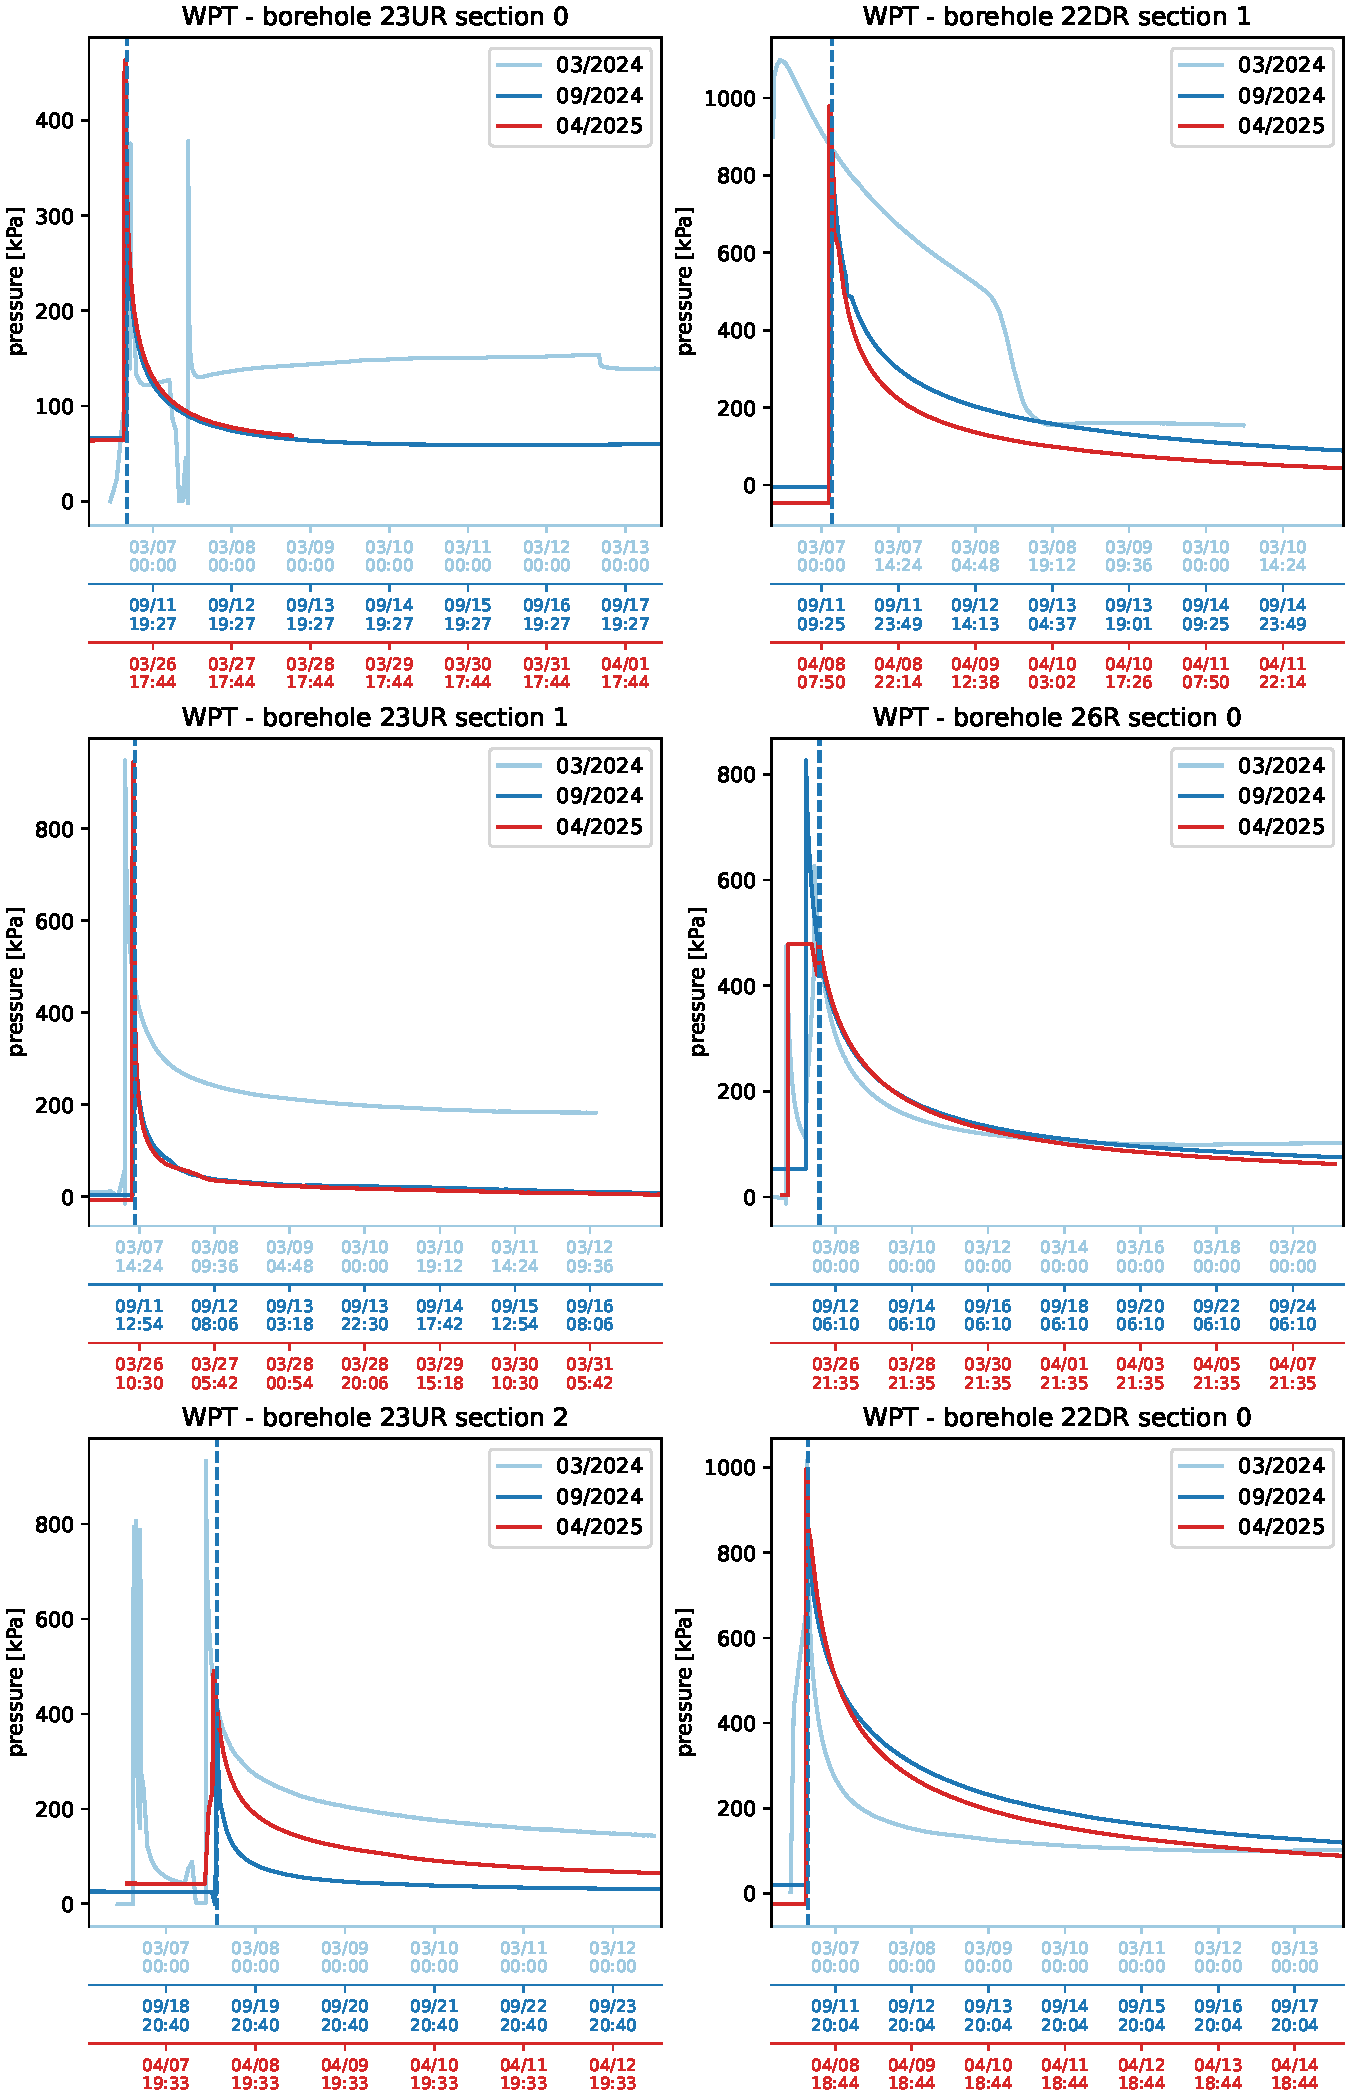
\includegraphics[width=0.9\textwidth]{PP_figs/wpt_grid_02.pdf}
    \end{center}
    \caption{Stitched water pressure test plots 02.}
    \label{fig:wpts_cases_07_012}
\end{figure}
\FloatBarrier
\newpage
\begin{figure}
    \begin{center}
    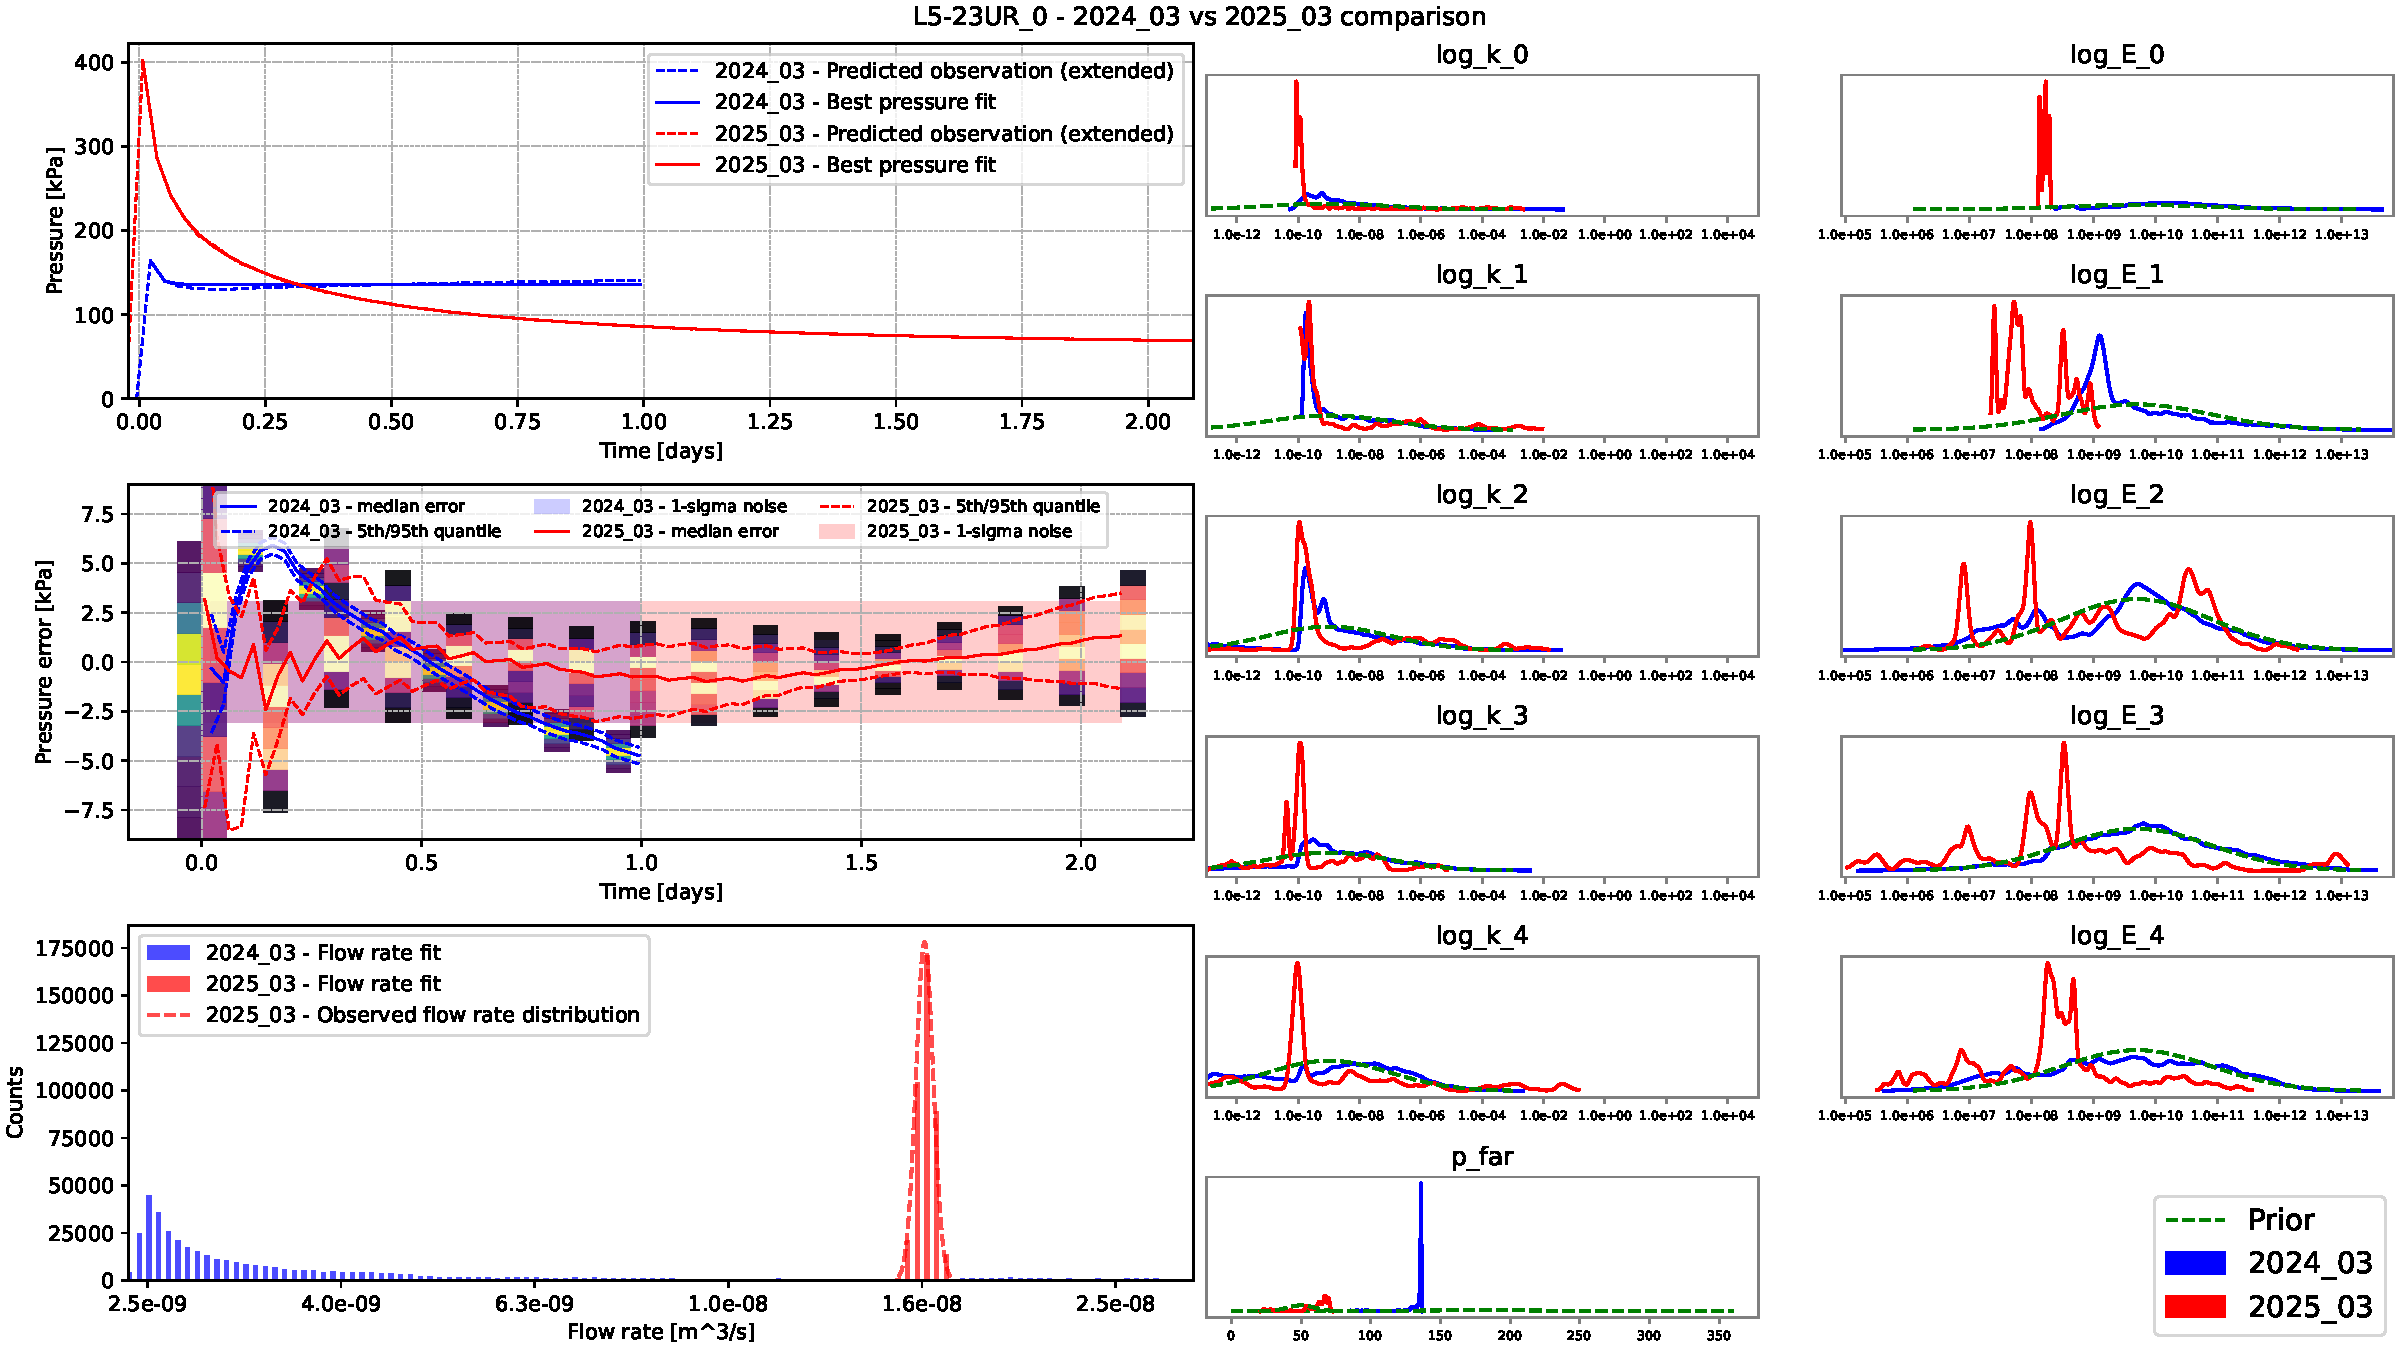
\includegraphics[width=0.75\textwidth]{PP_figs/23UR_0_compareplot.pdf}
    \end{center}
    \caption{Bayesian inversion summary for cell 23UR-0.}
    \label{fig:bayes_23UR_0}
\end{figure}
\begin{figure}
    \begin{center}
    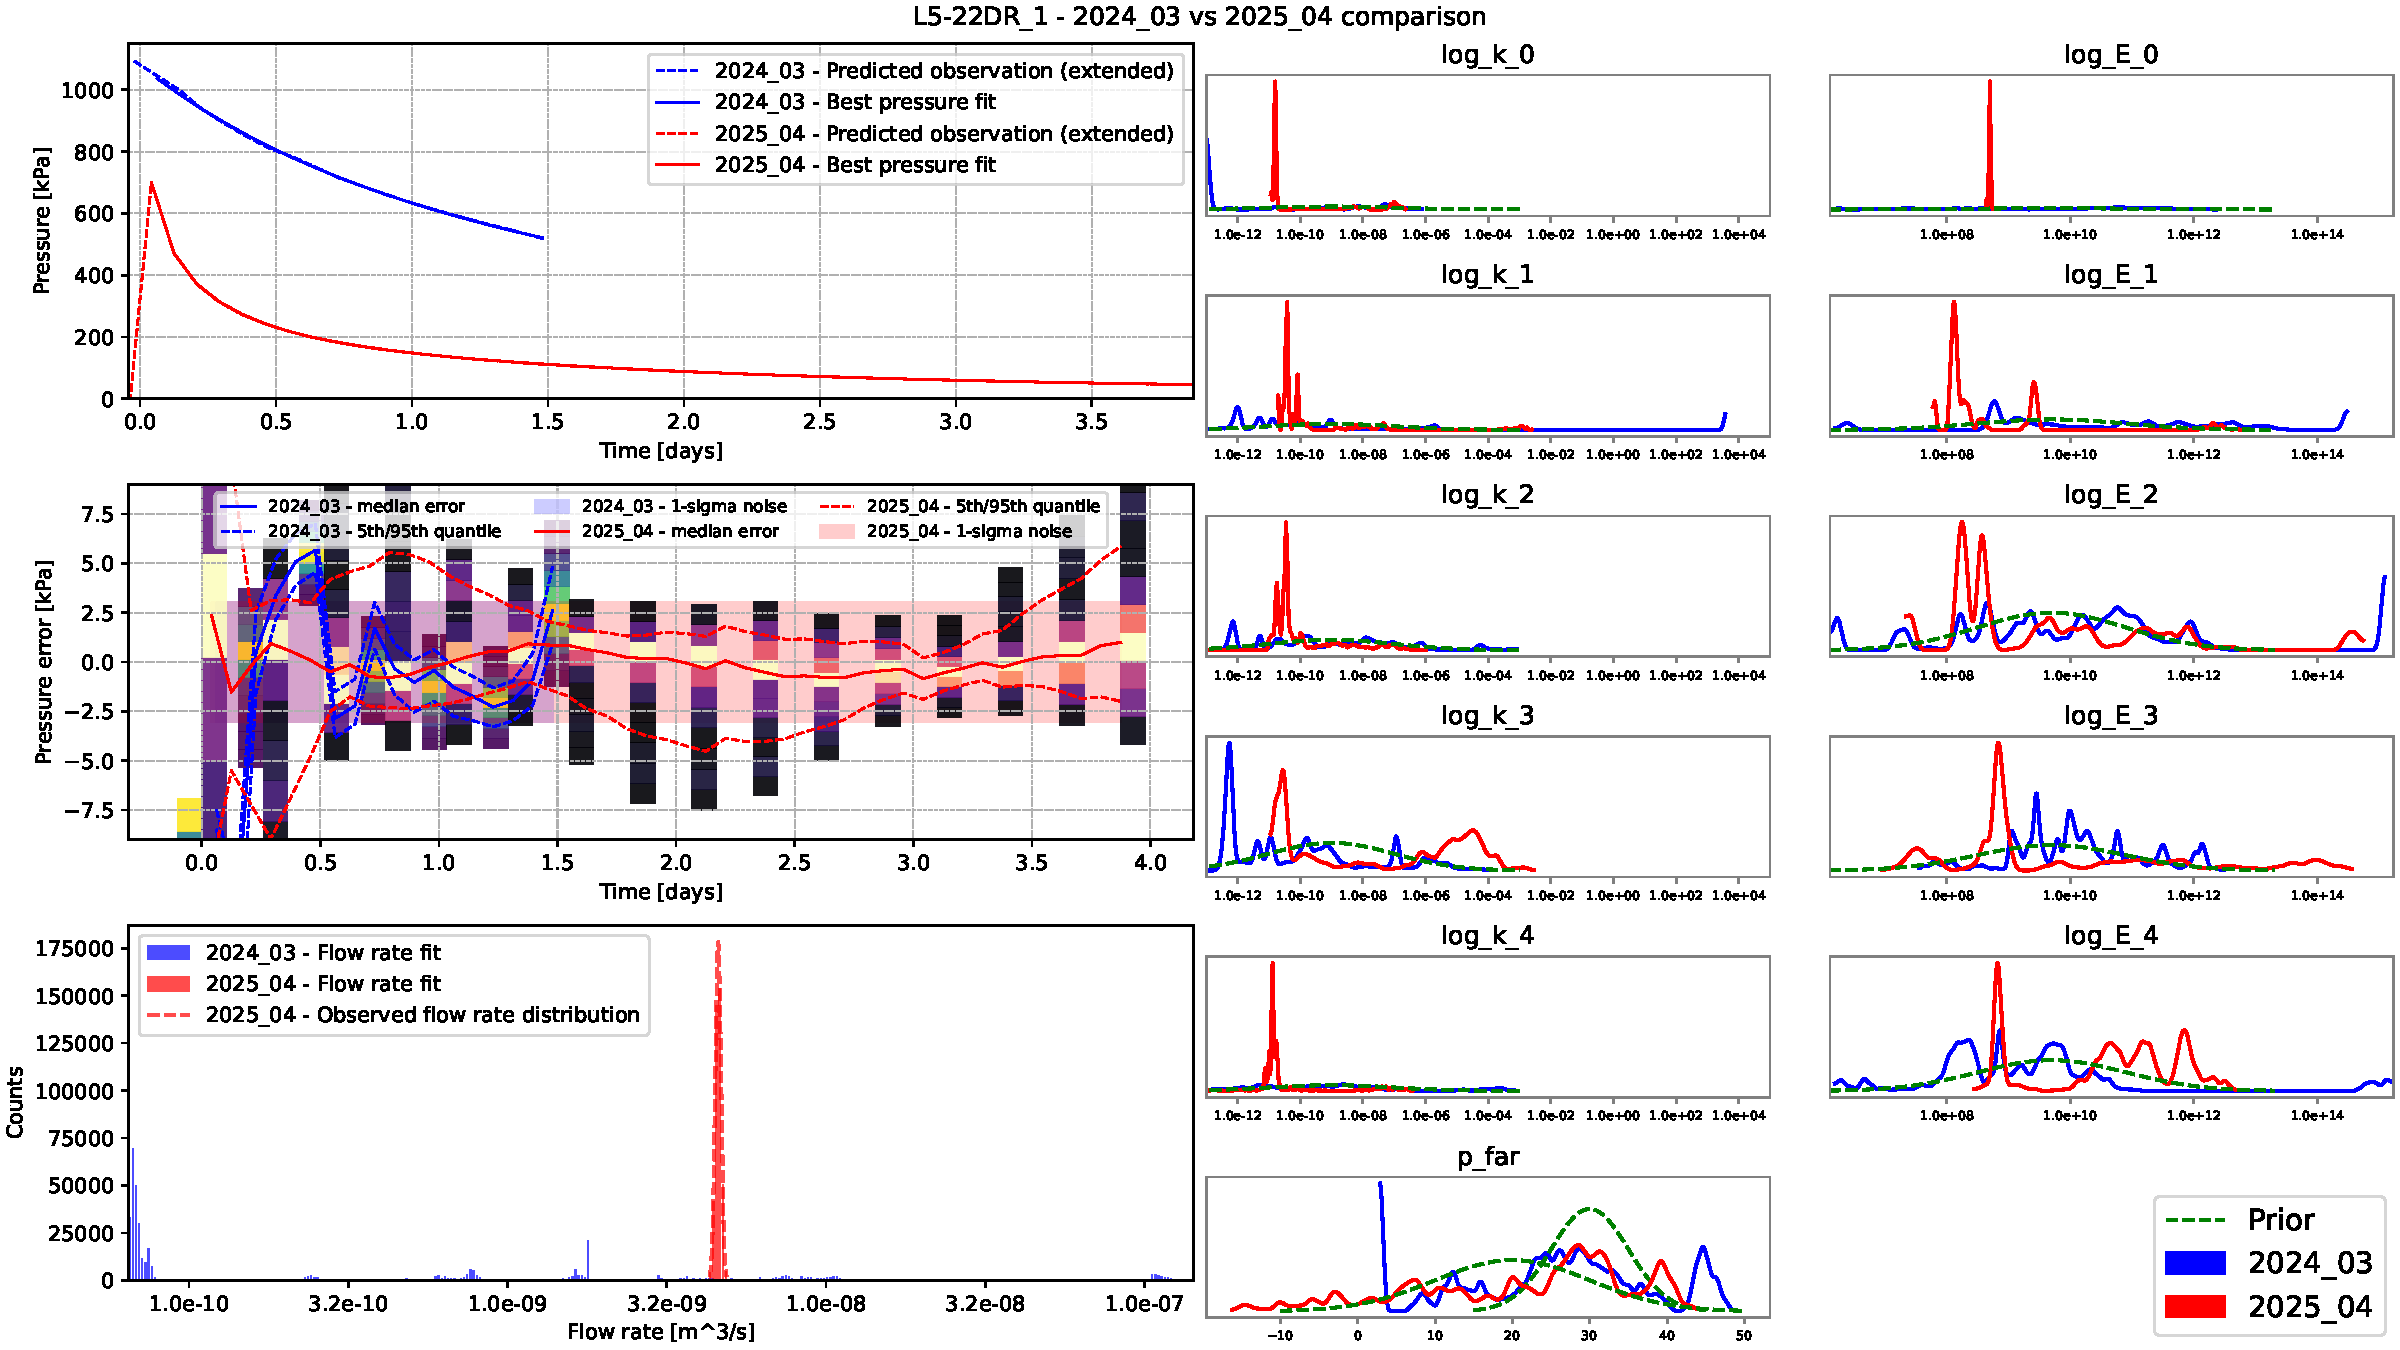
\includegraphics[width=0.75\textwidth]{PP_figs/22DR_1_compareplot.pdf}
    \end{center}
    \caption{Bayesian inversion summary for cell 22DR-1.}
    \label{fig:bayes_22DR_1}
\end{figure}
\begin{figure}
    \begin{center}
    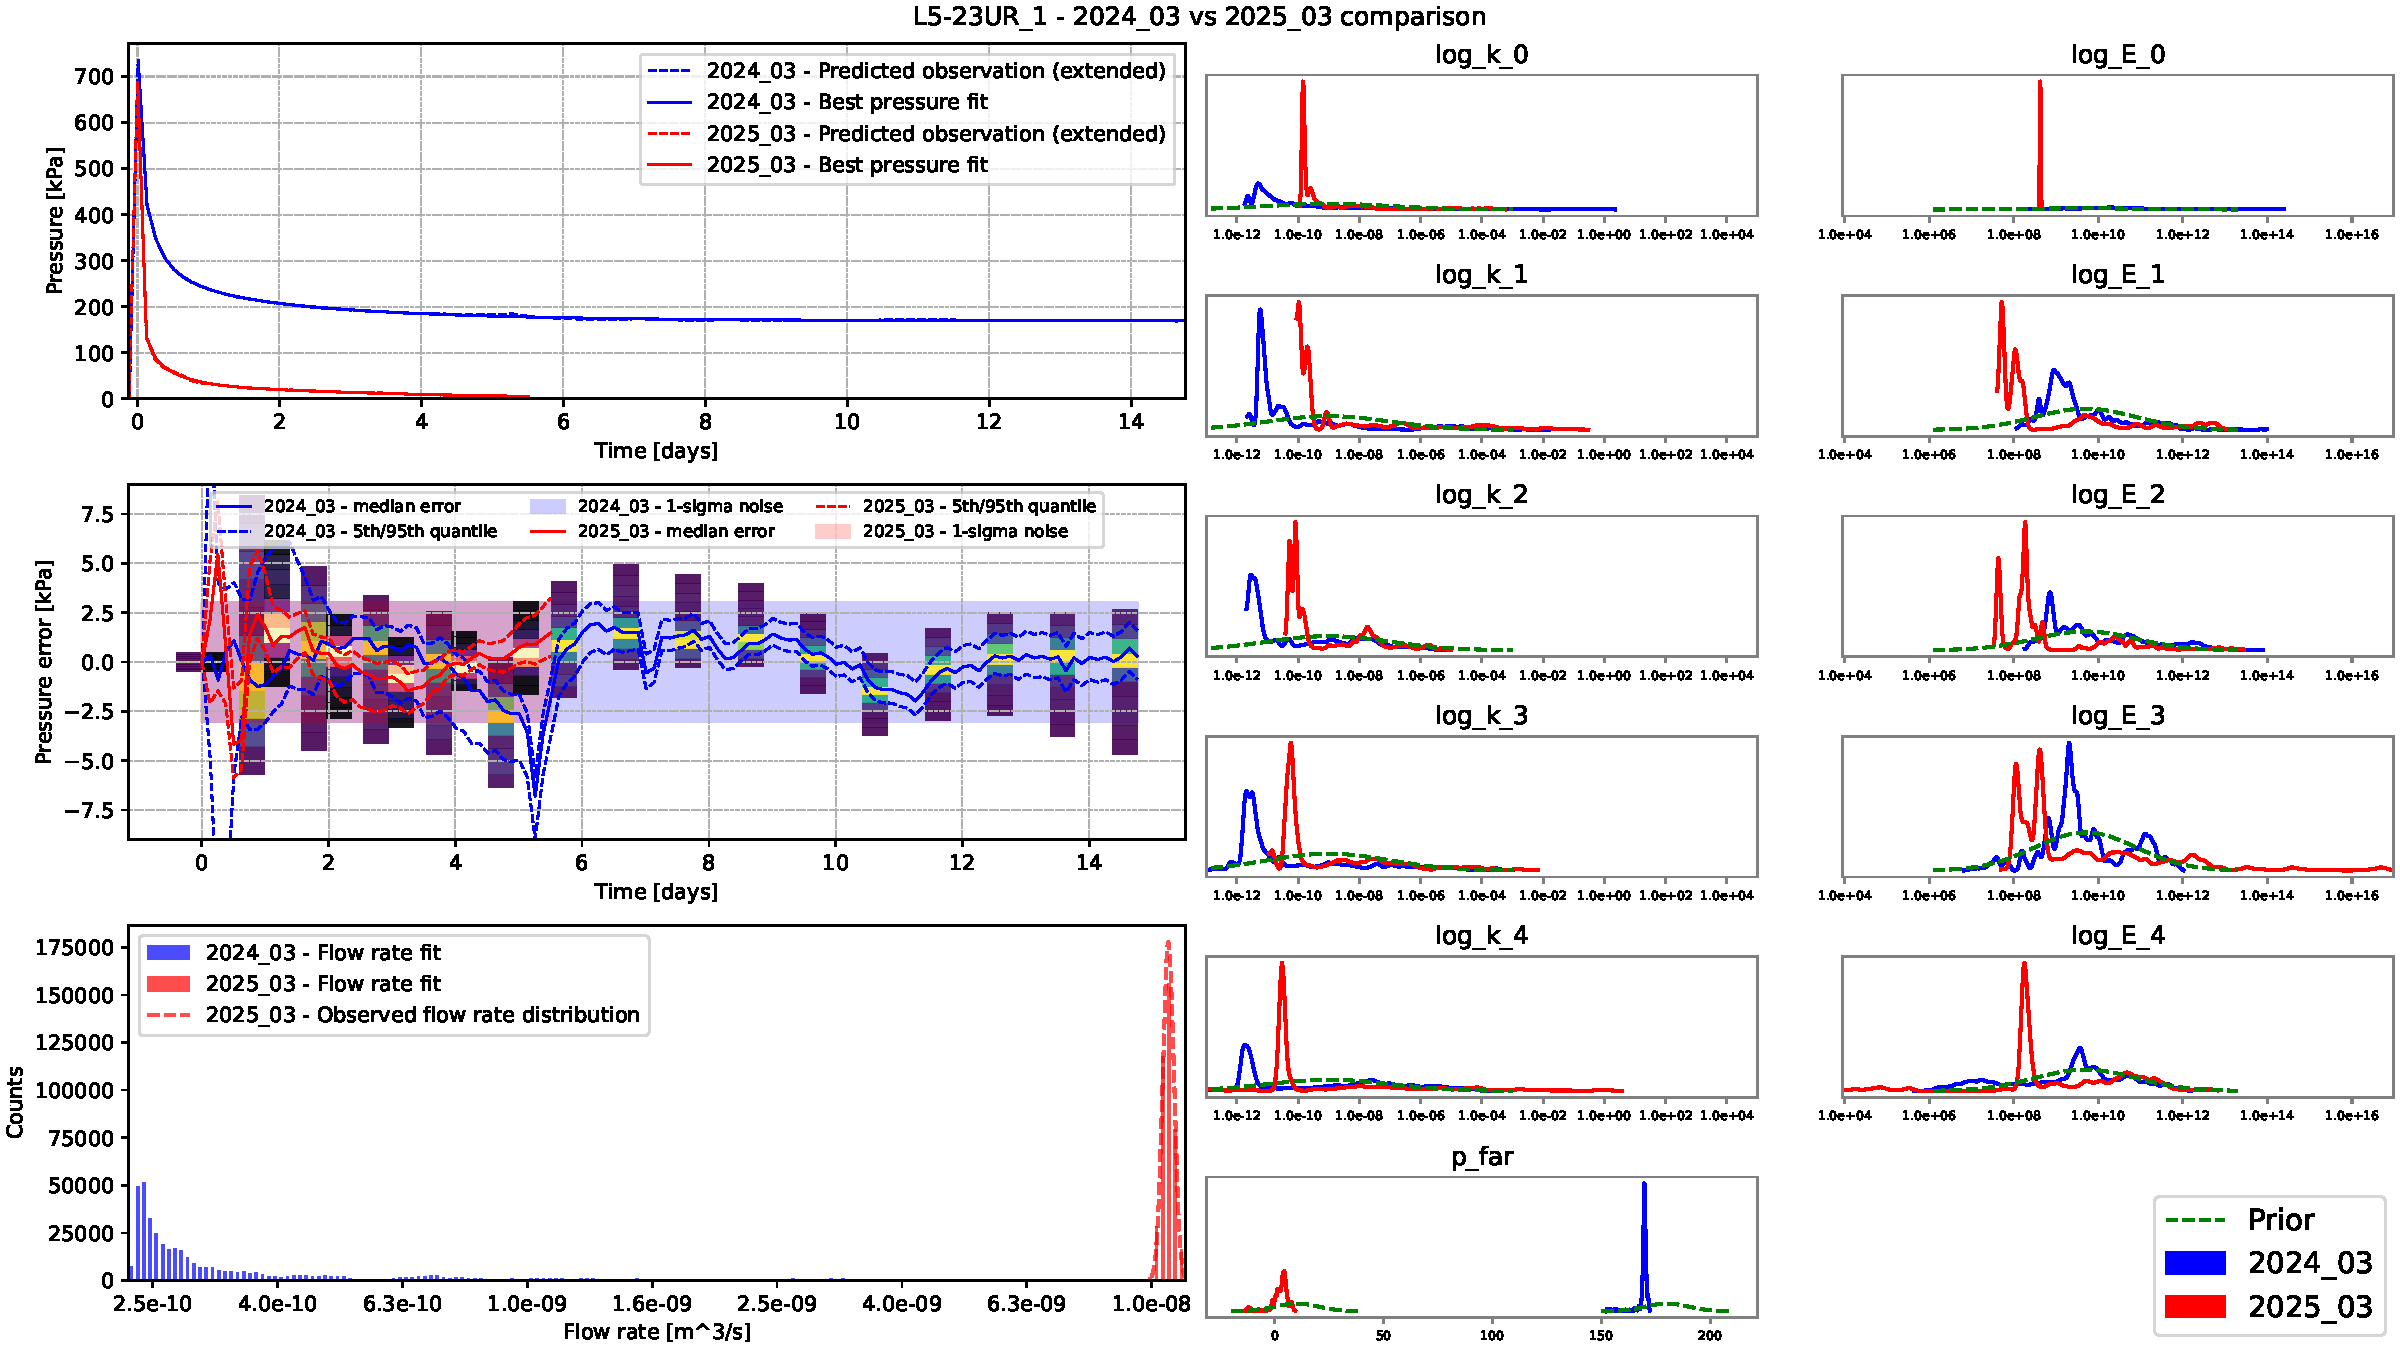
\includegraphics[width=0.75\textwidth]{PP_figs/23UR_1_compareplot.pdf}
    \end{center}
    \caption{Bayesian inversion summary for cell 23UR-1.}
    \label{fig:bayes_23UR_1}
\end{figure}
\FloatBarrier
\newpage
\begin{figure}
    \begin{center}
    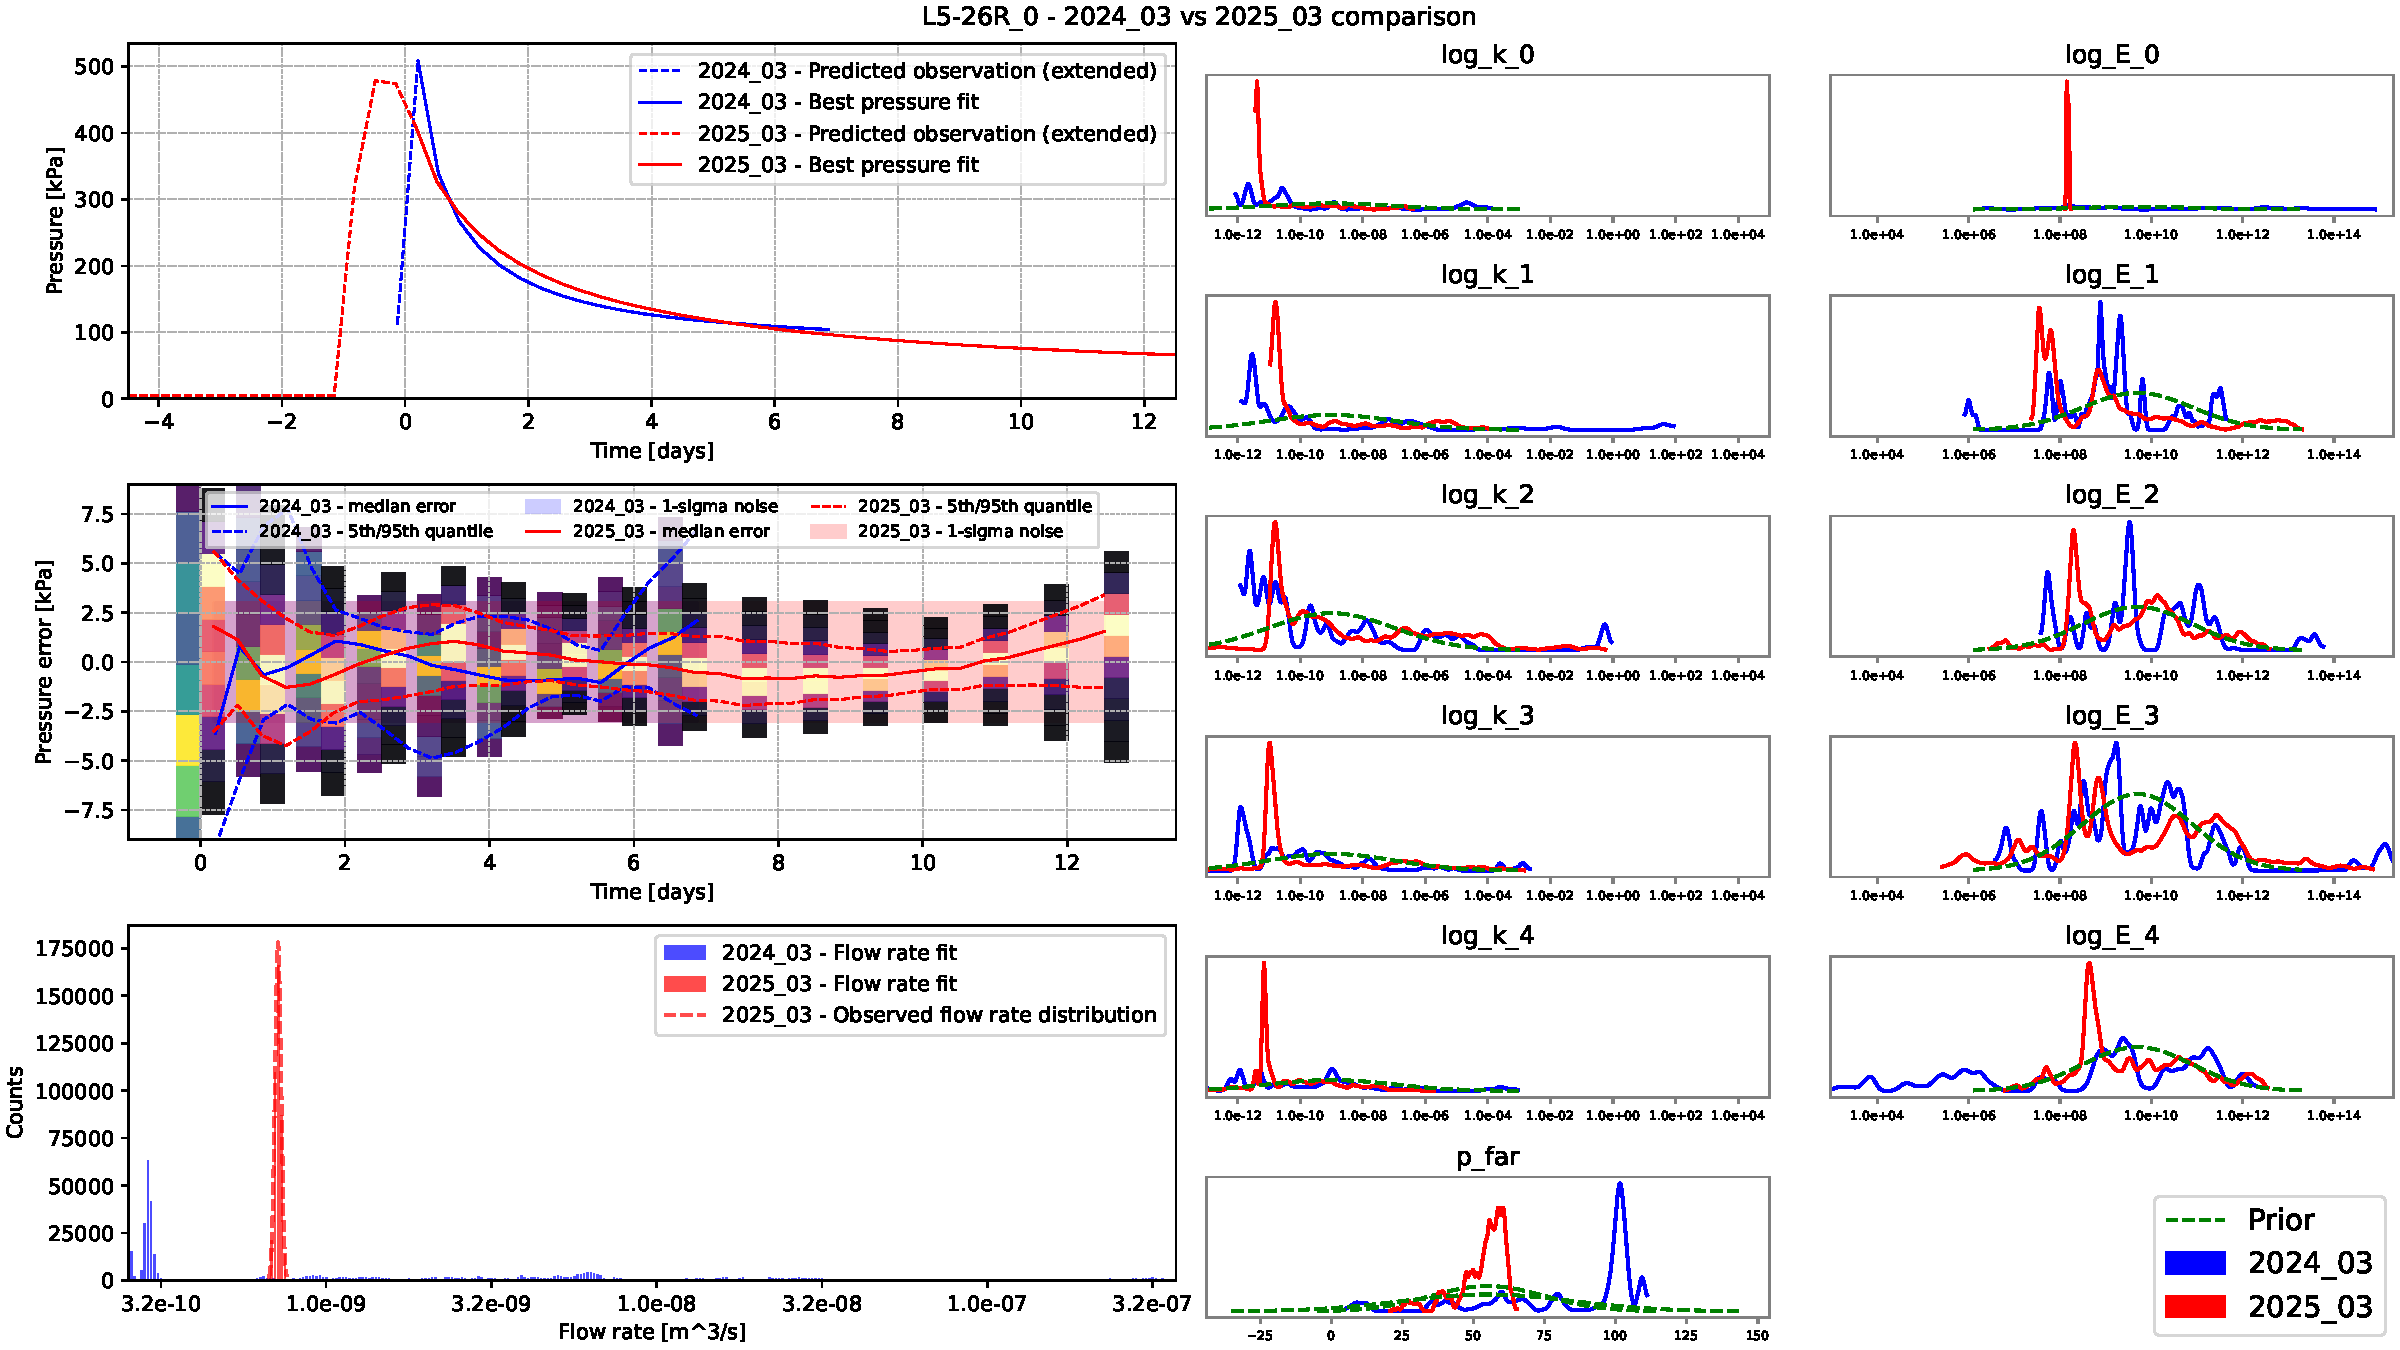
\includegraphics[width=0.75\textwidth]{PP_figs/26R_0_compareplot.pdf}
    \end{center}
    \caption{Bayesian inversion summary for cell 26R-0.}
    \label{fig:bayes_26R_0}
\end{figure}
\begin{figure}
    \begin{center}
    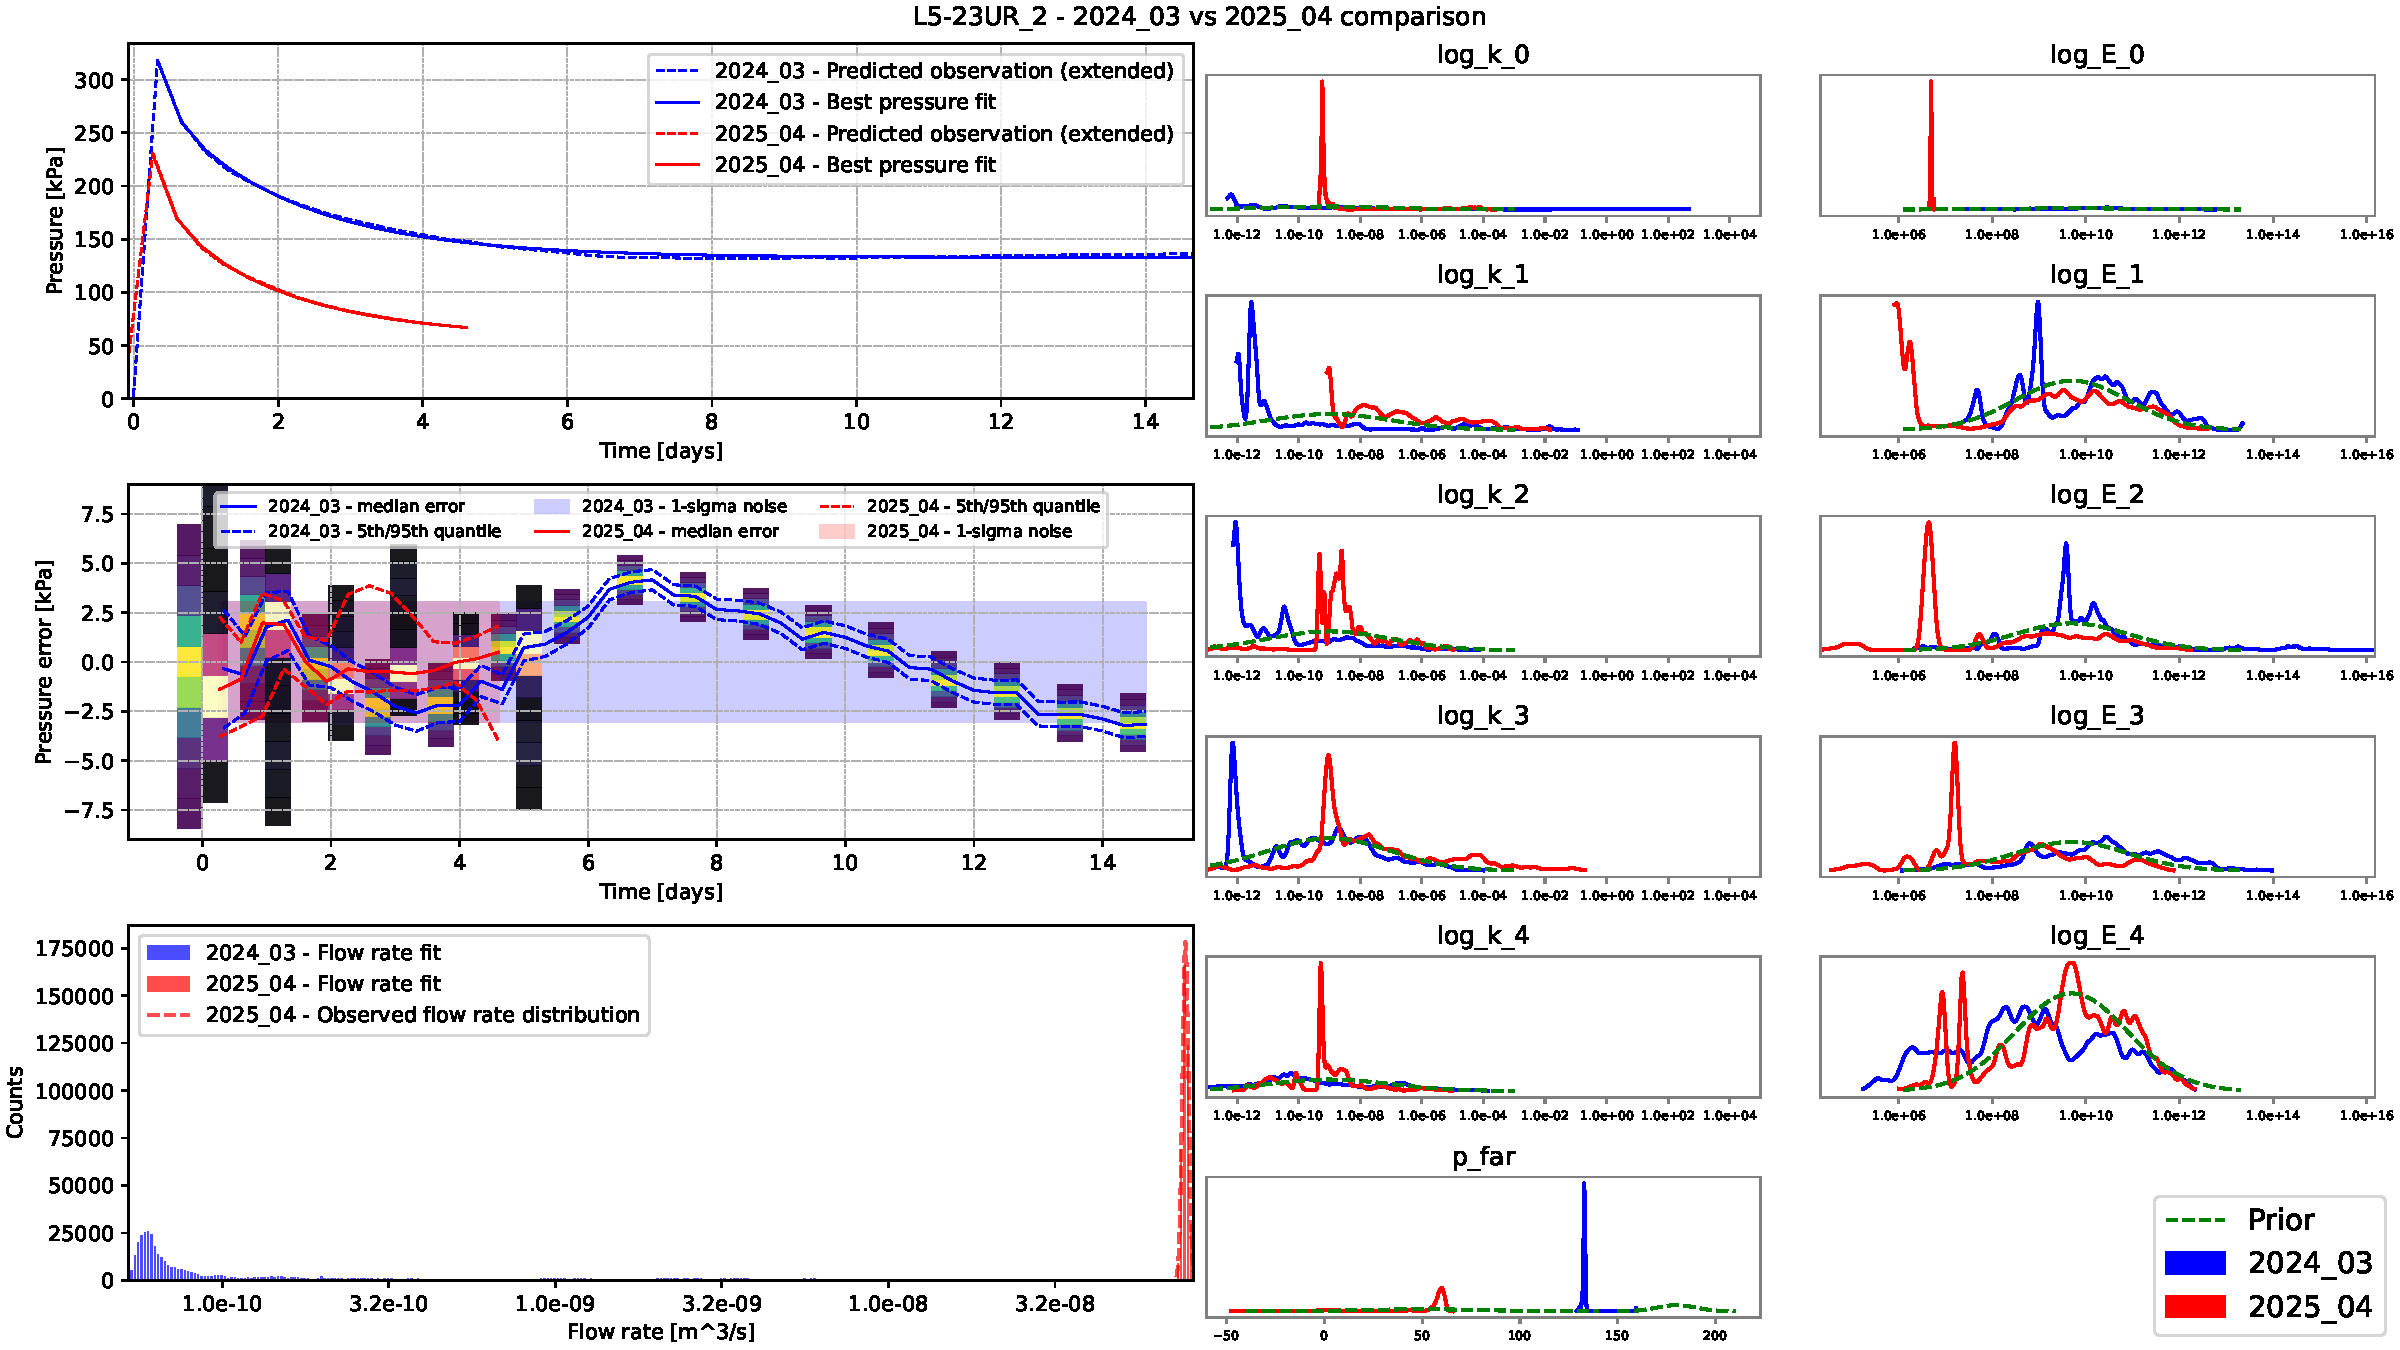
\includegraphics[width=0.75\textwidth]{PP_figs/23UR_2_compareplot.pdf}
    \end{center}
    \caption{Bayesian inversion summary for cell 23UR-2.}
    \label{fig:bayes_23UR_2}
\end{figure}
\begin{figure}
    \begin{center}
    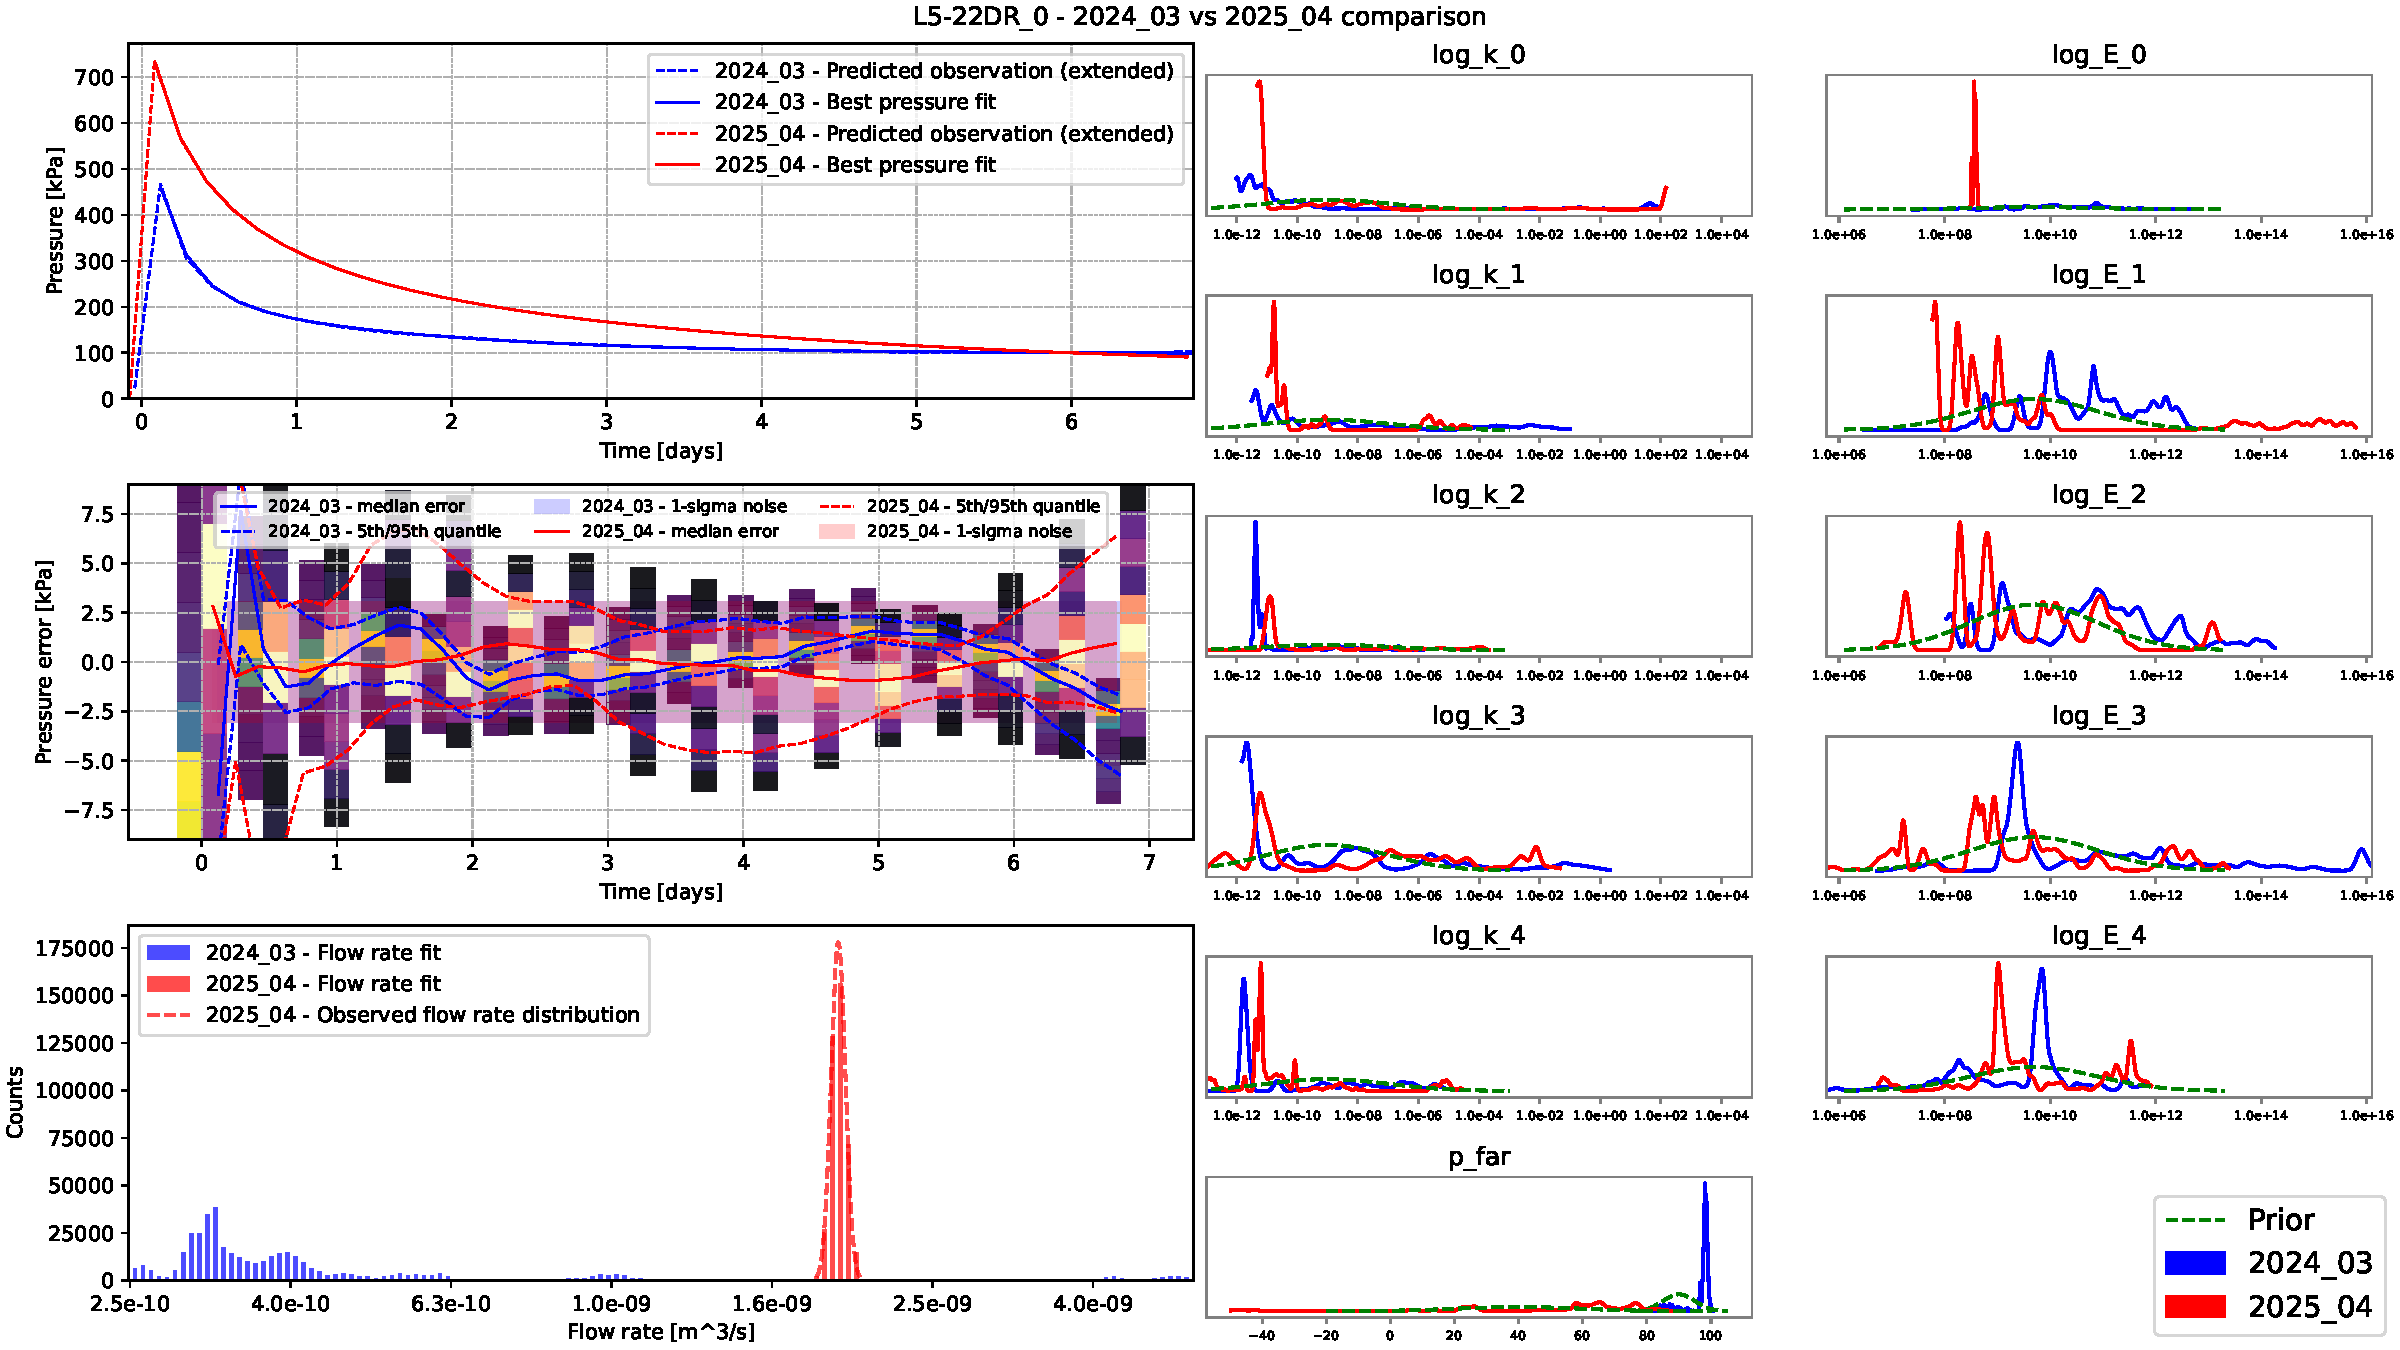
\includegraphics[width=0.75\textwidth]{PP_figs/22DR_0_compareplot.pdf}
    \end{center}
    \caption{Bayesian inversion summary for cell 22DR-0.}
    \label{fig:bayes_22DR_0}
\end{figure}
\FloatBarrier
\newpage

% Group 3 ======================================================================


\subsubsection{Low pressure south sensors}
The WPT comparison (Fig. \ref{fig:wpts_cases_13_18}) for the remaining south sensors
\region{24DR-2}, \region{24DR-1}, \region{24DR-0}, \region{37UR-1}, \region{37R-1}, and
\region{37UR-0} follows a common pattern: the post-excavation WPTs show a slower
pressure decay toward an elevated pressure level compared to the initial WPT. The
inversion plots (Fig. \ref{fig:bayes_24DR_2}) are not conclusive.

The sensor \region{23DR-2} declines after excavation to the lowest values of all measurements.
Within borehole \region{23DR}, the highest pressure is observed in \region{23DR-1}, about
60~kPa higher than in \region{23DR-2}. In August 2024, however, \region{23DR-1} rises and
\region{23DR-2} drops, effectively swapping their ranking. These abrupt changes remain
unexplained.

The sensor \region{37UR-1} returns immediately to near-zero pressure after the initial
WPT and shows almost no response to excavation. The decay after the 2025 WPT is
slightly slower. The equilibrium pressure slowly increases in the second half of
2025, followed by a similar pattern in \region{37R-1}.



\begin{figure}[t]
    \begin{center}
    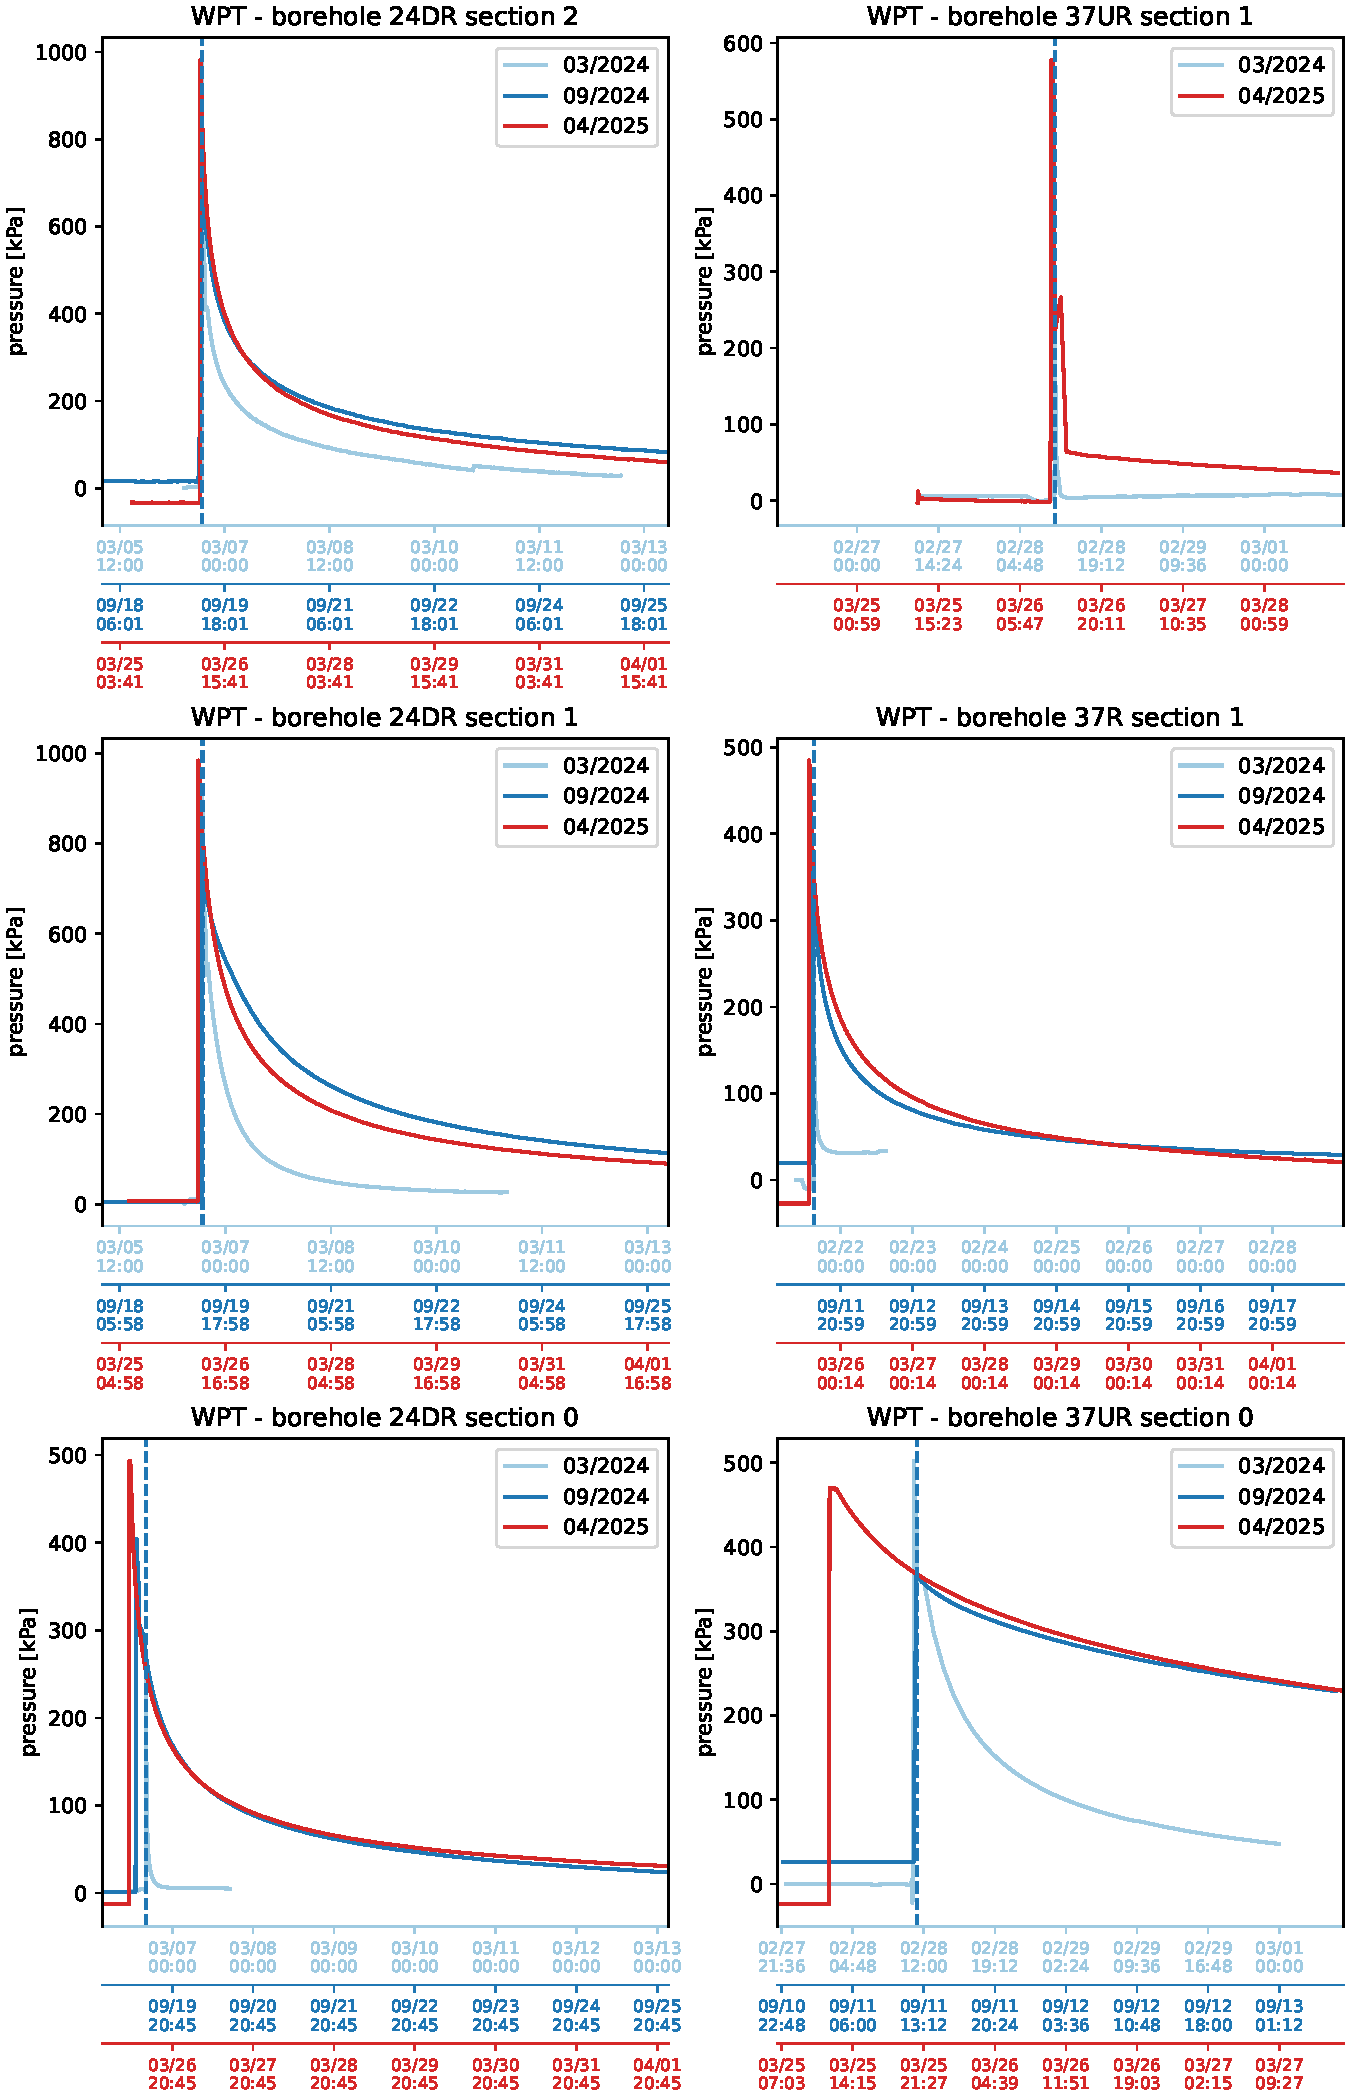
\includegraphics[width=0.9\textwidth]{PP_figs/wpt_grid_03.pdf}
    \end{center}
    \caption{Stitched water pressure test plots 03.}
    \label{fig:wpts_cases_13_18}
\end{figure}
\FloatBarrier
\newpage
\begin{figure}
    \begin{center}
    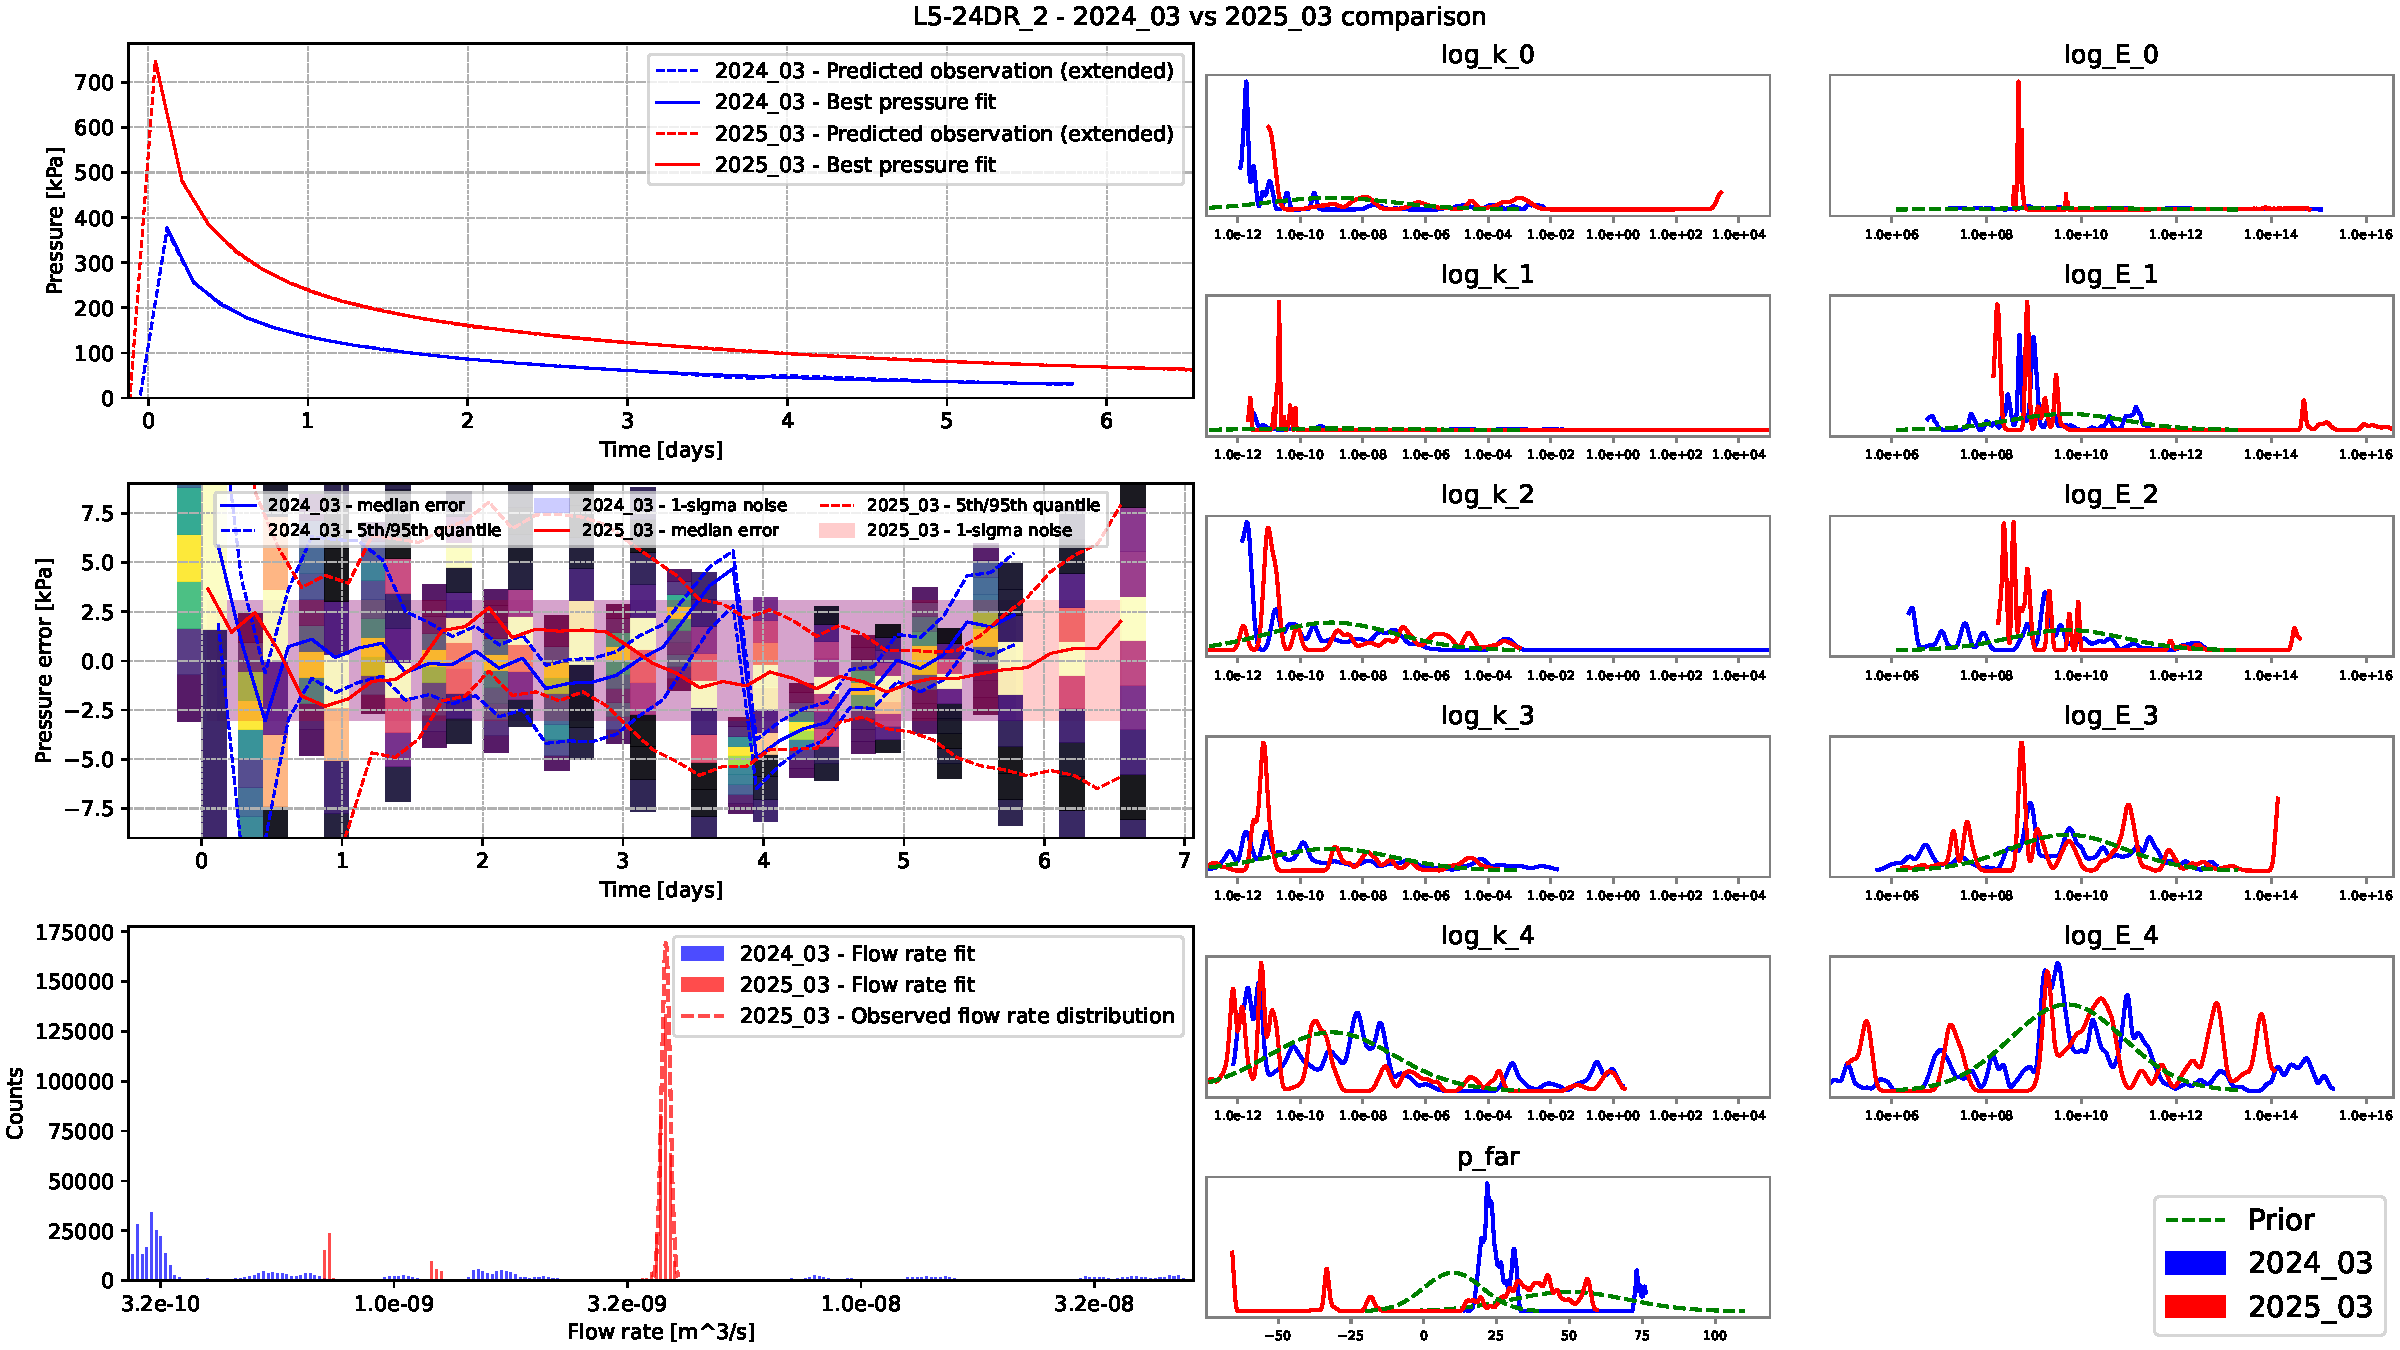
\includegraphics[width=0.75\textwidth]{PP_figs/24DR_2_compareplot.pdf}
    \end{center}
    \caption{Bayesian inversion summary for cell 24DR-2.}
    \label{fig:bayes_24DR_2}
\end{figure}
\begin{figure}
    \begin{center}
    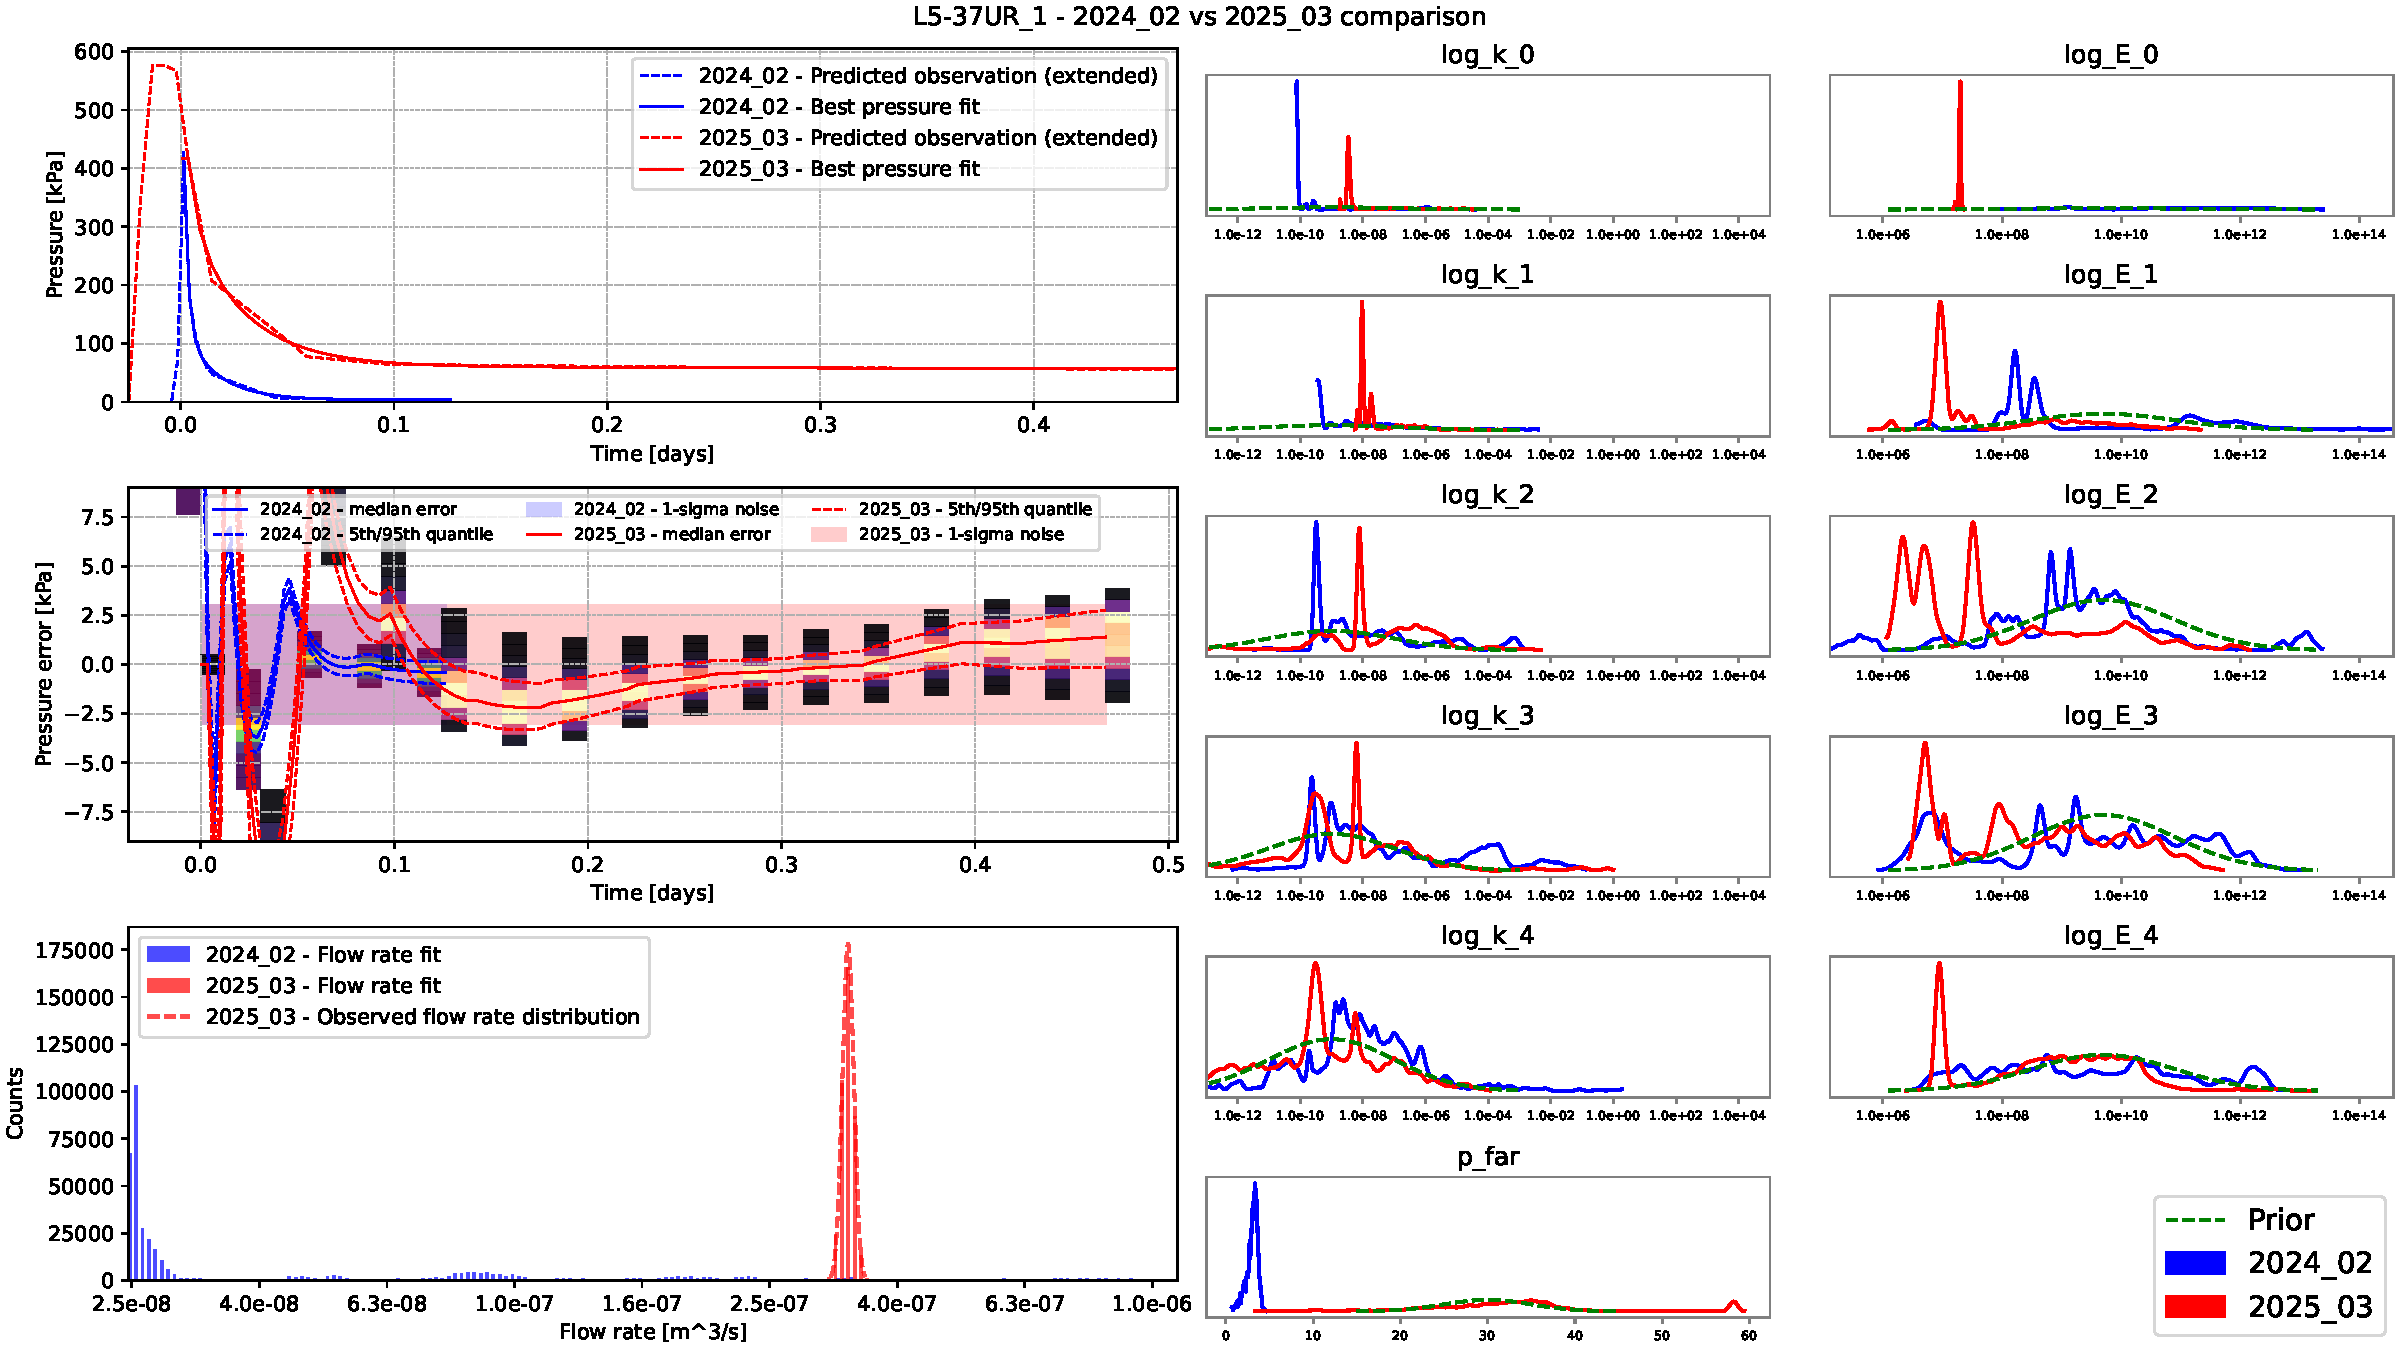
\includegraphics[width=0.75\textwidth]{PP_figs/37UR_1_compareplot.pdf}
    \end{center}
    \caption{Bayesian inversion summary for cell 37UR-1.}
    \label{fig:bayes_37UR_1}
\end{figure}
\begin{figure}
    \begin{center}
    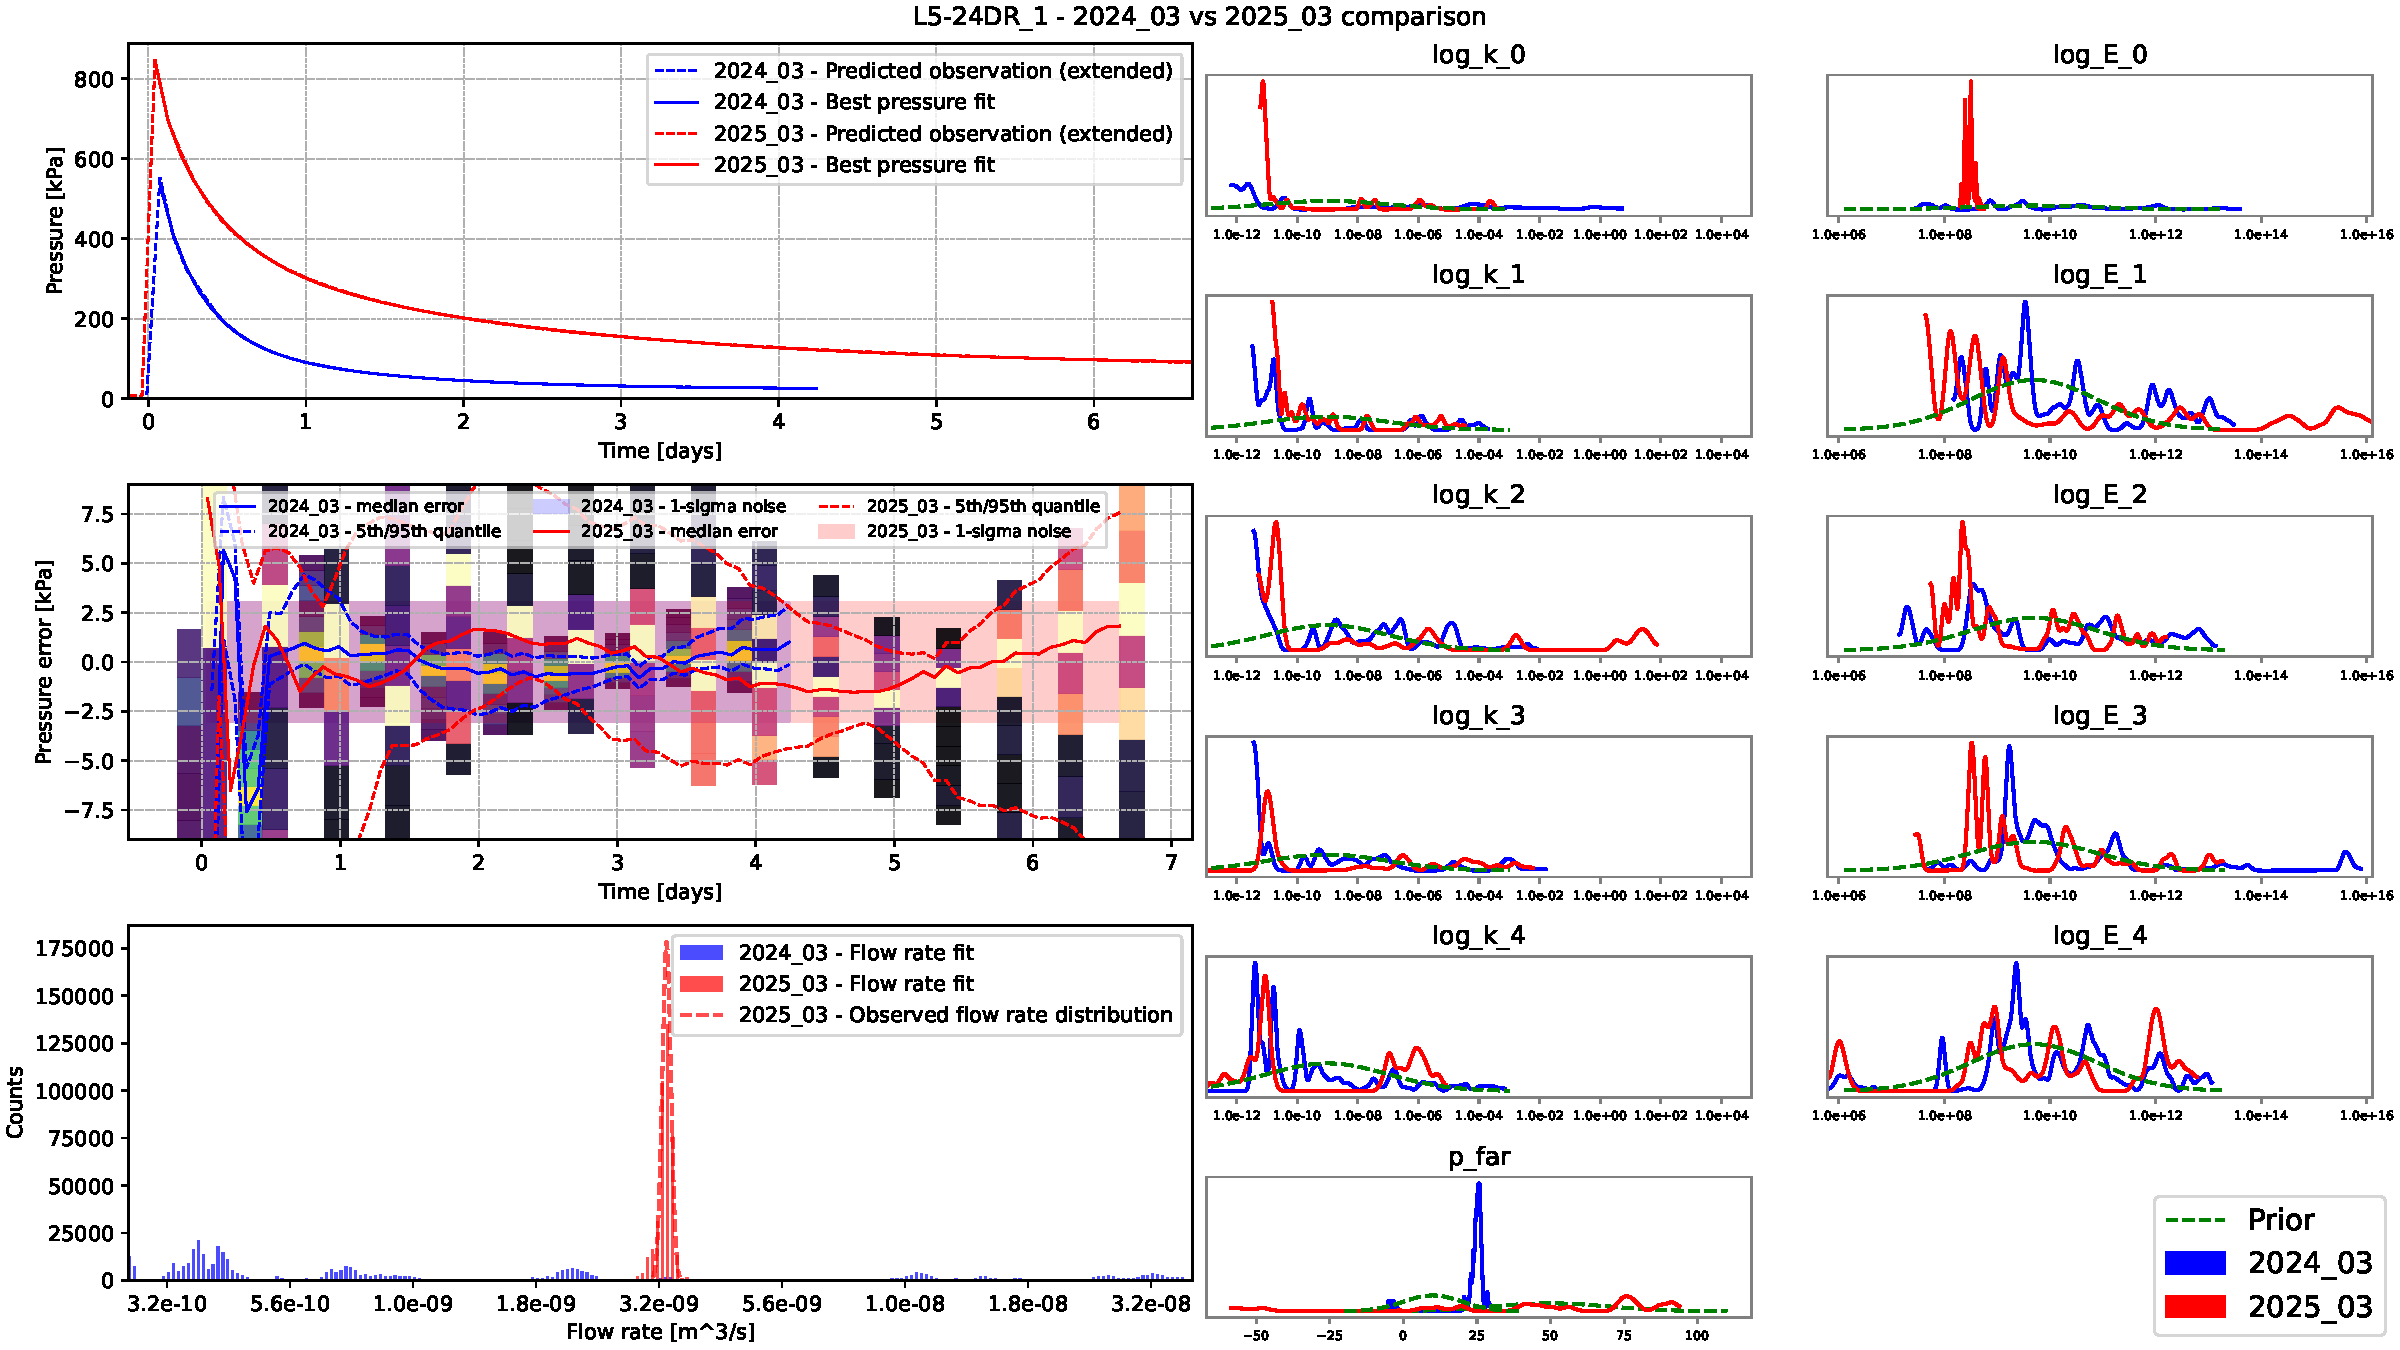
\includegraphics[width=0.75\textwidth]{PP_figs/24DR_1_compareplot.pdf}
    \end{center}
    \caption{Bayesian inversion summary for cell 24DR-1.}
    \label{fig:bayes_24DR_1}
\end{figure}
\FloatBarrier
\newpage
\begin{figure}
    \begin{center}
    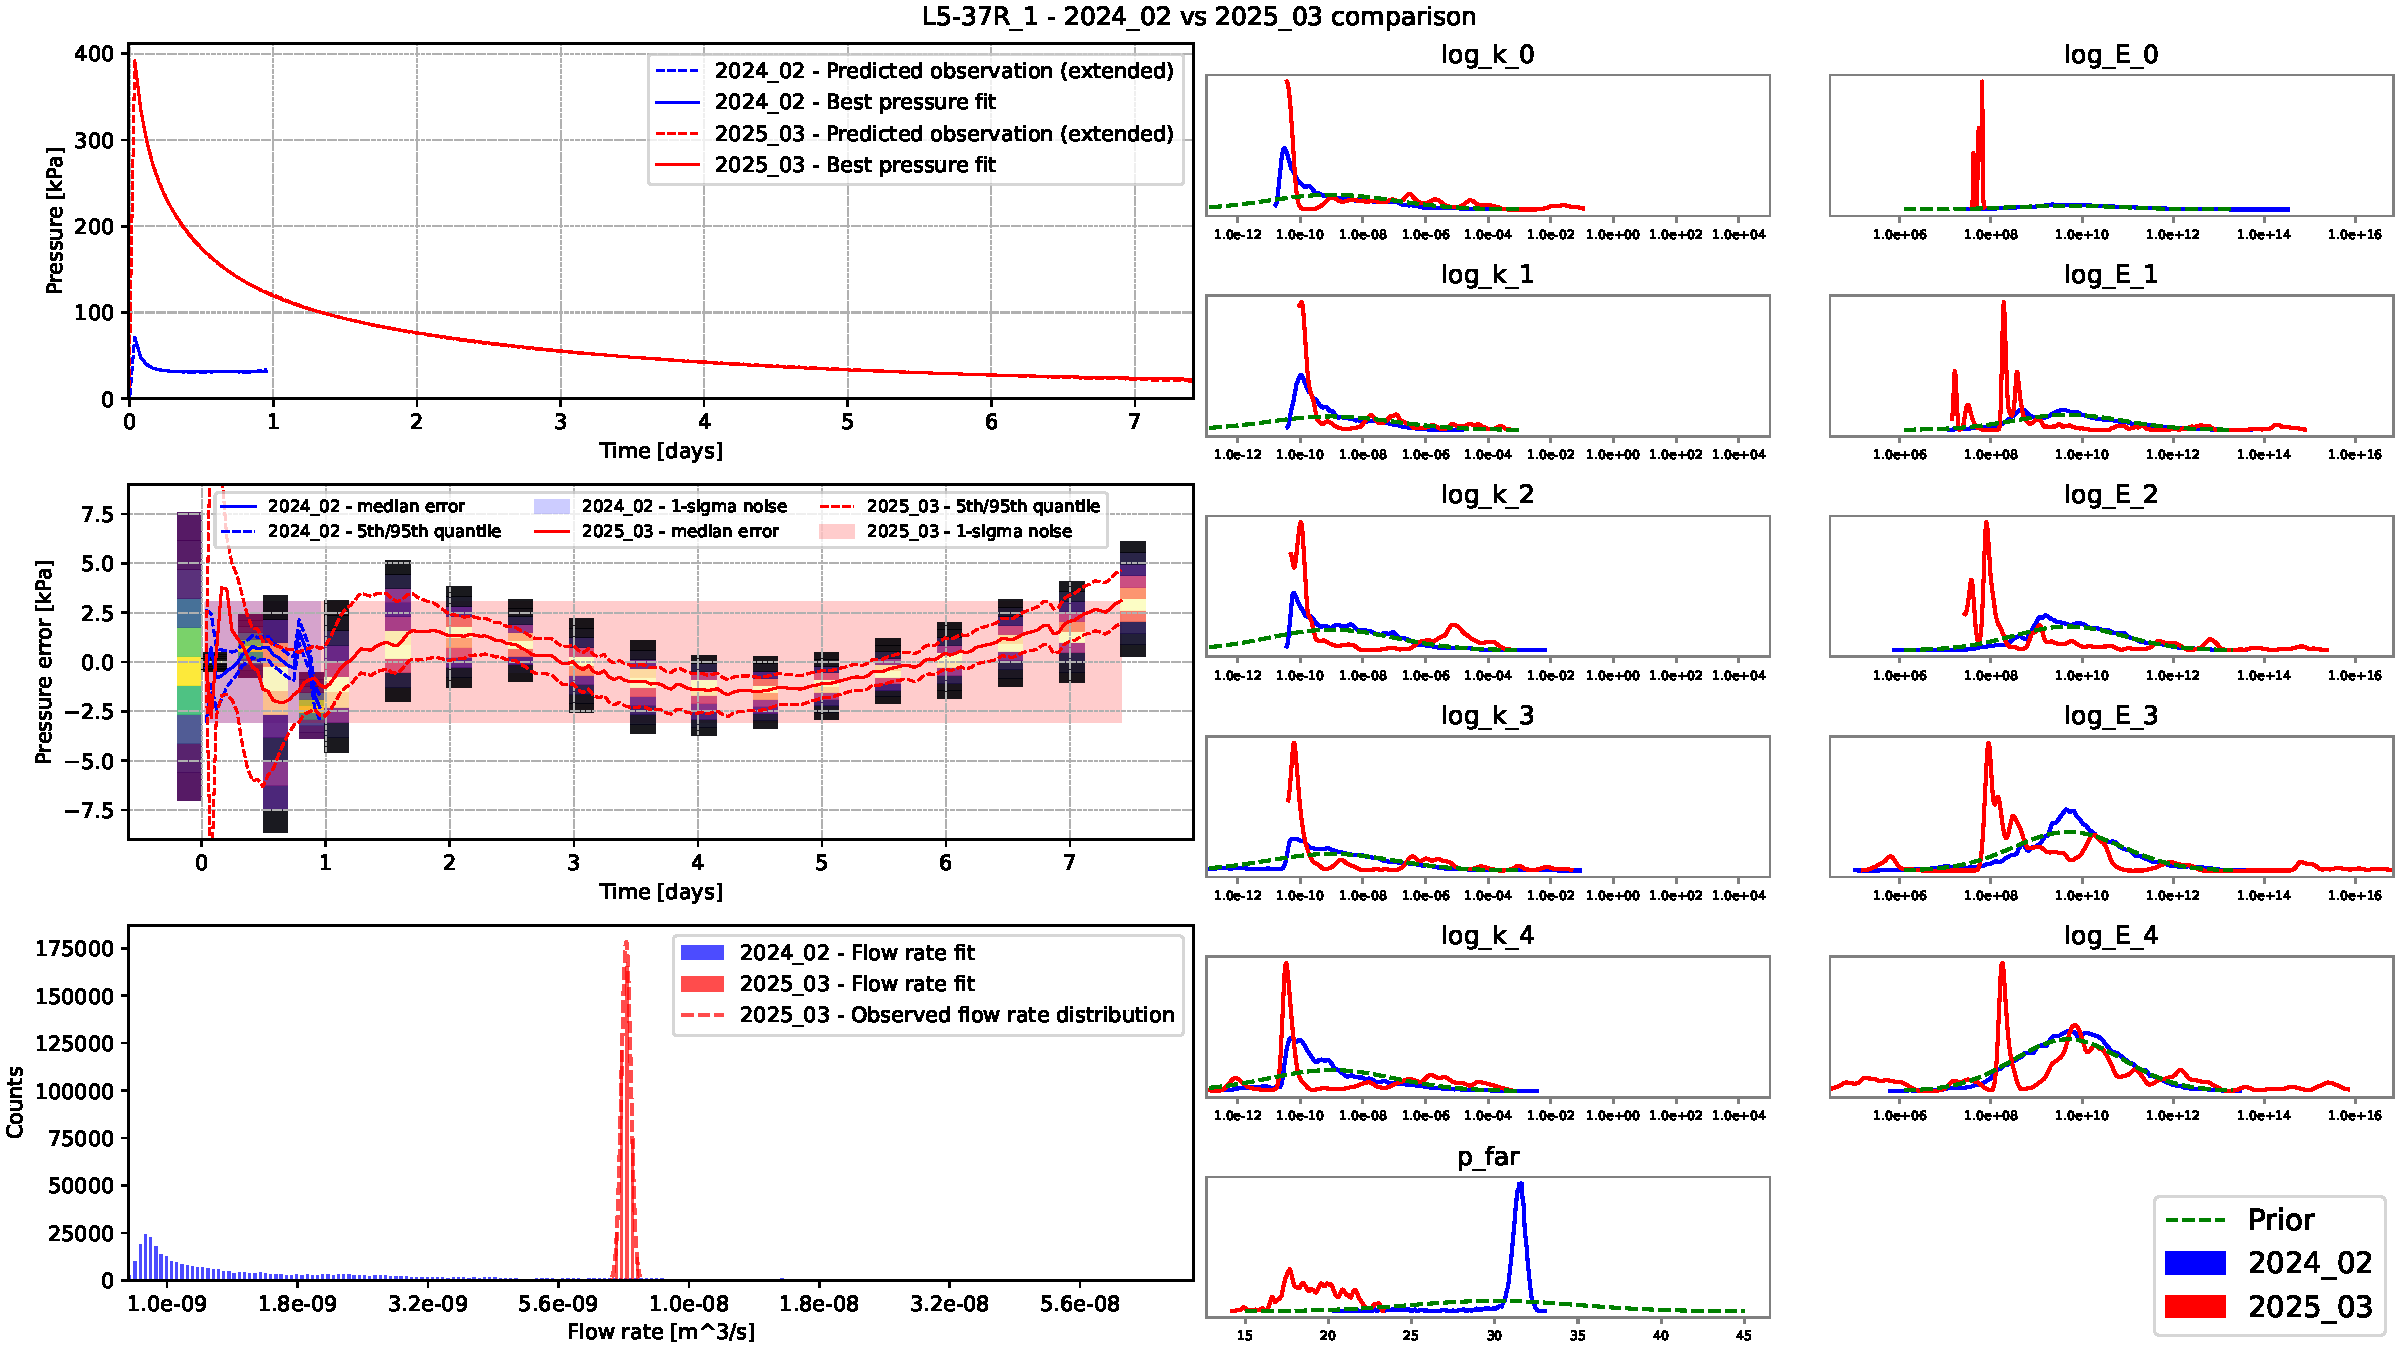
\includegraphics[width=0.75\textwidth]{PP_figs/37R_1_compareplot.pdf}
    \end{center}
    \caption{Bayesian inversion summary for cell 37R-1.}
    \label{fig:bayes_37R_1}
\end{figure}
\begin{figure}
    \begin{center}
    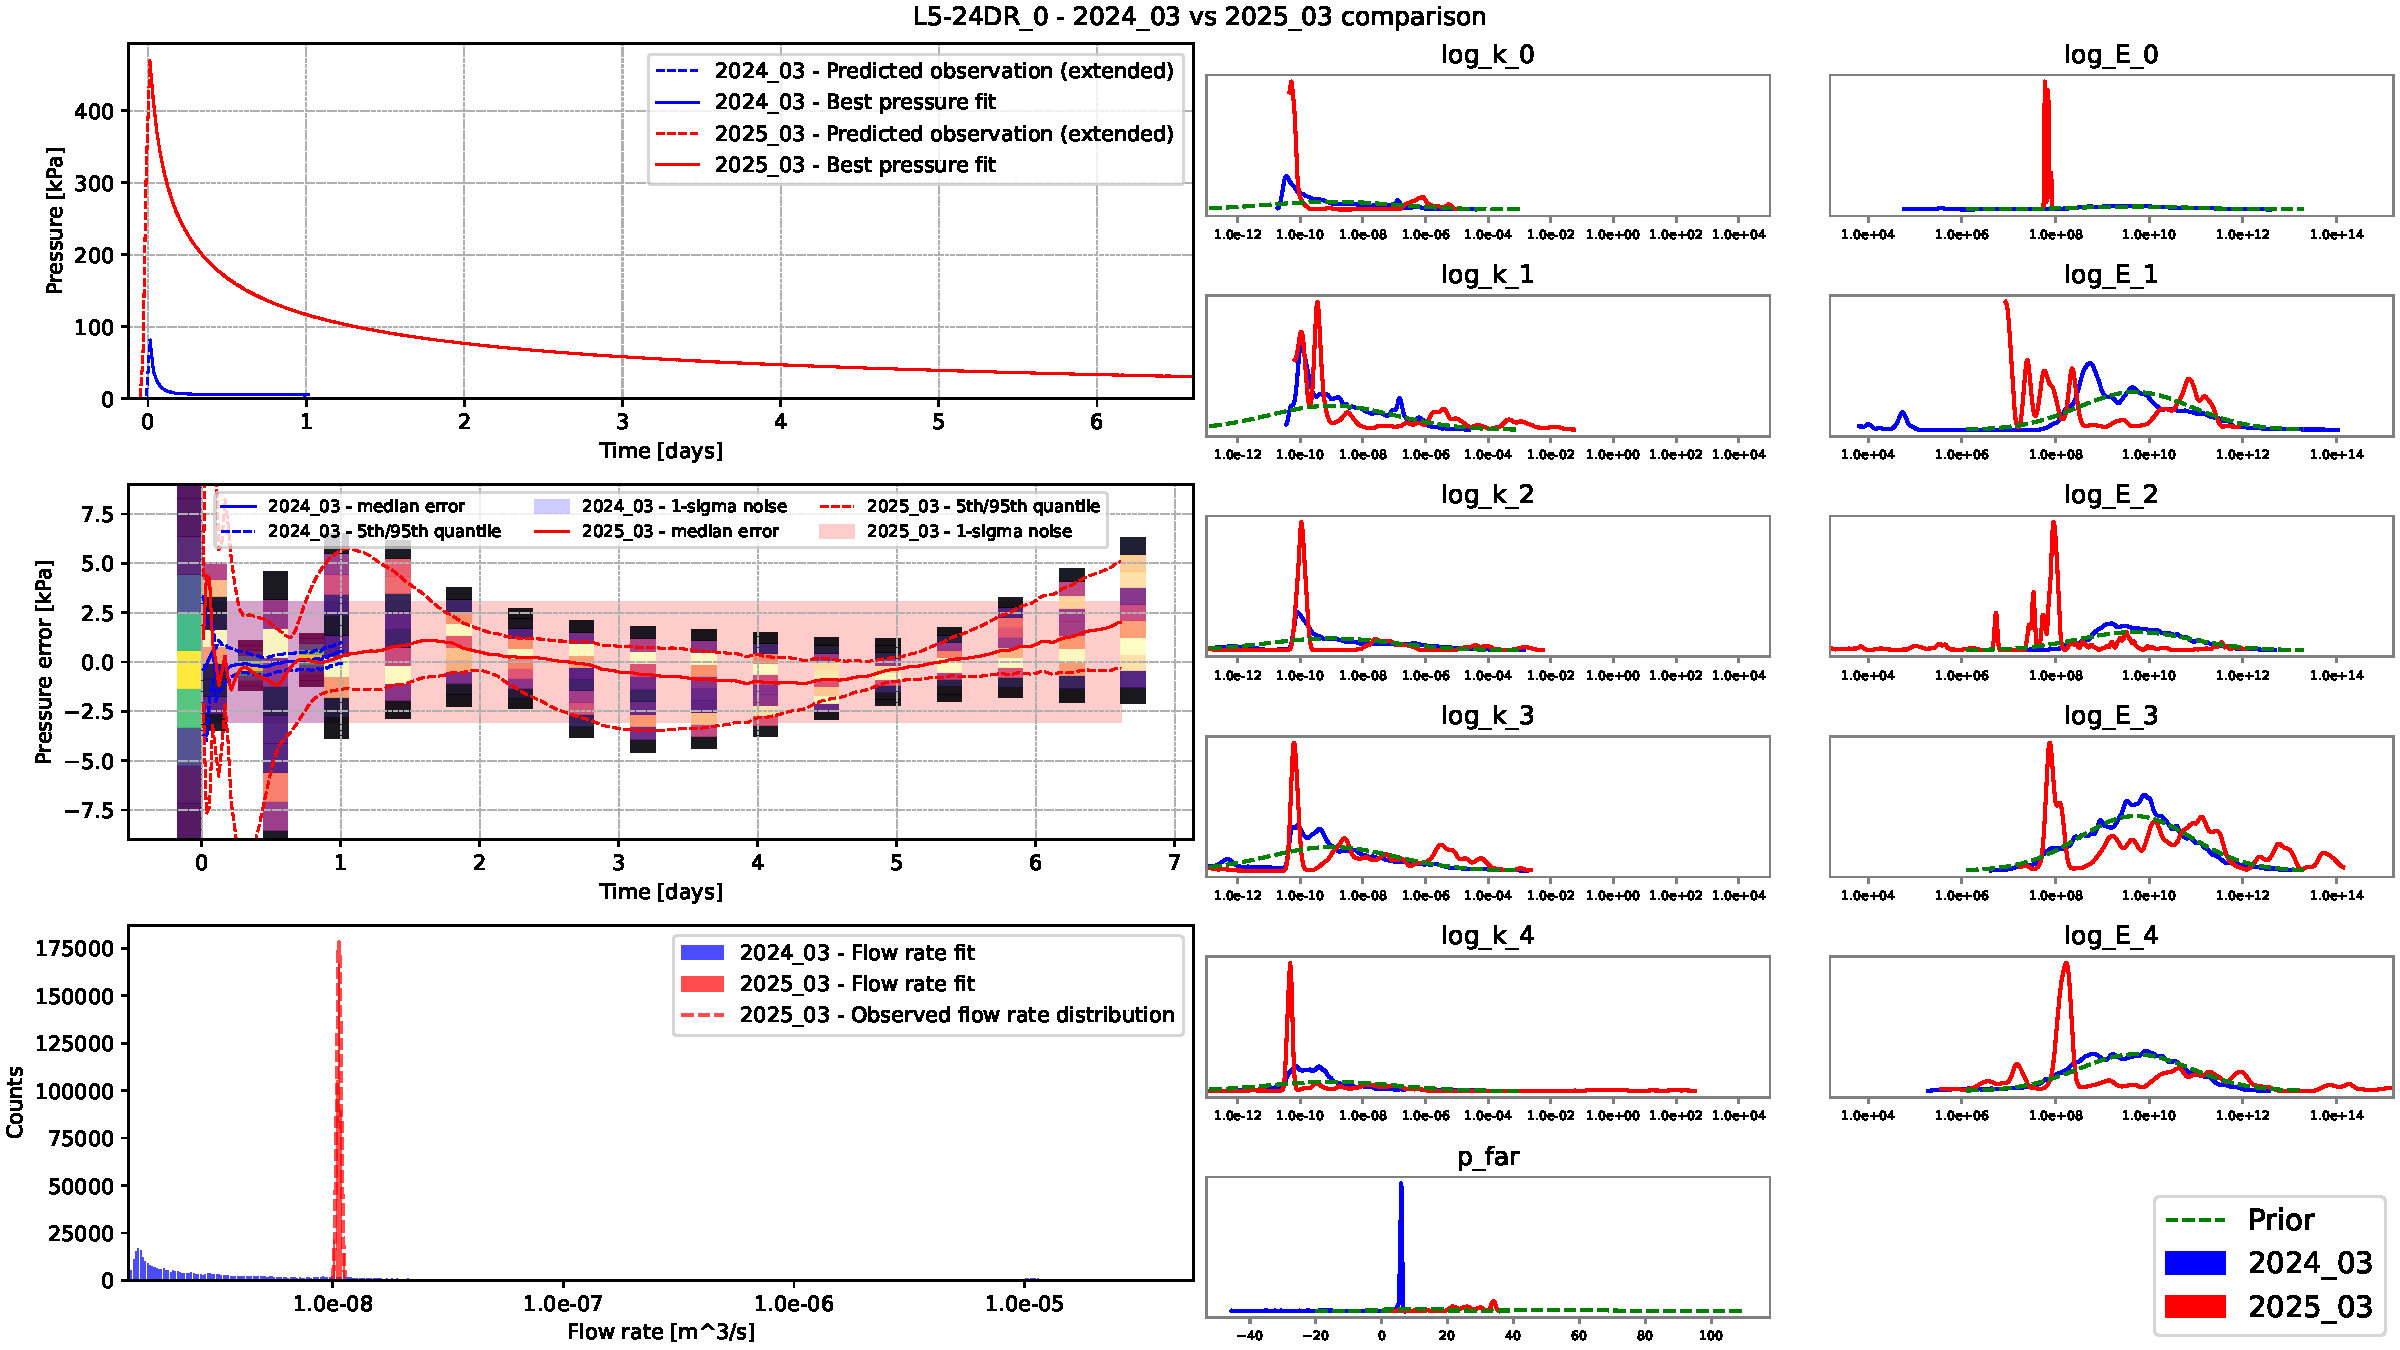
\includegraphics[width=0.75\textwidth]{PP_figs/24DR_0_compareplot.pdf}
    \end{center}
    \caption{Bayesian inversion summary for cell 24DR-0.}
    \label{fig:bayes_24DR_0}
\end{figure}
\begin{figure}
    \begin{center}
    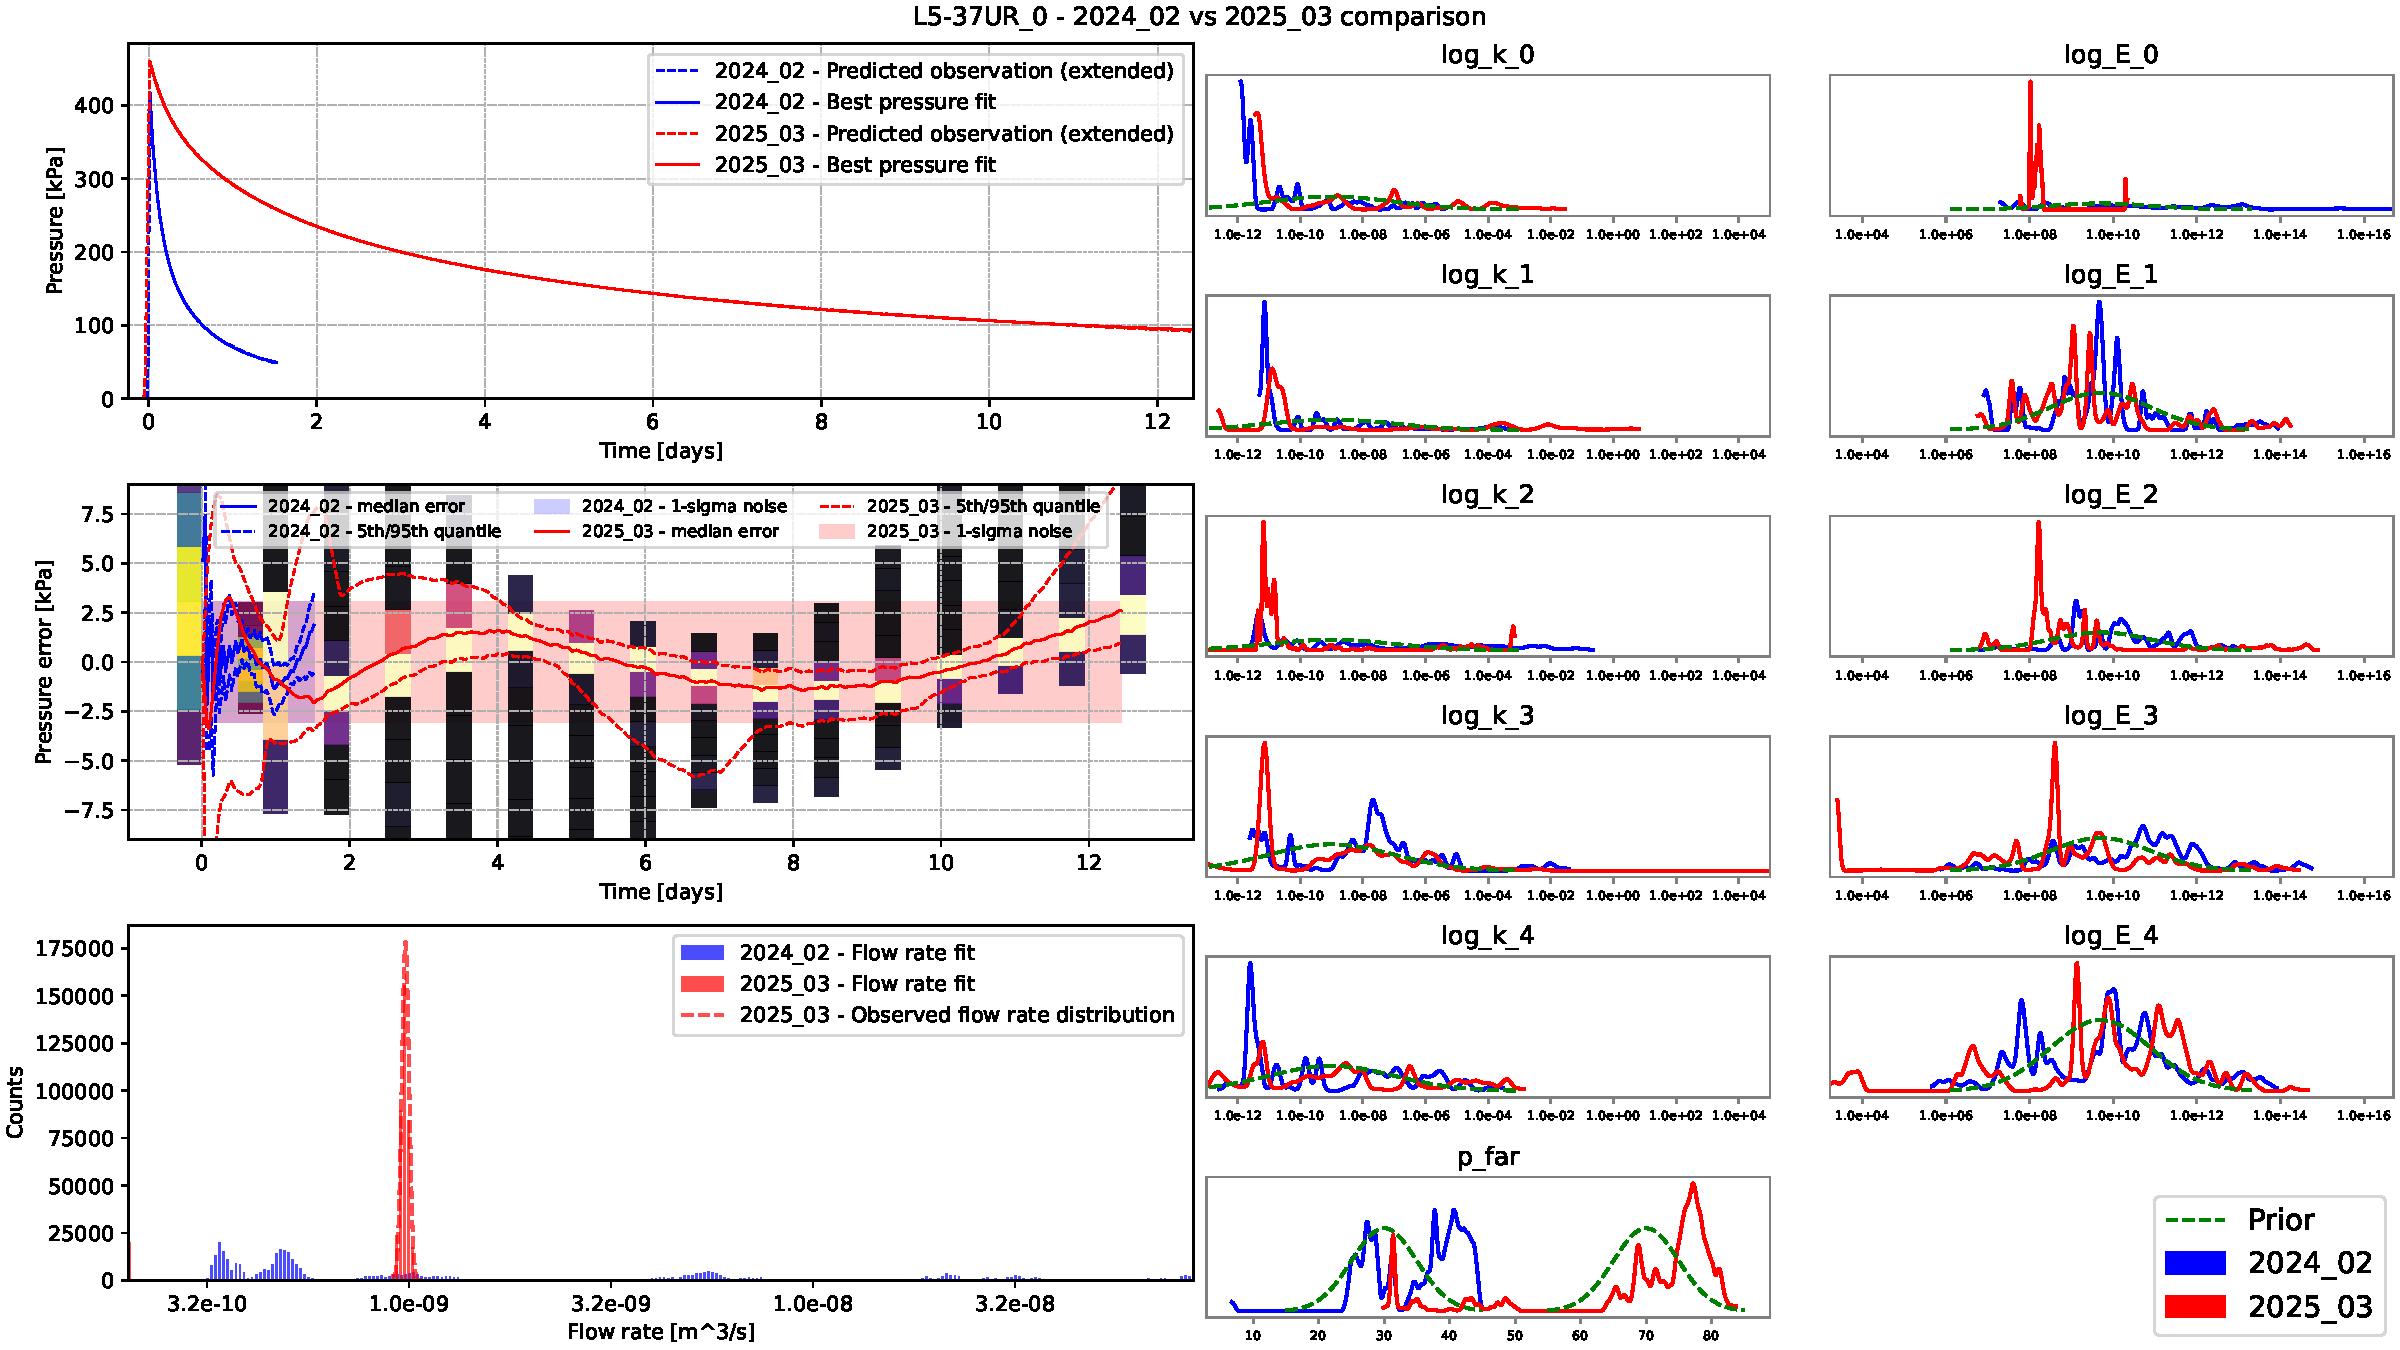
\includegraphics[width=0.75\textwidth]{PP_figs/37UR_0_compareplot.pdf}
    \end{center}
    \caption{Bayesian inversion summary for cell 37UR-0.}
    \label{fig:bayes_37UR_0}
\end{figure}
\FloatBarrier
\newpage
% Group 4 ======================================================================
\subsubsection{North boreholes sensors}

The rock mass around the north chamber was expected to be even more heterogeneous
than around the south chamber, possibly influenced by a nearby highly conductive
fault zone. All sensors return to the baseline pressure within one day after the
WPTs (Fig. \ref{fig:wpts_cases_19_24}). The water fluxes measured during the
2025 WPTs are all above $10^{-1} \munit{ml/s}$, with the exception of \region{50UL-0} and
\region{49UL-2}, where the fluxes are about $10^{-2} \munit{ml/s}$; these values are
comparable to the highest fluxes measured in the south cells
(Fig. \ref{fig:flow_summary}).

Three WPTs were performed in borehole \region{50UL}. The first one was followed by
an immediate return to near-zero pressure, and the second one shows an exponential
decline. The third WPT exhibits an unusual response on sensors \region{50UL-1} and
\region{50UL-0}. The signal profiles are very similar, with a higher and sharper
reading on \region{50UL-1} and a smoother response on \region{50UL-0}.

The response to the excavation is very mild. Positive peaks are observed only on
\region{50UL-1} and \region{50UL-0} during the first three blasts. Pressure drops are observed on 
\region{50UL-2} and all \region{49UL} sensors.
A steady pressure level is reached within about five days after the last north blast, with
\region{50UL-0} being the only sensor showing elevated pressure, with a long-term
value around 20~kPa. The remaining five sensors have long-term values close to
zero.

\begin{figure}[t]
    \begin{center}
    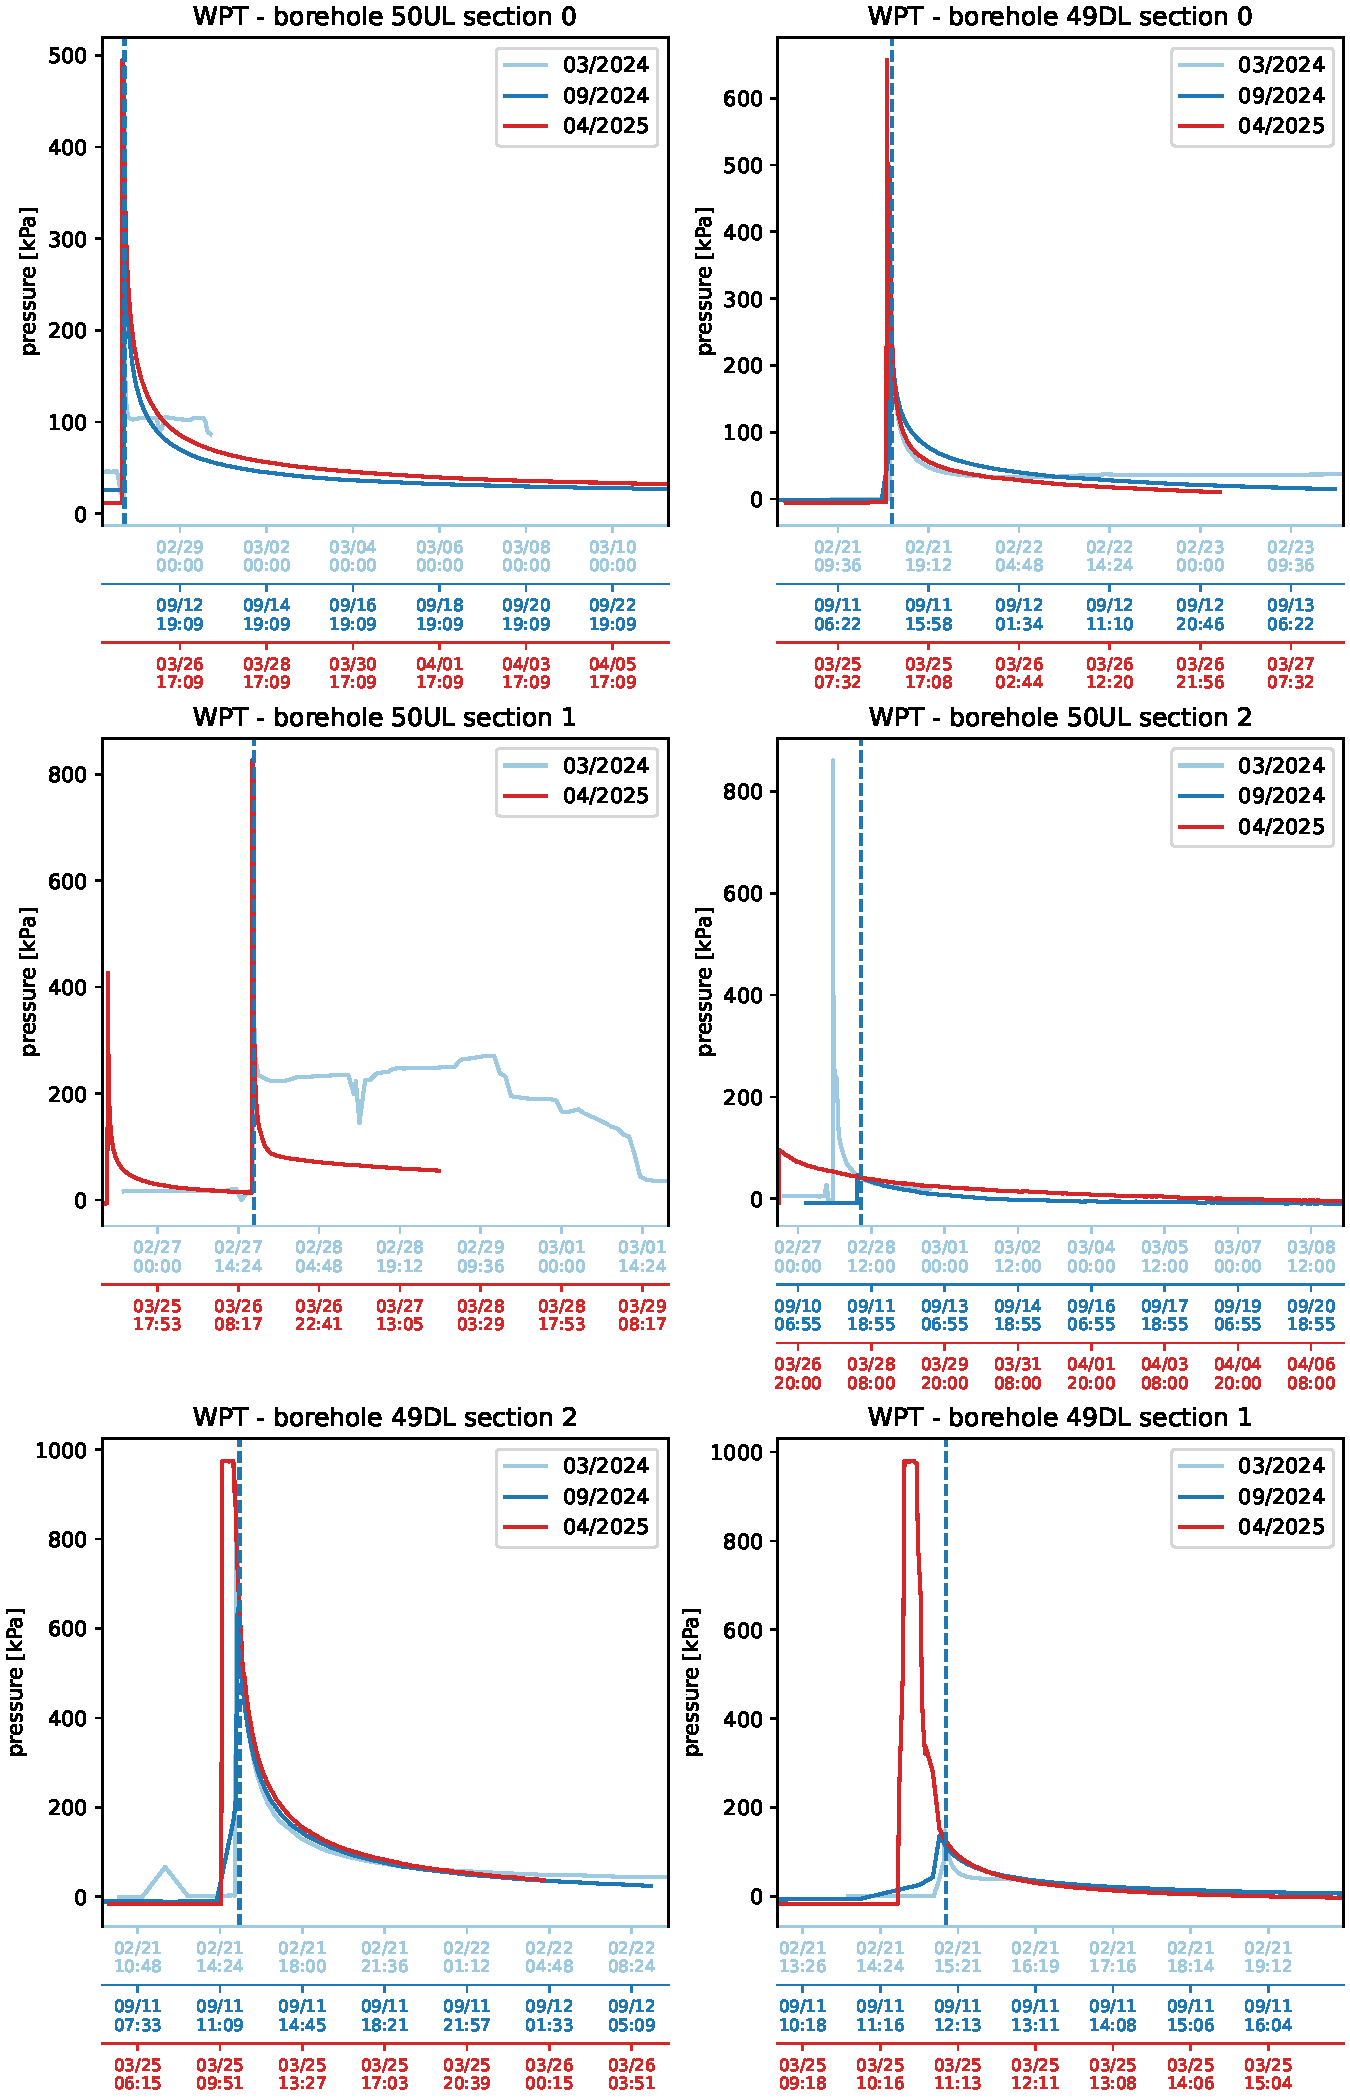
\includegraphics[width=0.9\textwidth]{PP_figs/wpt_grid_04.pdf}
    \end{center}
    \caption{Stitched water pressure test plots 04.}
    \label{fig:wpts_cases_19_24}
\end{figure}
\FloatBarrier
\newpage
\begin{figure}
    \begin{center}
    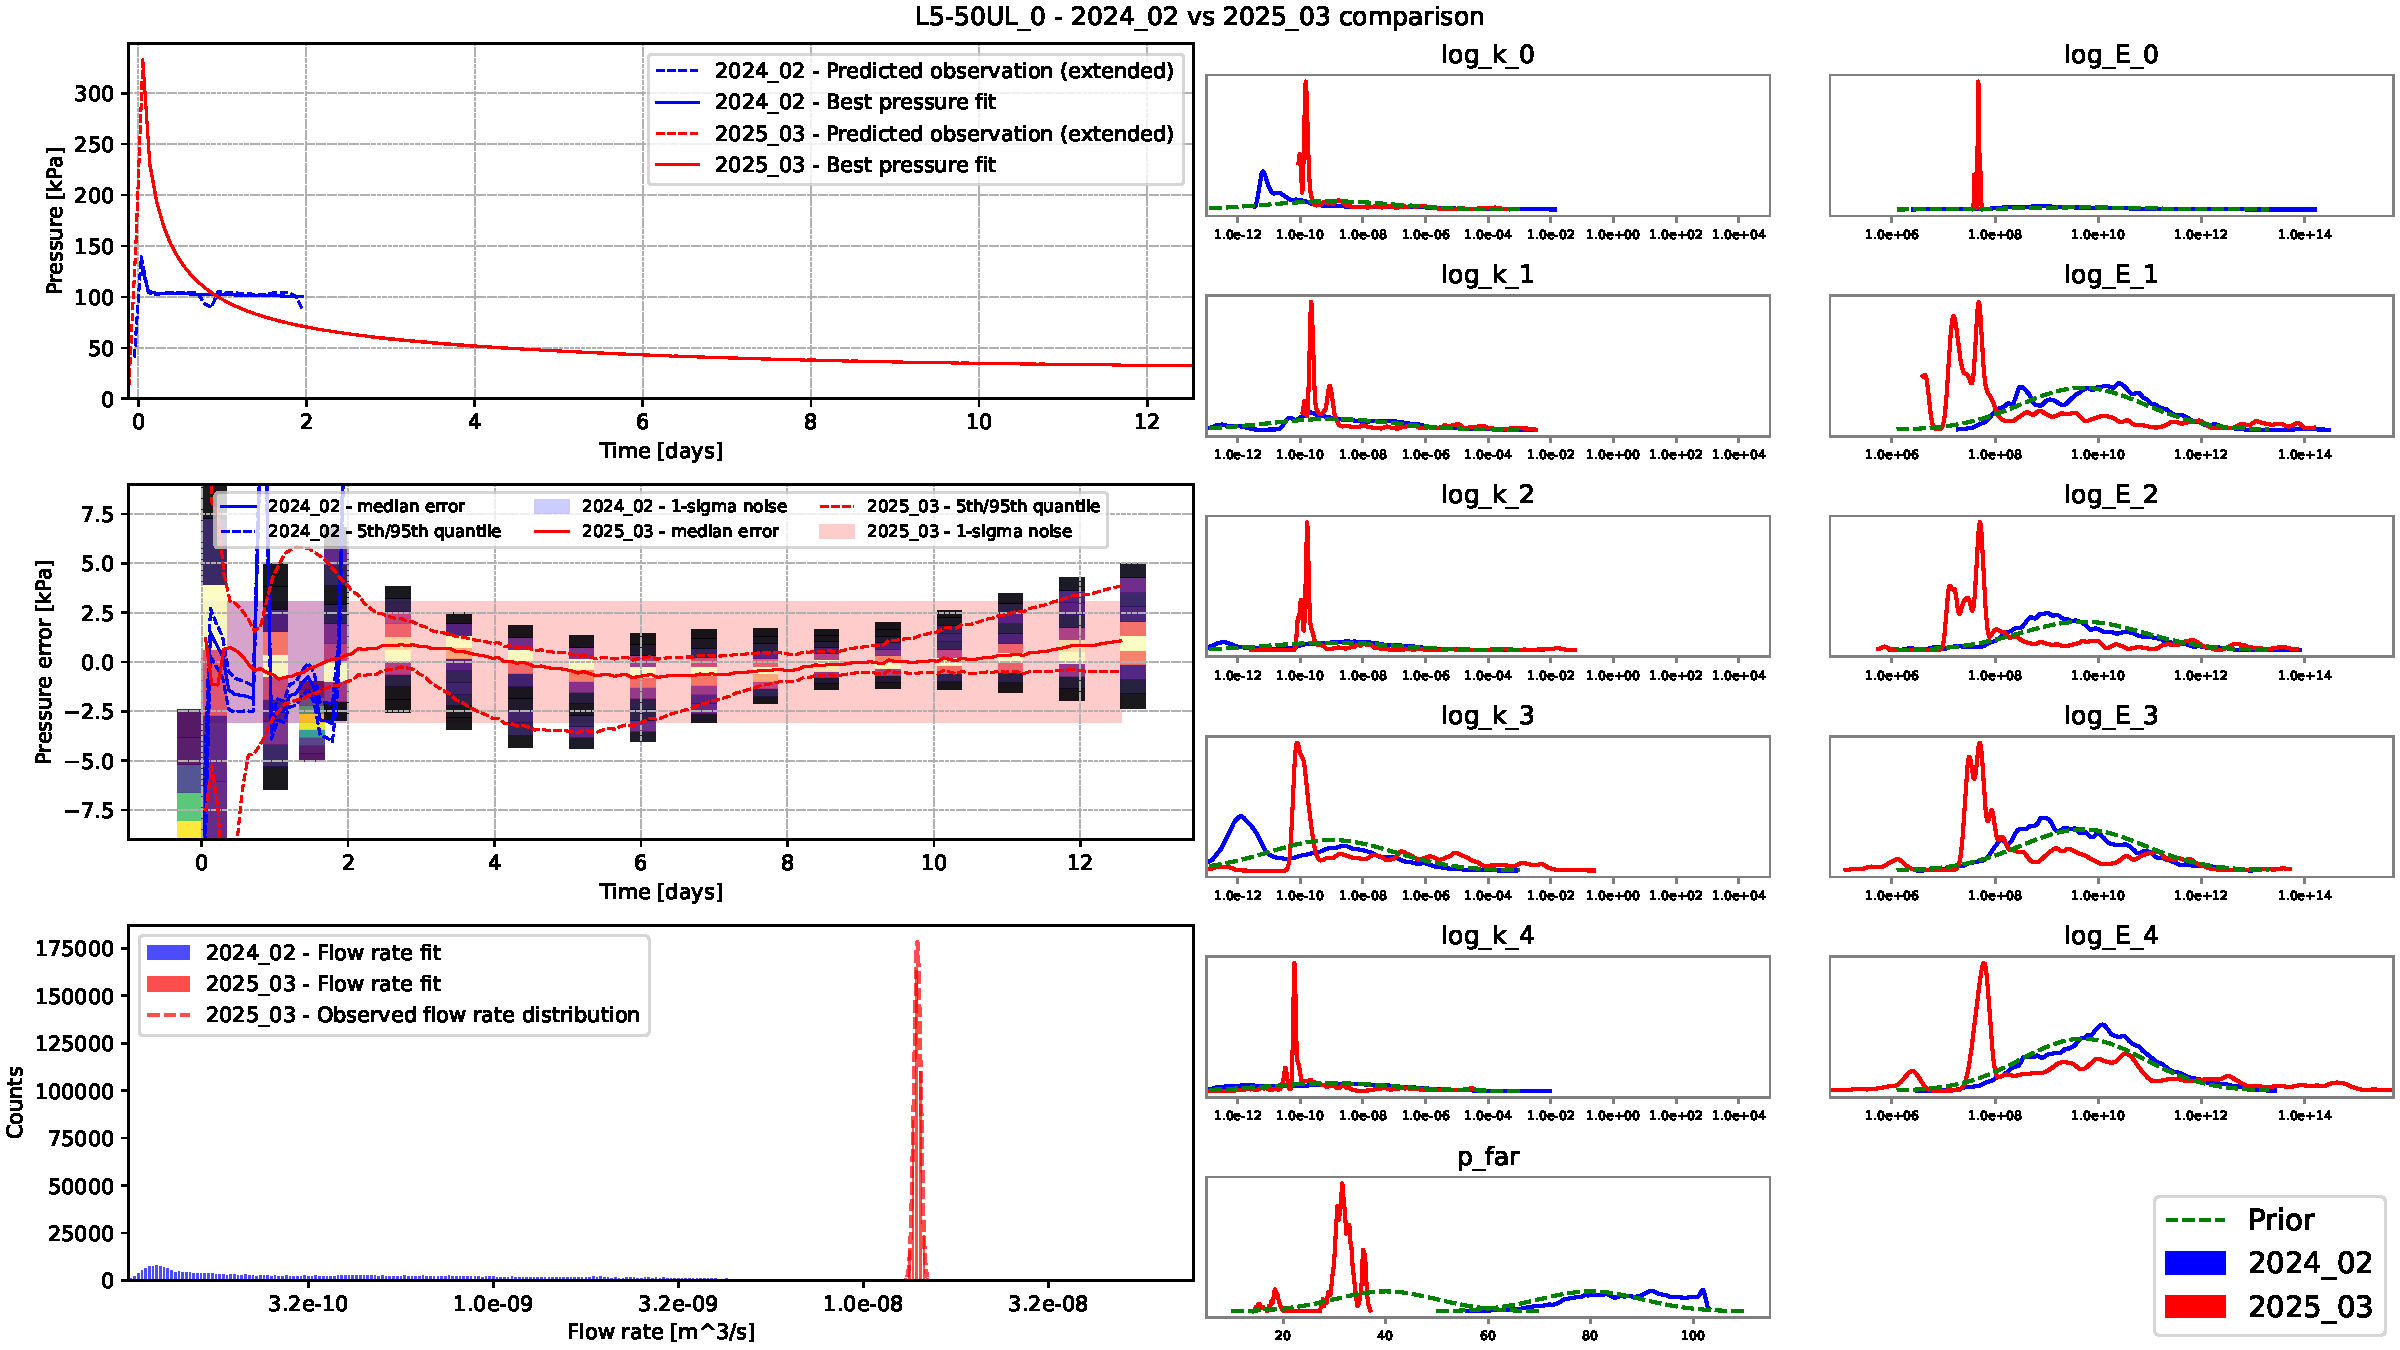
\includegraphics[width=0.75\textwidth]{PP_figs/50UL_0_compareplot.pdf}
    \end{center}
    \caption{Bayesian inversion summary for cell 50UL-0.}
    \label{fig:bayes_50UL_0}
\end{figure}
\begin{figure}
    \begin{center}
    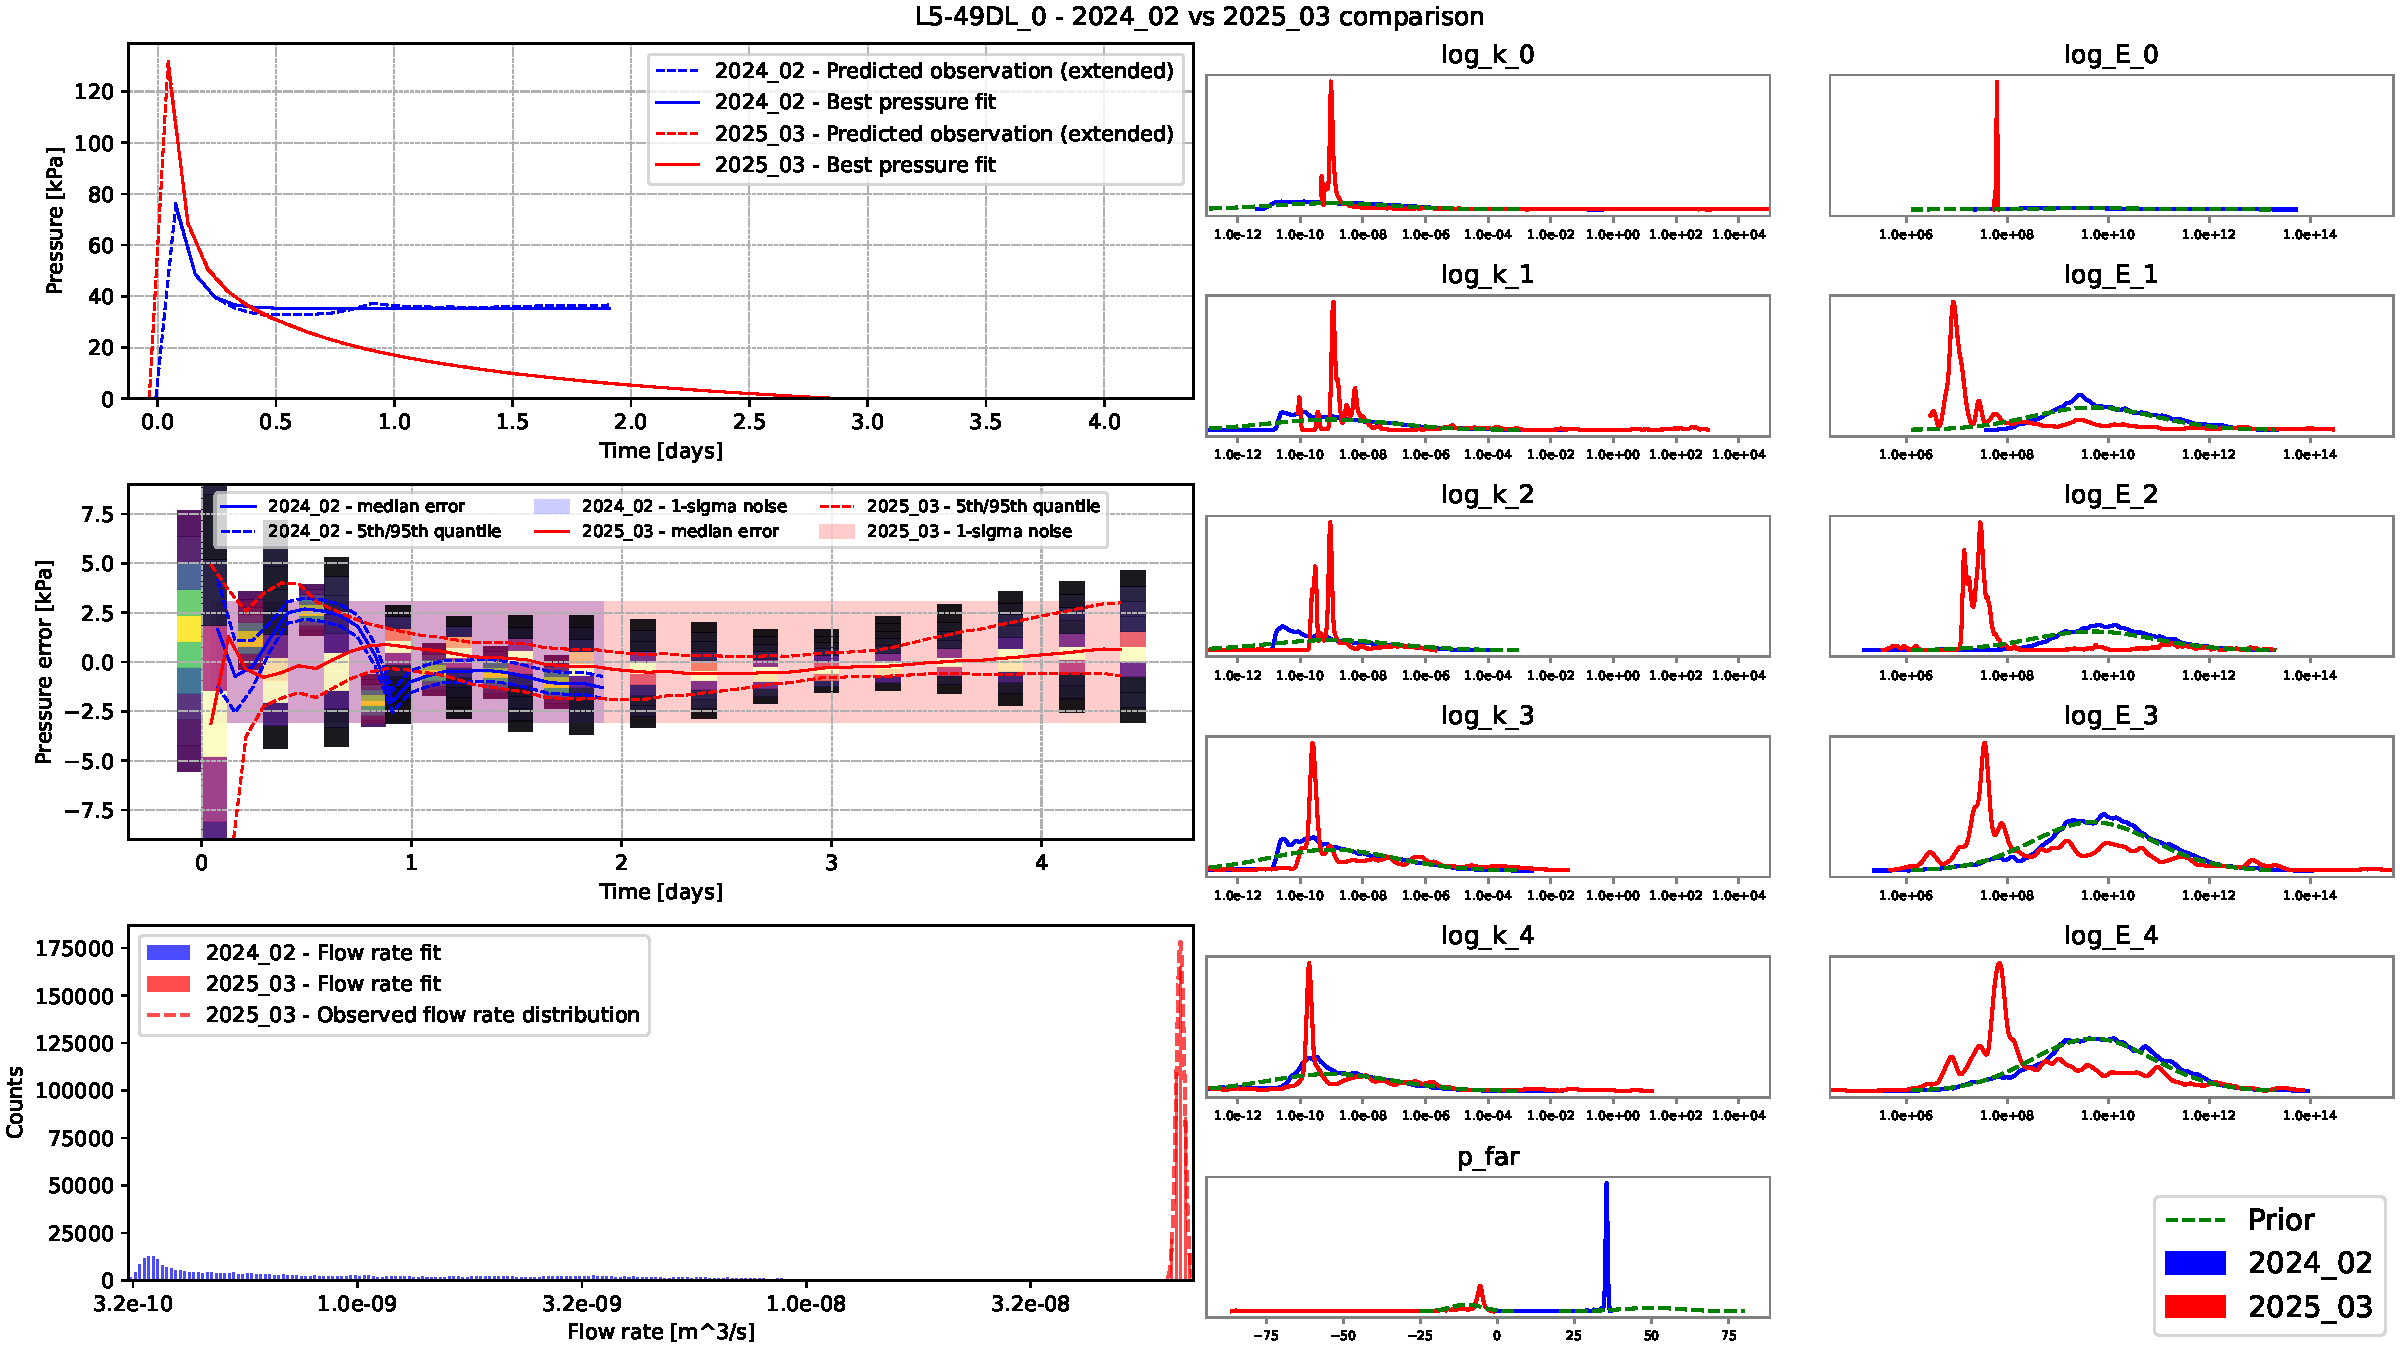
\includegraphics[width=0.75\textwidth]{PP_figs/49DL_0_compareplot.pdf}
    \end{center}
    \caption{Bayesian inversion summary for cell 49DL-0.}
    \label{fig:bayes_49DL_0}
\end{figure}
\begin{figure}
    \begin{center}
    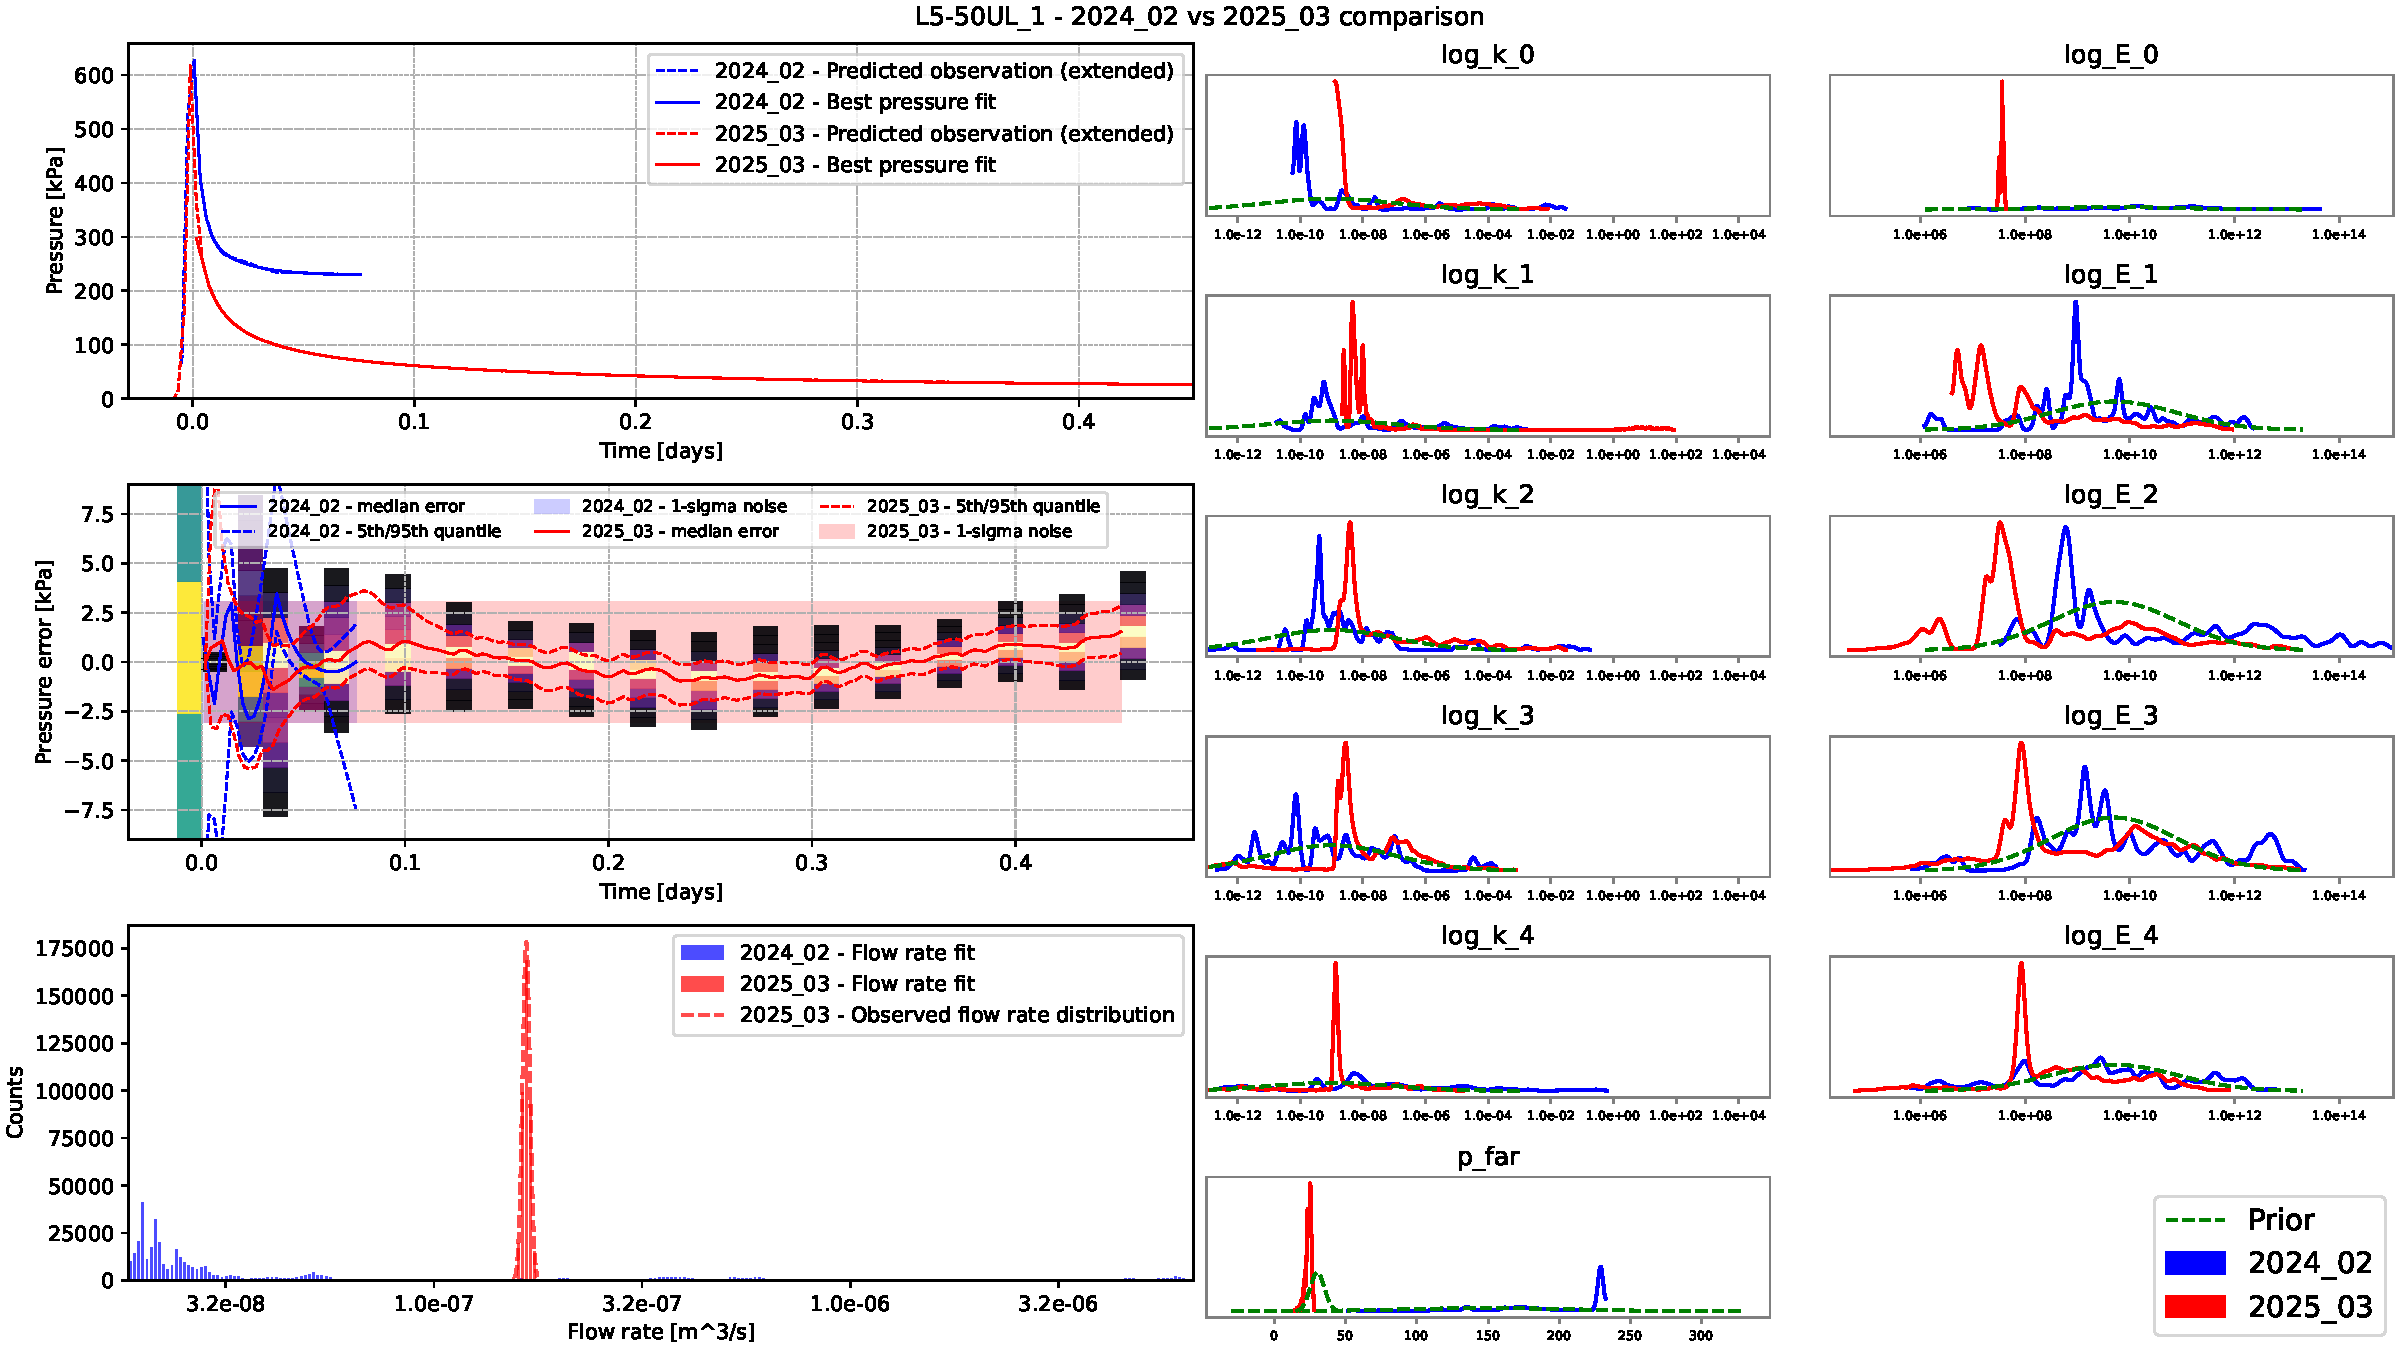
\includegraphics[width=0.75\textwidth]{PP_figs/50UL_1_compareplot.pdf}
    \end{center}
    \caption{Bayesian inversion summary for cell 50UL-1.}
    \label{fig:bayes_50UL_1}
\end{figure}
\FloatBarrier
\newpage
\begin{figure}
    \begin{center}
    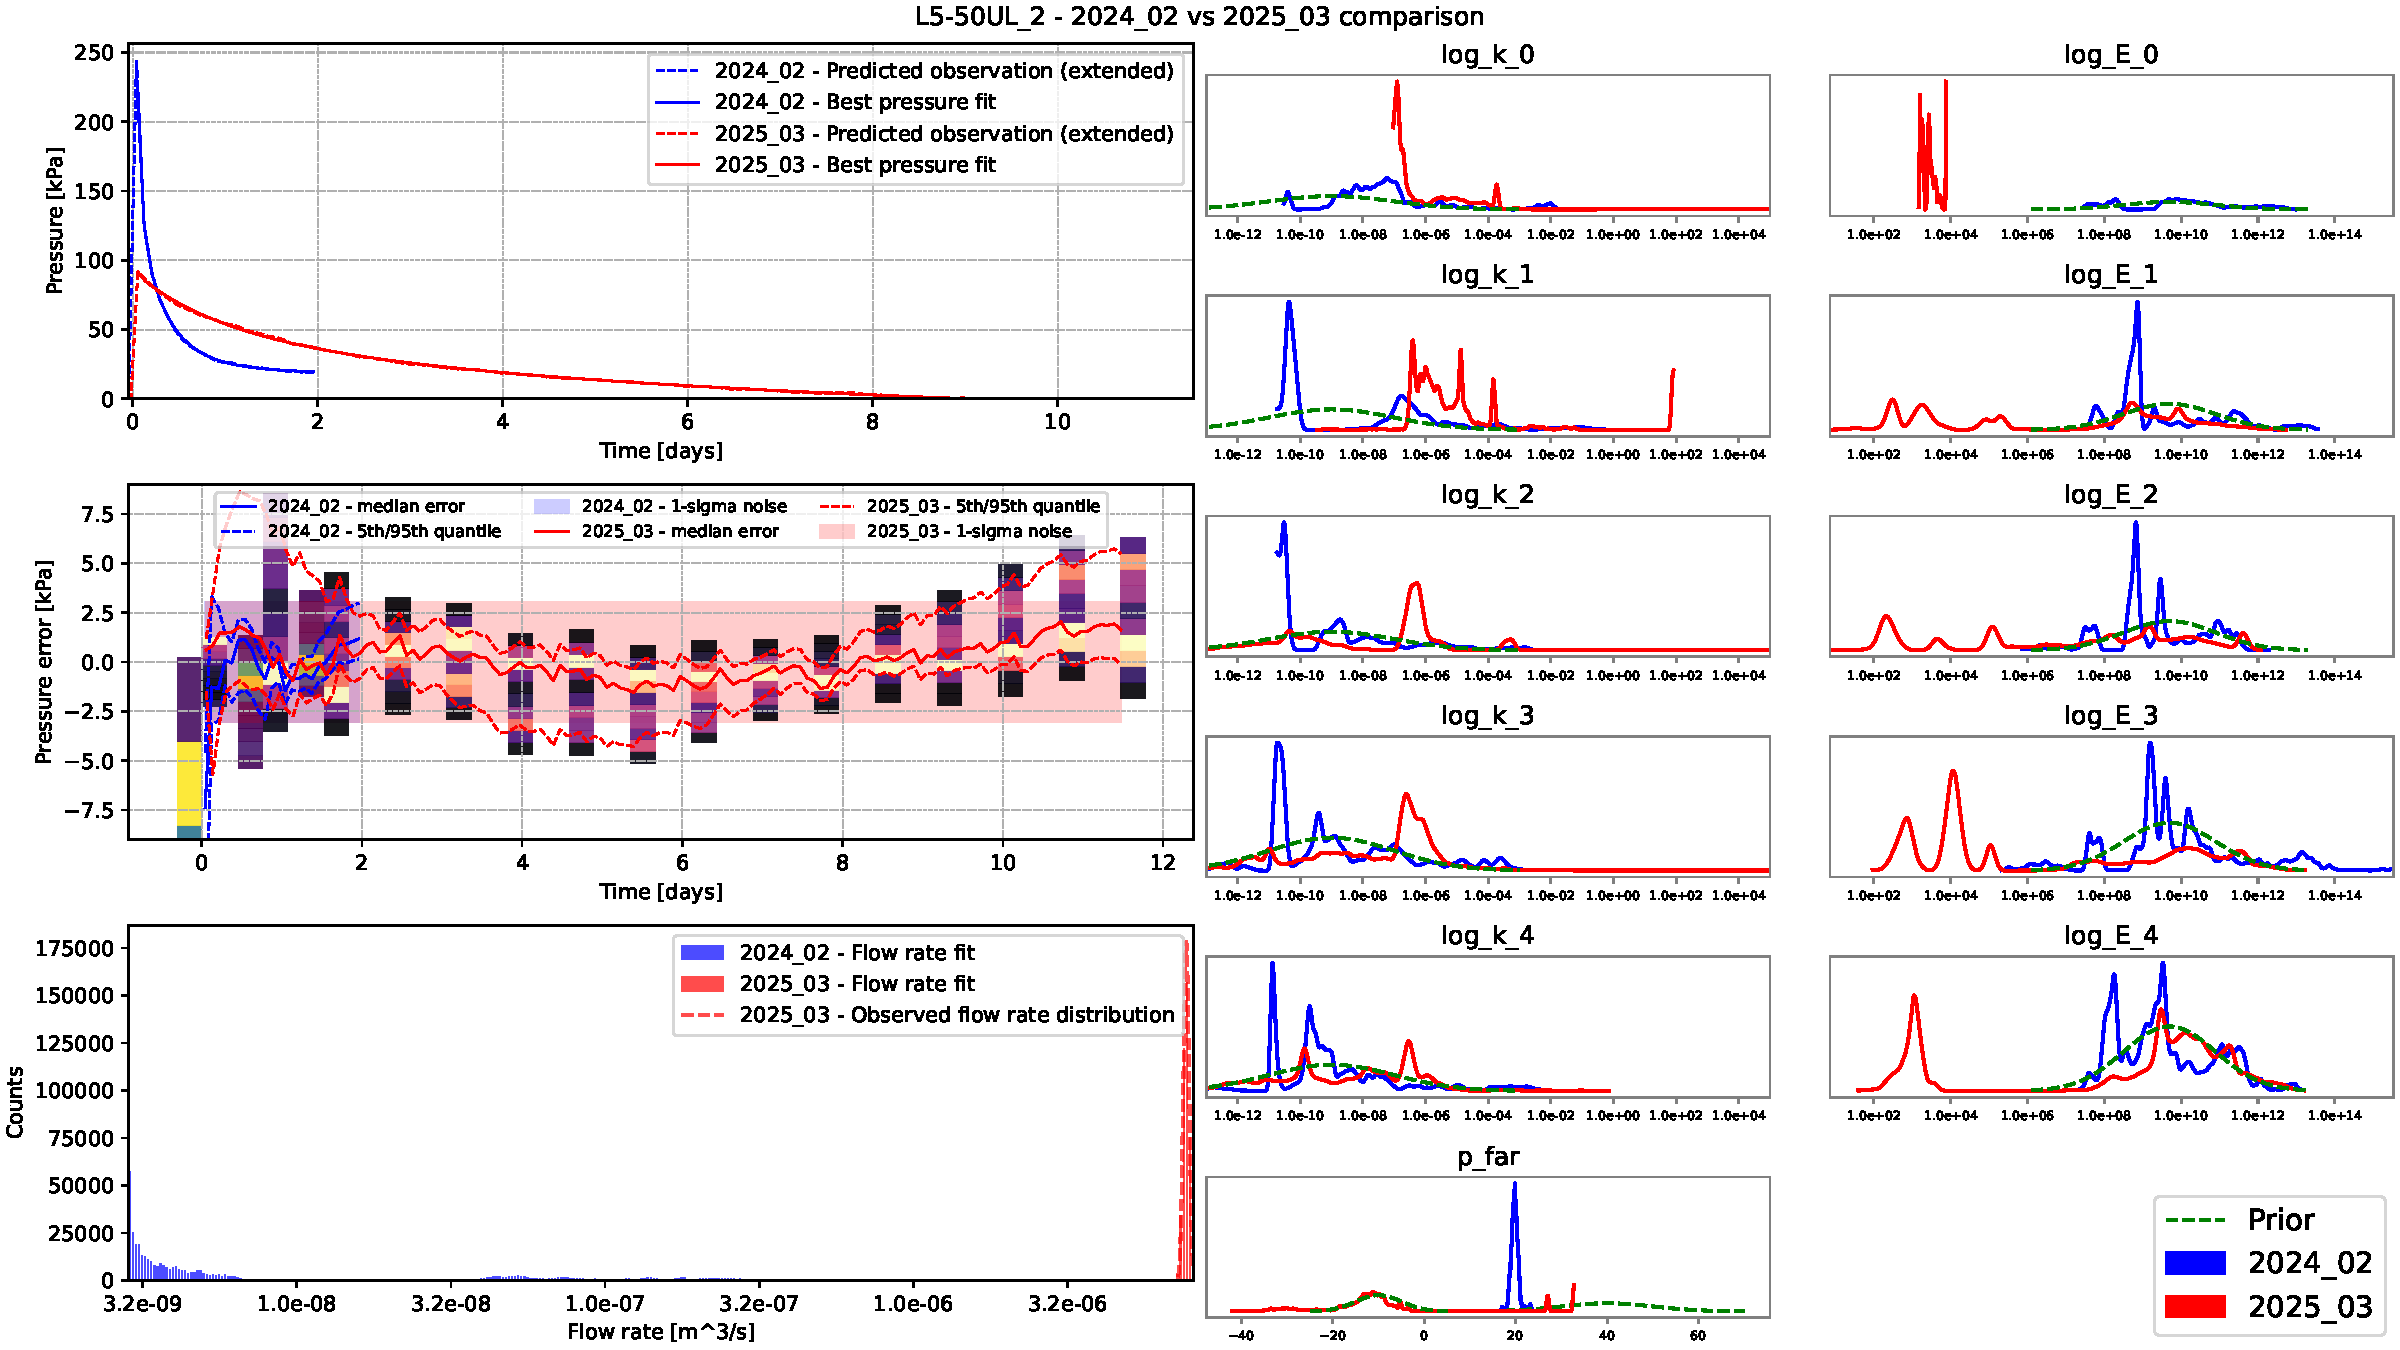
\includegraphics[width=0.75\textwidth]{PP_figs/50UL_2_compareplot.pdf}
    \end{center}
    \caption{Bayesian inversion summary for cell 50UL-2.}
    \label{fig:bayes_50UL_2}
\end{figure}
\begin{figure}
    \begin{center}
    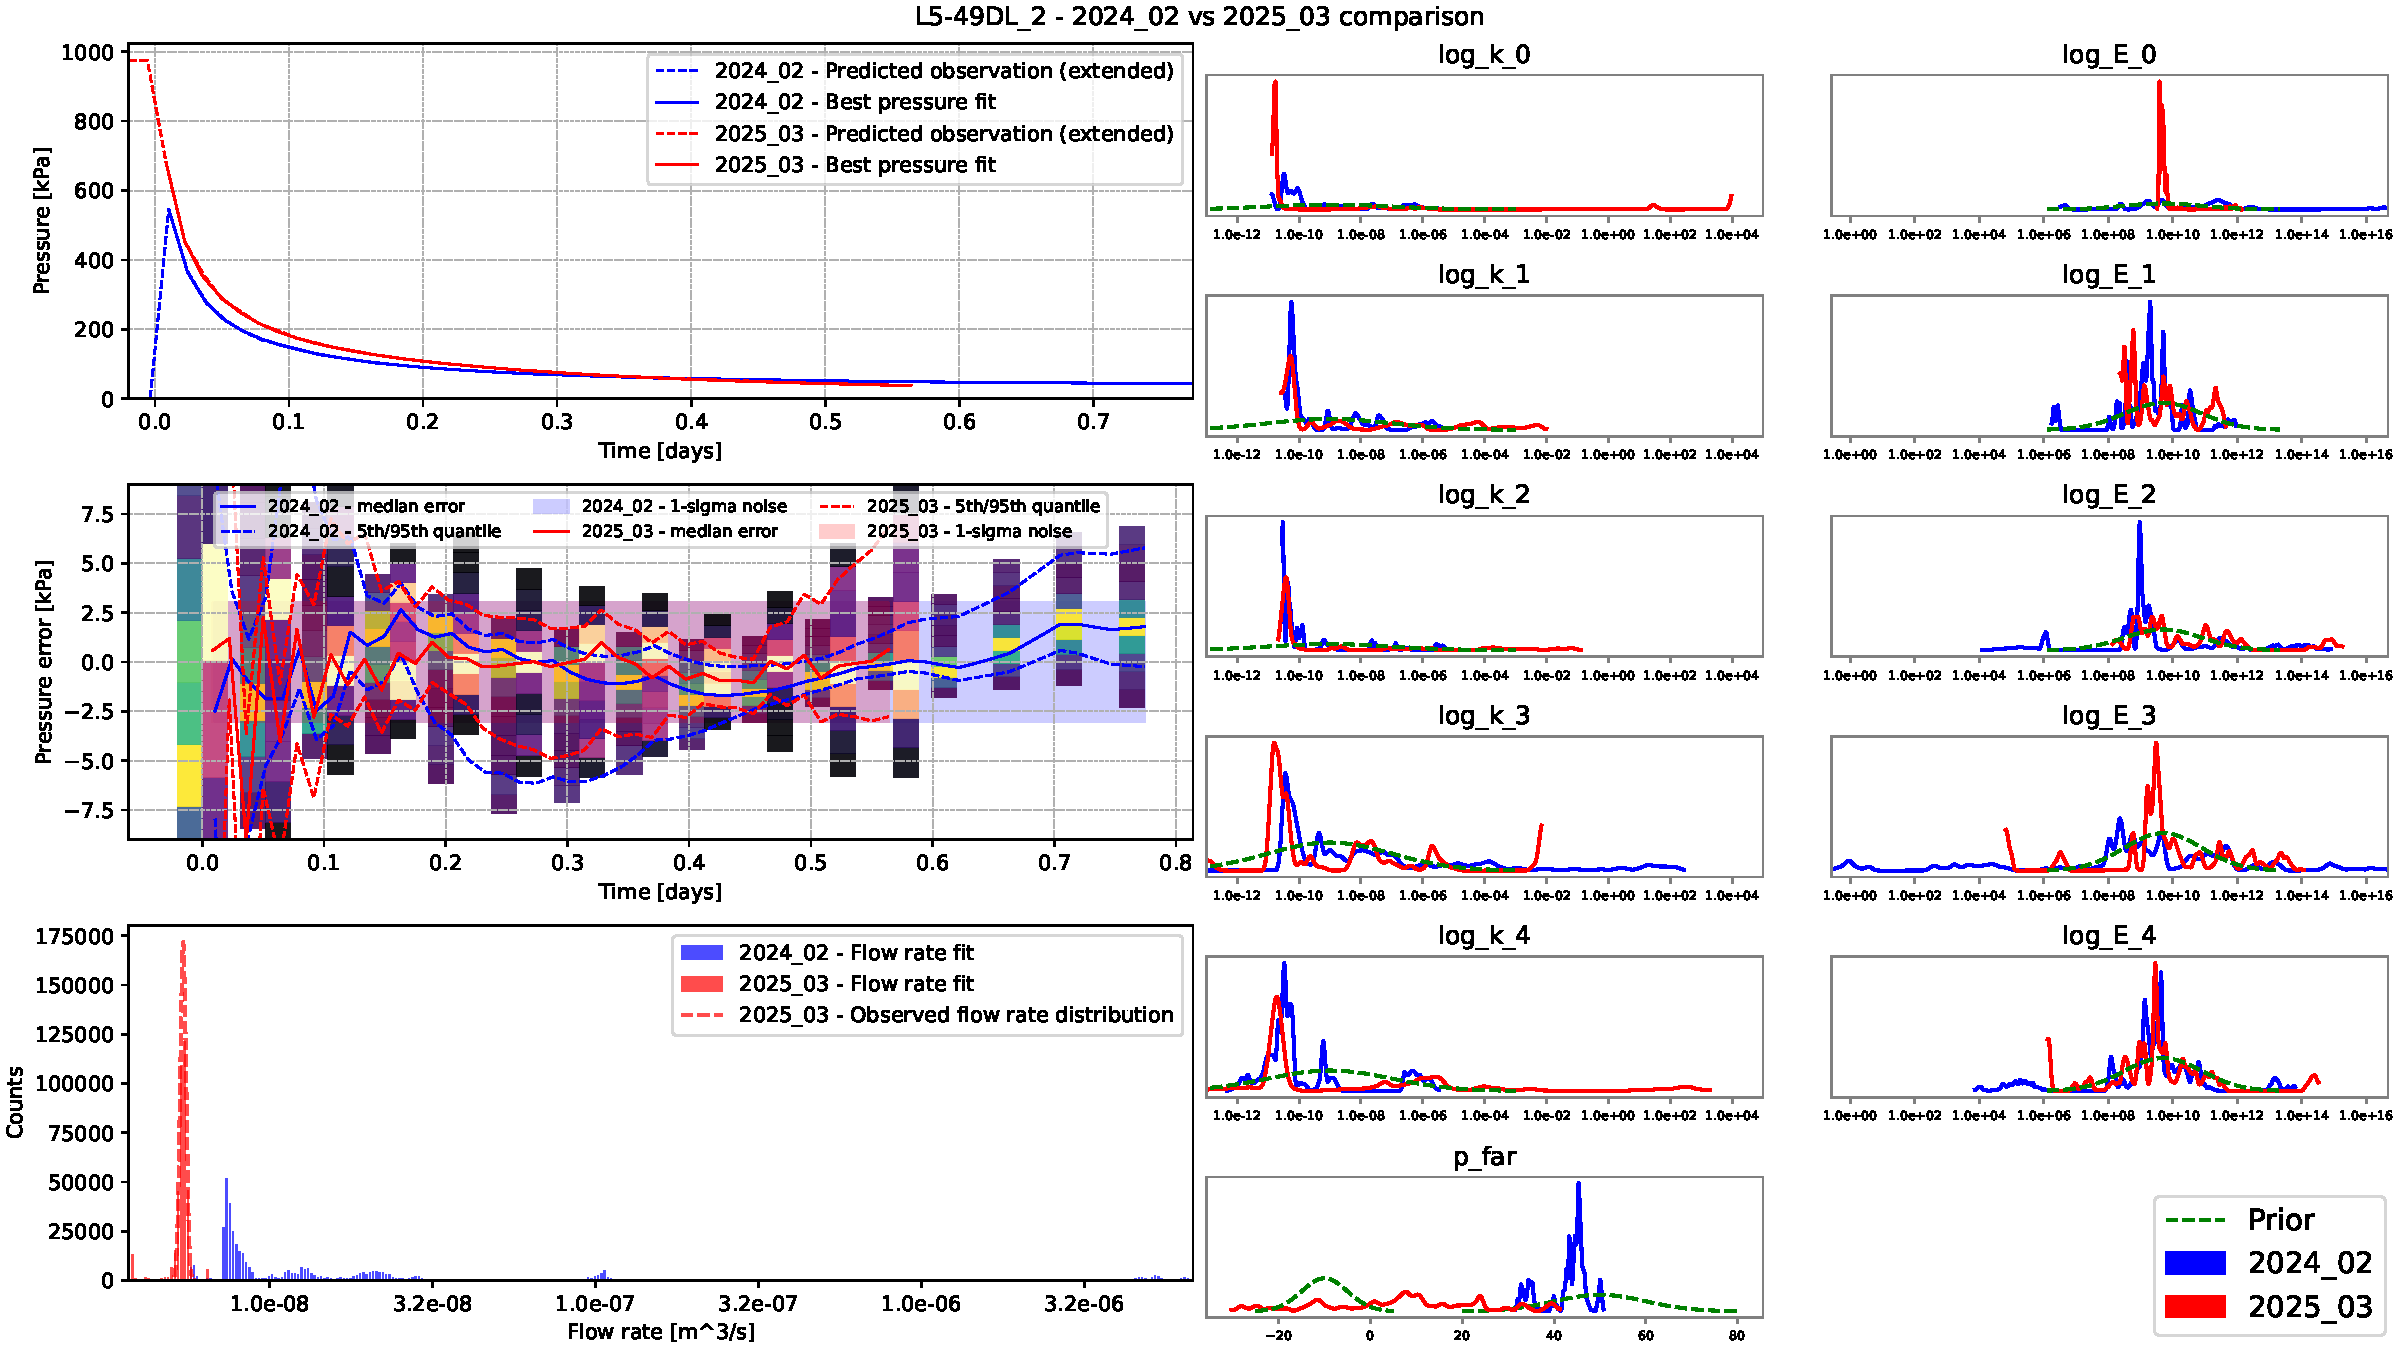
\includegraphics[width=0.75\textwidth]{PP_figs/49DL_2_compareplot.pdf}
    \end{center}
    \caption{Bayesian inversion summary for cell 49DL-2.}
    \label{fig:bayes_49DL_2}
\end{figure}
\begin{figure}
    \begin{center}
    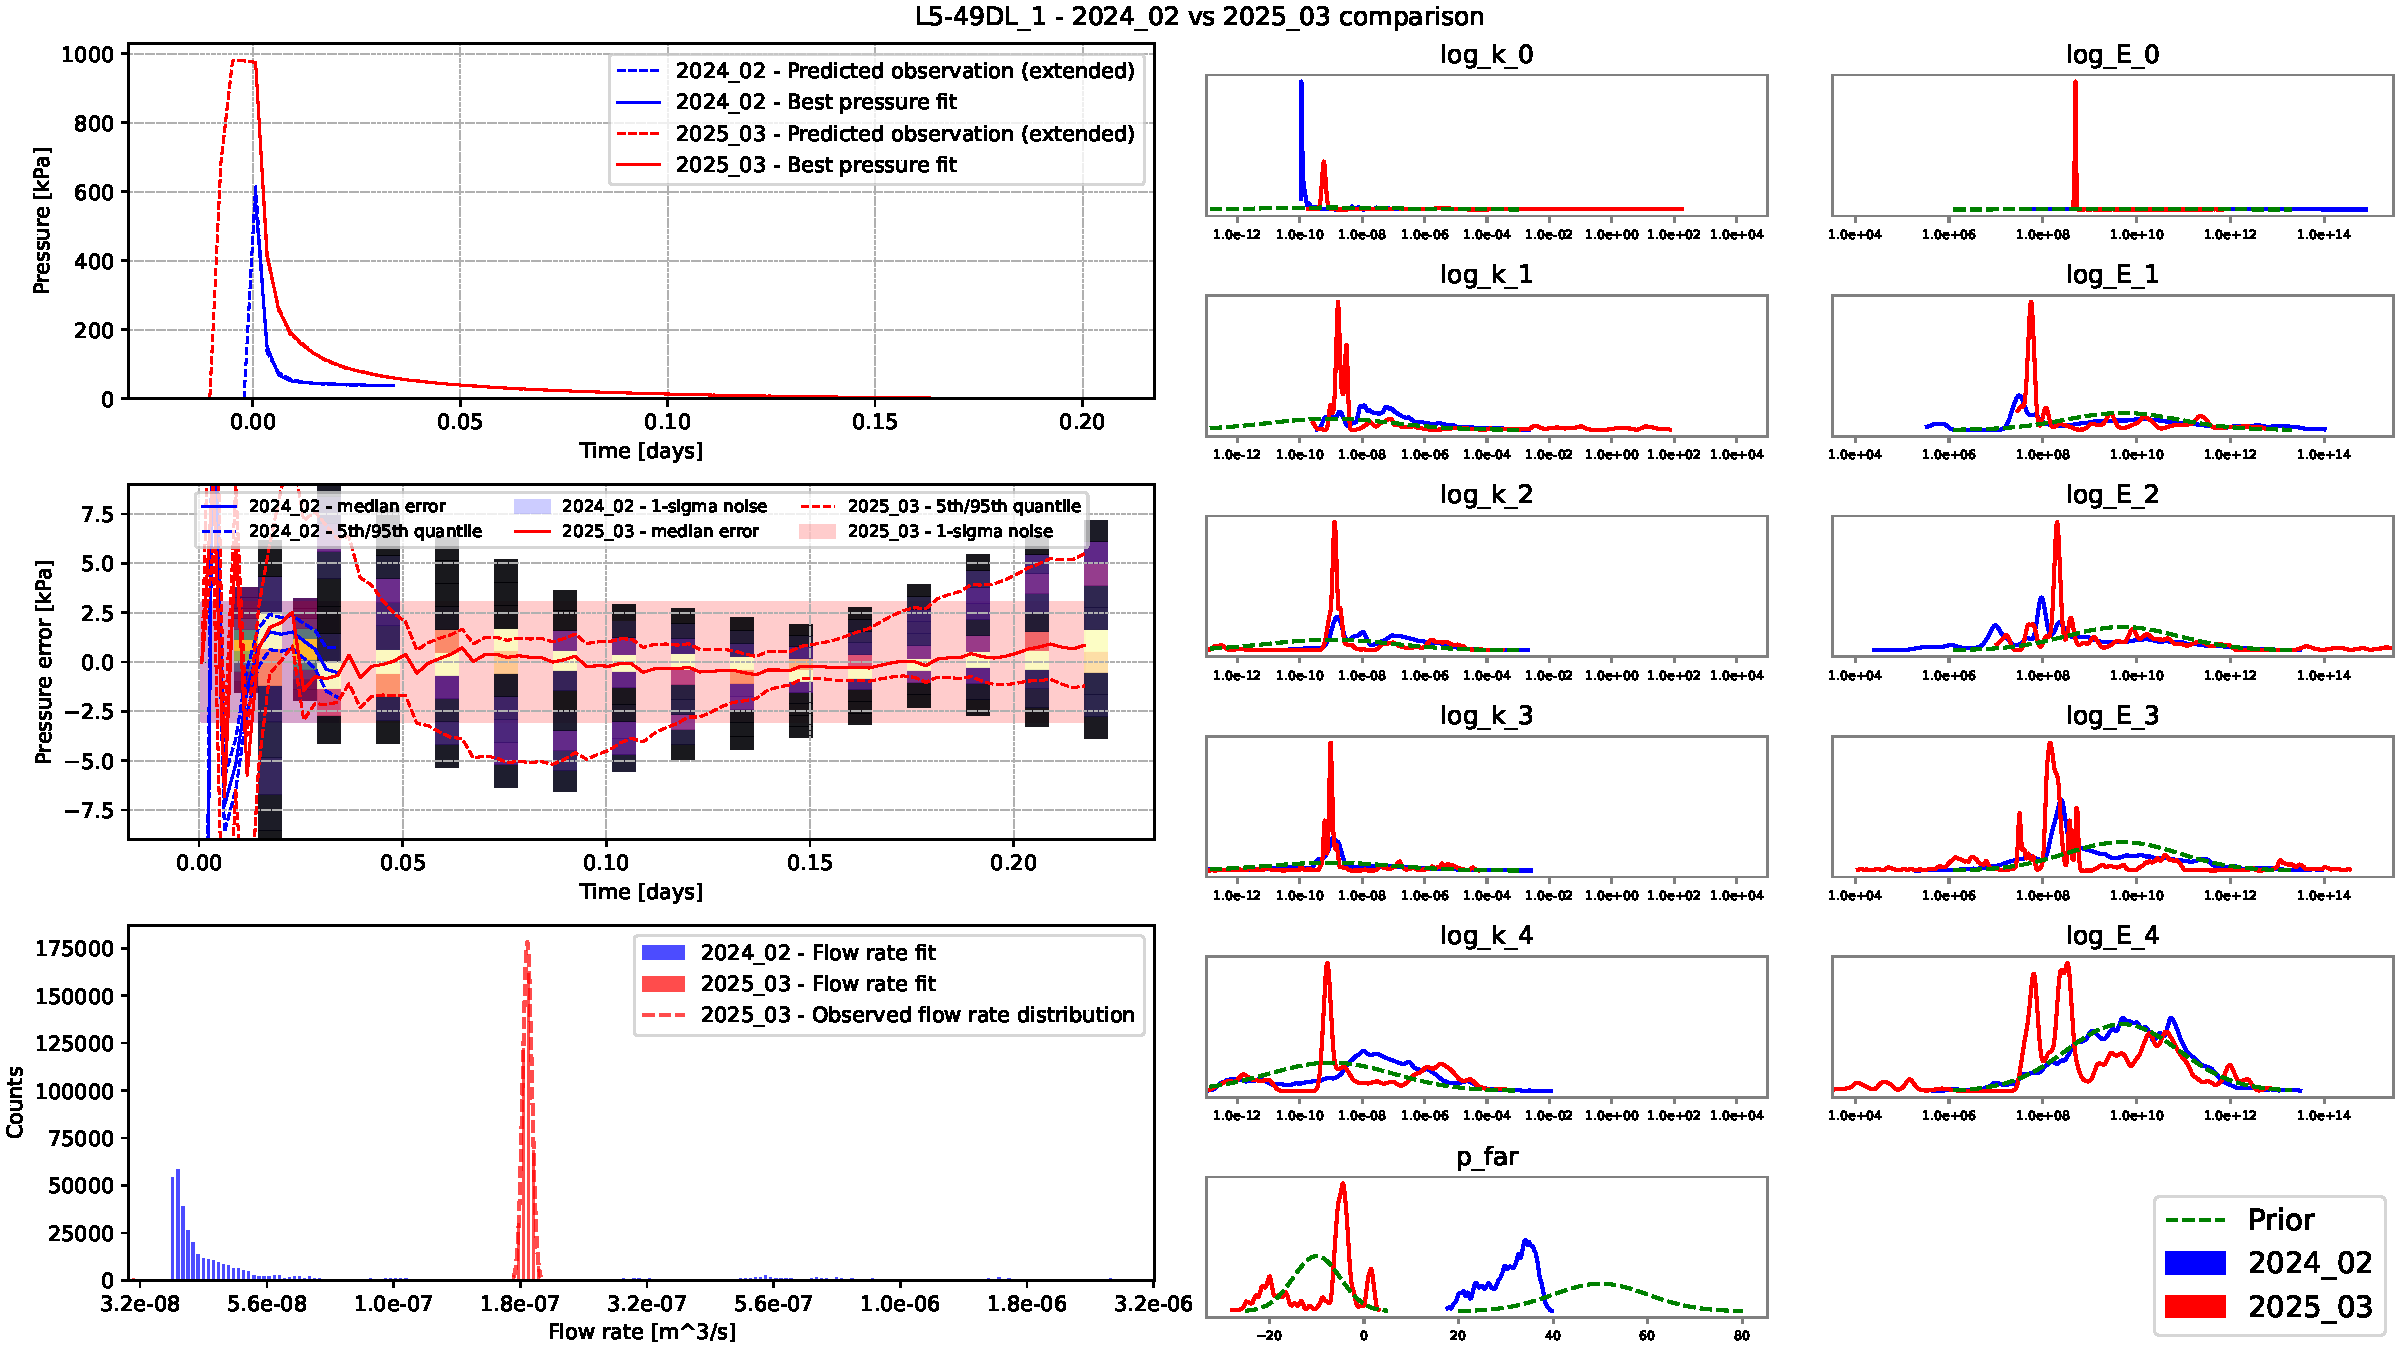
\includegraphics[width=0.75\textwidth]{PP_figs/49DL_1_compareplot.pdf}
    \end{center}
    \caption{Bayesian inversion summary for cell 49DL-1.}
    \label{fig:bayes_49DL_1}
\end{figure}
\FloatBarrier
\newpage

\subsection{Summary}
All installed pressure sensors exhibit an excellent signal-to-noise ratio. A response
to excavation is observable on all sensors, and more than half show a very pronounced
response. Most signal features are temporally associated with the WPTs, drilling of
blast holes, and the blast events themselves; however, a few short-term anomalies
that are not synchronized with these activities are also present and remain
unexplained.

Overall, the excavation-induced pressure changes are much smaller than predicted by
the homogeneous hydro-mechanical model (see Section~\ref{3D_excavation_model}) when using hydraulic
and elastic parameters consistent with previous measurements (Chapter~\ref{chapter:review}).
Several systematic deviations from the model are observed: pressure peaks and drops
occur at locations different from those predicted for a homogeneous medium, and some
blast-related responses indicate highly conductive hydraulic connections. The contrast
between the southern and northern chambers is also notable: the northern sensors show
similar patterns but with smaller amplitudes, consistent with overall higher
conductivity and/or reduced stiffness in the northern rock mass.

A recurring pattern observed in several initial WPTs is a rapid pressure decrease
followed by a sustained increase toward a higher apparent equilibrium pressure.
This behavior cannot be explained by rock heterogeneity alone. The initial WPTs were
likely affected by prior drainage along the drilled boreholes, which implies the
presence of highly conductive fractures capable of producing substantial drainage
over a period of roughly 14~days. Additional indications of fractures include
correlations between sensor signals after WPTs. The excavation-period records also
point to a key role of fractures, as shown by the missing response to the third south
blast and by pressure peaks and drops occurring at locations different from those
predicted by the homogeneous model. Some of these features may also be influenced by
foliation-related anisotropy in hydraulic conductivity, the Biot tensor, and the
elasticity tensor.

Nearly all sensors exhibit long-term drift or slow evolution of the apparent
equilibrium pressure, which complicates direct comparison of pre- and
post-excavation states. Intentional short depressurization and measurement of the
common atmospheric pressure before repeated WPTs could help to identify and exclude
drift caused by the sensors themselves.

The initial WPTs were substantially affected by the preceding borehole drilling and
by insufficient time for pressure equilibration, both before the WPTs and before the
start of excavation. In addition, the lack of water-flux measurements during the
2024 WPTs significantly increases the ambiguity in distinguishing between the
effects of hydraulic conductivity and stiffness in the inversion.

Based on this experience, we recommend the following procedure for future
experiments:
\begin{enumerate}
\item \textbf{Initial conditioning pressurization:} Pressurize each cell to the
expected equilibrium pressure.
\item \textbf{Pre-test equilibration monitoring:} Monitor pressure for about
14~days. Use the relaxation curve to extrapolate the equilibrium pressure and, if
needed, adjust the initial pressurization level.
\item \textbf{Stepwise WPT with flux measurements:} Perform the WPT as a sequence of
pressure steps in geometric progression. Increase the pump flux until the next
pressure step is reached, then maintain constant pump flux (assuming a piston pump) for
15--60~minutes while recording pressure. Proceed earlier if the next pressure level
is reached. End the WPT at a prescribed peak pressure level of at most 1~MPa, adapted
to the effective pump capacity and the hydraulic conductivity of the cell.
\item \textbf{Long-term pressure relaxation:} Leave the cell pressurized at the
peak pressure and monitor pressure equilibration, ideally for about one month, to
improve parameter identifiability.
\item \textbf{Controlled return toward equilibrium:} Use the observed trend to
predict the new equilibrium pressure and manually reduce pressure toward this level.
\item \textbf{Post-test equilibration before excavation:} Allow a further
equilibration period of at least 14~days. Excavation can then begin with sensors in a
well-defined initial state.
\end{enumerate}


